\documentclass[]{book}
\usepackage{lmodern}
\usepackage{amssymb,amsmath}
\usepackage{ifxetex,ifluatex}
\usepackage{fixltx2e} % provides \textsubscript
\ifnum 0\ifxetex 1\fi\ifluatex 1\fi=0 % if pdftex
  \usepackage[T1]{fontenc}
  \usepackage[utf8]{inputenc}
\else % if luatex or xelatex
  \ifxetex
    \usepackage{mathspec}
  \else
    \usepackage{fontspec}
  \fi
  \defaultfontfeatures{Ligatures=TeX,Scale=MatchLowercase}
\fi
% use upquote if available, for straight quotes in verbatim environments
\IfFileExists{upquote.sty}{\usepackage{upquote}}{}
% use microtype if available
\IfFileExists{microtype.sty}{%
\usepackage{microtype}
\UseMicrotypeSet[protrusion]{basicmath} % disable protrusion for tt fonts
}{}
\usepackage[margin=1in]{geometry}
\usepackage{hyperref}
\hypersetup{unicode=true,
            pdftitle={CAS Exam 9 Study Notes},
            pdfauthor={Cliff Lau},
            pdfborder={0 0 0},
            breaklinks=true}
\urlstyle{same}  % don't use monospace font for urls
\usepackage{color}
\usepackage{fancyvrb}
\newcommand{\VerbBar}{|}
\newcommand{\VERB}{\Verb[commandchars=\\\{\}]}
\DefineVerbatimEnvironment{Highlighting}{Verbatim}{commandchars=\\\{\}}
% Add ',fontsize=\small' for more characters per line
\usepackage{framed}
\definecolor{shadecolor}{RGB}{248,248,248}
\newenvironment{Shaded}{\begin{snugshade}}{\end{snugshade}}
\newcommand{\KeywordTok}[1]{\textcolor[rgb]{0.13,0.29,0.53}{\textbf{{#1}}}}
\newcommand{\DataTypeTok}[1]{\textcolor[rgb]{0.13,0.29,0.53}{{#1}}}
\newcommand{\DecValTok}[1]{\textcolor[rgb]{0.00,0.00,0.81}{{#1}}}
\newcommand{\BaseNTok}[1]{\textcolor[rgb]{0.00,0.00,0.81}{{#1}}}
\newcommand{\FloatTok}[1]{\textcolor[rgb]{0.00,0.00,0.81}{{#1}}}
\newcommand{\ConstantTok}[1]{\textcolor[rgb]{0.00,0.00,0.00}{{#1}}}
\newcommand{\CharTok}[1]{\textcolor[rgb]{0.31,0.60,0.02}{{#1}}}
\newcommand{\SpecialCharTok}[1]{\textcolor[rgb]{0.00,0.00,0.00}{{#1}}}
\newcommand{\StringTok}[1]{\textcolor[rgb]{0.31,0.60,0.02}{{#1}}}
\newcommand{\VerbatimStringTok}[1]{\textcolor[rgb]{0.31,0.60,0.02}{{#1}}}
\newcommand{\SpecialStringTok}[1]{\textcolor[rgb]{0.31,0.60,0.02}{{#1}}}
\newcommand{\ImportTok}[1]{{#1}}
\newcommand{\CommentTok}[1]{\textcolor[rgb]{0.56,0.35,0.01}{\textit{{#1}}}}
\newcommand{\DocumentationTok}[1]{\textcolor[rgb]{0.56,0.35,0.01}{\textbf{\textit{{#1}}}}}
\newcommand{\AnnotationTok}[1]{\textcolor[rgb]{0.56,0.35,0.01}{\textbf{\textit{{#1}}}}}
\newcommand{\CommentVarTok}[1]{\textcolor[rgb]{0.56,0.35,0.01}{\textbf{\textit{{#1}}}}}
\newcommand{\OtherTok}[1]{\textcolor[rgb]{0.56,0.35,0.01}{{#1}}}
\newcommand{\FunctionTok}[1]{\textcolor[rgb]{0.00,0.00,0.00}{{#1}}}
\newcommand{\VariableTok}[1]{\textcolor[rgb]{0.00,0.00,0.00}{{#1}}}
\newcommand{\ControlFlowTok}[1]{\textcolor[rgb]{0.13,0.29,0.53}{\textbf{{#1}}}}
\newcommand{\OperatorTok}[1]{\textcolor[rgb]{0.81,0.36,0.00}{\textbf{{#1}}}}
\newcommand{\BuiltInTok}[1]{{#1}}
\newcommand{\ExtensionTok}[1]{{#1}}
\newcommand{\PreprocessorTok}[1]{\textcolor[rgb]{0.56,0.35,0.01}{\textit{{#1}}}}
\newcommand{\AttributeTok}[1]{\textcolor[rgb]{0.77,0.63,0.00}{{#1}}}
\newcommand{\RegionMarkerTok}[1]{{#1}}
\newcommand{\InformationTok}[1]{\textcolor[rgb]{0.56,0.35,0.01}{\textbf{\textit{{#1}}}}}
\newcommand{\WarningTok}[1]{\textcolor[rgb]{0.56,0.35,0.01}{\textbf{\textit{{#1}}}}}
\newcommand{\AlertTok}[1]{\textcolor[rgb]{0.94,0.16,0.16}{{#1}}}
\newcommand{\ErrorTok}[1]{\textcolor[rgb]{0.64,0.00,0.00}{\textbf{{#1}}}}
\newcommand{\NormalTok}[1]{{#1}}
\usepackage{longtable,booktabs}
\usepackage{graphicx,grffile}
\makeatletter
\def\maxwidth{\ifdim\Gin@nat@width>\linewidth\linewidth\else\Gin@nat@width\fi}
\def\maxheight{\ifdim\Gin@nat@height>\textheight\textheight\else\Gin@nat@height\fi}
\makeatother
% Scale images if necessary, so that they will not overflow the page
% margins by default, and it is still possible to overwrite the defaults
% using explicit options in \includegraphics[width, height, ...]{}
\setkeys{Gin}{width=\maxwidth,height=\maxheight,keepaspectratio}
\IfFileExists{parskip.sty}{%
\usepackage{parskip}
}{% else
\setlength{\parindent}{0pt}
\setlength{\parskip}{6pt plus 2pt minus 1pt}
}
\setlength{\emergencystretch}{3em}  % prevent overfull lines
\providecommand{\tightlist}{%
  \setlength{\itemsep}{0pt}\setlength{\parskip}{0pt}}
\setcounter{secnumdepth}{5}
% Redefines (sub)paragraphs to behave more like sections
\ifx\paragraph\undefined\else
\let\oldparagraph\paragraph
\renewcommand{\paragraph}[1]{\oldparagraph{#1}\mbox{}}
\fi
\ifx\subparagraph\undefined\else
\let\oldsubparagraph\subparagraph
\renewcommand{\subparagraph}[1]{\oldsubparagraph{#1}\mbox{}}
\fi

%%% Use protect on footnotes to avoid problems with footnotes in titles
\let\rmarkdownfootnote\footnote%
\def\footnote{\protect\rmarkdownfootnote}

%%% Change title format to be more compact
\usepackage{titling}

% Create subtitle command for use in maketitle
\newcommand{\subtitle}[1]{
  \posttitle{
    \begin{center}\large#1\end{center}
    }
}

\setlength{\droptitle}{-2em}
  \title{CAS Exam 9 Study Notes}
  \pretitle{\vspace{\droptitle}\centering\huge}
  \posttitle{\par}
  \author{Cliff Lau}
  \preauthor{\centering\large\emph}
  \postauthor{\par}
  \predate{\centering\large\emph}
  \postdate{\par}
  \date{2017-01-19}


\usepackage{amsthm}
\newtheorem{theorem}{Theorem}[chapter]
\newtheorem{lemma}{Lemma}[chapter]
\theoremstyle{definition}
\newtheorem{definition}{Definition}[chapter]
\newtheorem{corollary}{Corollary}[chapter]
\newtheorem{proposition}{Proposition}[chapter]
\theoremstyle{definition}
\newtheorem{example}{Example}[chapter]
\theoremstyle{remark}
\newtheorem*{remark}{Remark}
\begin{document}
\maketitle

{
\setcounter{tocdepth}{1}
\tableofcontents
}
\chapter{Prerequisites}\label{prerequisites}

This is a \emph{sample} book written in \textbf{Markdown}. You can use
anything that Pandoc's Markdown supports, e.g., a math equation
\(a^2 + b^2 = c^2\).

For now, you have to install the development versions of
\textbf{bookdown} from Github:

\begin{Shaded}
\begin{Highlighting}[]
\NormalTok{devtools::}\KeywordTok{install_github}\NormalTok{(}\StringTok{"rstudio/bookdown"}\NormalTok{)}
\end{Highlighting}
\end{Shaded}

Remember each Rmd file contains one and only one chapter, and a chapter
is defined by the first-level heading \texttt{\#}.

To compile this example to PDF, you need to install XeLaTeX.

\chapter{A1 BKM 6: Risk Averison \& Capital Allocation to Risk
Assets}\label{a1-bkm-6-risk-averison-capital-allocation-to-risk-assets}

Z. Bodie, A. Kane, A. Marcus

\section{Cliff's Summary}\label{cliffs-summary}

Need to memorize and know all the equations by heart and what they
represent

Utility: \(U = \operatorname{E}[r] - 0.5A\sigma^2\)

\begin{itemize}
\tightlist
\item
  \(A > 0\): Risk adverse
\end{itemize}

\protect\hyperlink{CE}{CE}:
\(U = \operatorname{E}[r_f] = \operatorname{E}[r] - 0.5A\sigma^2\)

Complete portfolio \(c\):

\begin{itemize}
\item
  \(\operatorname{E}[r_c] = r_f + \dfrac{\sigma_c}{\sigma_p}\left( \operatorname{E}[r_p] - r_f \right) = r_f + \sigma_c \cdot (\text{Sharpe Ratio})\)
\item
  \(\sigma_c = y \sigma_p\)
\end{itemize}

\protect\hyperlink{CAL}{Capital allocation line}

\begin{itemize}
\tightlist
\item
  Capital market line is the CAL that uses a passive portfolio as the
  risky portfolio
\end{itemize}

Sharpe Ratio: \(\dfrac{\operatorname{E}[r_p] - r_f}{\sigma_p}\)

Optimal complete portfolio ratio on risky asset:
\(y^* = \dfrac{\operatorname{E}[r_p] - r_f}{A\sigma^2_p}\)

\protect\hyperlink{graphically}{Graphically} derive optimal risk
portfolio with indifference curves

\begin{itemize}
\tightlist
\item
  Curves that contain different portfolios that the investor is
  indifferent about, given the same \(U\) and \(A\)
\end{itemize}

\subsection{Types of Exam Questions}\label{types-of-exam-questions}

{Haven't done TIA practice questions}

\textbf{Return and \(\sigma\)}

\begin{itemize}
\tightlist
\item
  \protect\hyperlink{2003-3}{2003, Q3}: return and \(\sigma\) and risk
  premium
\item
  \protect\hyperlink{2003-4}{2003, Q4}: plug and play to formula for
  expected return for complete portfolio
\item
  2004, Q3: plug and play return and \(\sigma\)
\item
  2007, Q1 a: complete ptf return and \(\sigma\)
\item
  2010, Q2 a: back out \(\operatorname{E}[r_c]\) with sharpe ratio and
  \(\sigma_c\)
\item
  2013, Q1 b: returna and \(\sigma\) plug and play
\end{itemize}

\textbf{CAL}

\begin{itemize}
\tightlist
\item
  2006, Q4: Draw CAL and the CAL equation
\item
  2007, Q1 b: Draw CAL and CAL equation
\item
  2010, Q2 b: Draw CAL
\item
  2014, Q1: Draw CAL with borrowing restriction
\end{itemize}

\textbf{Utility}

\begin{itemize}
\tightlist
\item
  2005, Q4 b c: utility function calcuation and CE
\item
  \(\star\) \protect\hyperlink{2009-1}{2009, Q1}: Need to convert the
  standard \(y^*\) formula
\item
  2010, Q3: same as above
\item
  2013, Q1 a: CE
\end{itemize}

\textbf{Portfolio Weights}

\begin{itemize}
\tightlist
\item
  \(\star\) \protect\hyperlink{2011-1}{2011, Q1}: get \(y^*\) and
  describe
\item
  \(\star\) \protect\hyperlink{2012-1}{2012, Q1} a: Getting weights for
  each assets
\item
  2013, Q1 c: \(y^*\) plug and play
\end{itemize}

\textbf{Concepts}

\begin{itemize}
\tightlist
\item
  2005, Q4 a: risk neutral implication
\item
  2012, Q1 b: seperation principle (BKM7)
\item
  2014, Q2: active vs passive investment
\end{itemize}

\begin{longtable}[]{@{}lll@{}}
\toprule
\begin{minipage}[b]{0.30\columnwidth}\raggedright\strut
\strut
\end{minipage} & \begin{minipage}[b]{0.30\columnwidth}\raggedright\strut
Active\strut
\end{minipage} & \begin{minipage}[b]{0.30\columnwidth}\raggedright\strut
Passive\strut
\end{minipage}\tabularnewline
\midrule
\endhead
\begin{minipage}[t]{0.30\columnwidth}\raggedright\strut
Constructing Portfolio\strut
\end{minipage} & \begin{minipage}[t]{0.30\columnwidth}\raggedright\strut
Seeks (+)\(\alpha\), picking investment\strut
\end{minipage} & \begin{minipage}[t]{0.30\columnwidth}\raggedright\strut
Replicate diversified portfolio\strut
\end{minipage}\tabularnewline
\begin{minipage}[t]{0.30\columnwidth}\raggedright\strut
Implementation and Cost\strut
\end{minipage} & \begin{minipage}[t]{0.30\columnwidth}\raggedright\strut
More fees from trading\strut
\end{minipage} & \begin{minipage}[t]{0.30\columnwidth}\raggedright\strut
Much cheaper, less frequent trading\strut
\end{minipage}\tabularnewline
\begin{minipage}[t]{0.30\columnwidth}\raggedright\strut
Expected Return\strut
\end{minipage} & \begin{minipage}[t]{0.30\columnwidth}\raggedright\strut
Additional profit if find \(\alpha\) but offset by transaction
cost\strut
\end{minipage} & \begin{minipage}[t]{0.30\columnwidth}\raggedright\strut
Market index return\strut
\end{minipage}\tabularnewline
\bottomrule
\end{longtable}

\section{Introduction}\label{introduction}

Risk appetites:

\begin{itemize}
\tightlist
\item
  Risk adverse: \(A>0\) Prefer lower risk, require risk premium
\item
  Risk neutral: \(A=0\) Ignore risk, only cares about expected return
\item
  Risk lovers: \(A<0\) Prefer higher risk, accept lower return for
  higher risk
\end{itemize}

\section{Utility}\label{utility}

Utility is dependent on investor's risk appetite, expected return and
risk level

\(U = \operatorname{E}[r] - 0.5A\sigma^2\)

 \textbf{Certainty Equivalent Rate}\\
Rate that a risk free investment need to offer to provide the same level
of utility as the risky investment

\begin{itemize}
\item
  Where investors is indifferent between a sure thing and the risky
  option
\item
  Solve for the \(\operatorname{E}[r]\) by setting
  \(U = \operatorname{E}[r_f] = \operatorname{E}[r] - 0.5A\sigma^2\)
\end{itemize}

Based on \textbf{mean-variance (M-V) criterion}, portfolio \(A\)
dominates \(B\) if:

\begin{itemize}
\item
  \(\operatorname{E}(r_A) \geq \operatorname{E}(r_B)\)
\item
  \(\sigma_A \leq \sigma_B\)
\end{itemize}

\subsection{Estimating Risk Aversion}\label{estimating-risk-aversion}

Binomial loss

\(r = \begin{cases} -1 & p \\ 0 & (1-p) \\ \end{cases}\)

\(\hookrightarrow\) \(\operatorname{E}[r] = -p\);
\(\sigma^2(r) = p(1-p)\)

\(\hookrightarrow\) \(U = -p-0.5Ap(1-p)\)

Insurance with premium \(v\)

\(\operatorname{E}[r] = -v\); \(\sigma^2(r) = 0\)

\(\hookrightarrow\) \(U = -v\)

Set \(U\) from binomial loss and premium equal

\(A = \dfrac{2v}{p-1}\dfrac{1}{1-p}\)

\section{Capital Allocation}\label{capital-allocation}

\textbf{Complete Portfolio}\\
Allocation between risk free (F) and risky assets (P)

\begin{itemize}
\tightlist
\item
  Assumption: Money is shifted between F \& P and components of P remain
  in fixed proportions
\end{itemize}

\(\operatorname{E}[r_c] = r_f + \dfrac{\sigma_c}{\sigma_p}\left( \operatorname{E}[r_p] - r_f \right) = r_f + \sigma_c \cdot (\text{Sharpe Ratio})\)

\begin{itemize}
\item
  \(\operatorname{E}[r_c] = y \operatorname{E}[r_p] + (1-y) r_f = \cdots\)
\item
  \(\sigma_c = y \sigma_p\)
\item
  Drawing this equation out gets you the CAL, it represents the
  \(\operatorname{E}[r_c]\) and \(\sigma_c\) you can get for different
  weight on risky assets \(y\)
\end{itemize}

\subsection{Capital Allocation Line
(CAL)}\label{capital-allocation-line-cal}

\begin{figure}[htbp]
\centering
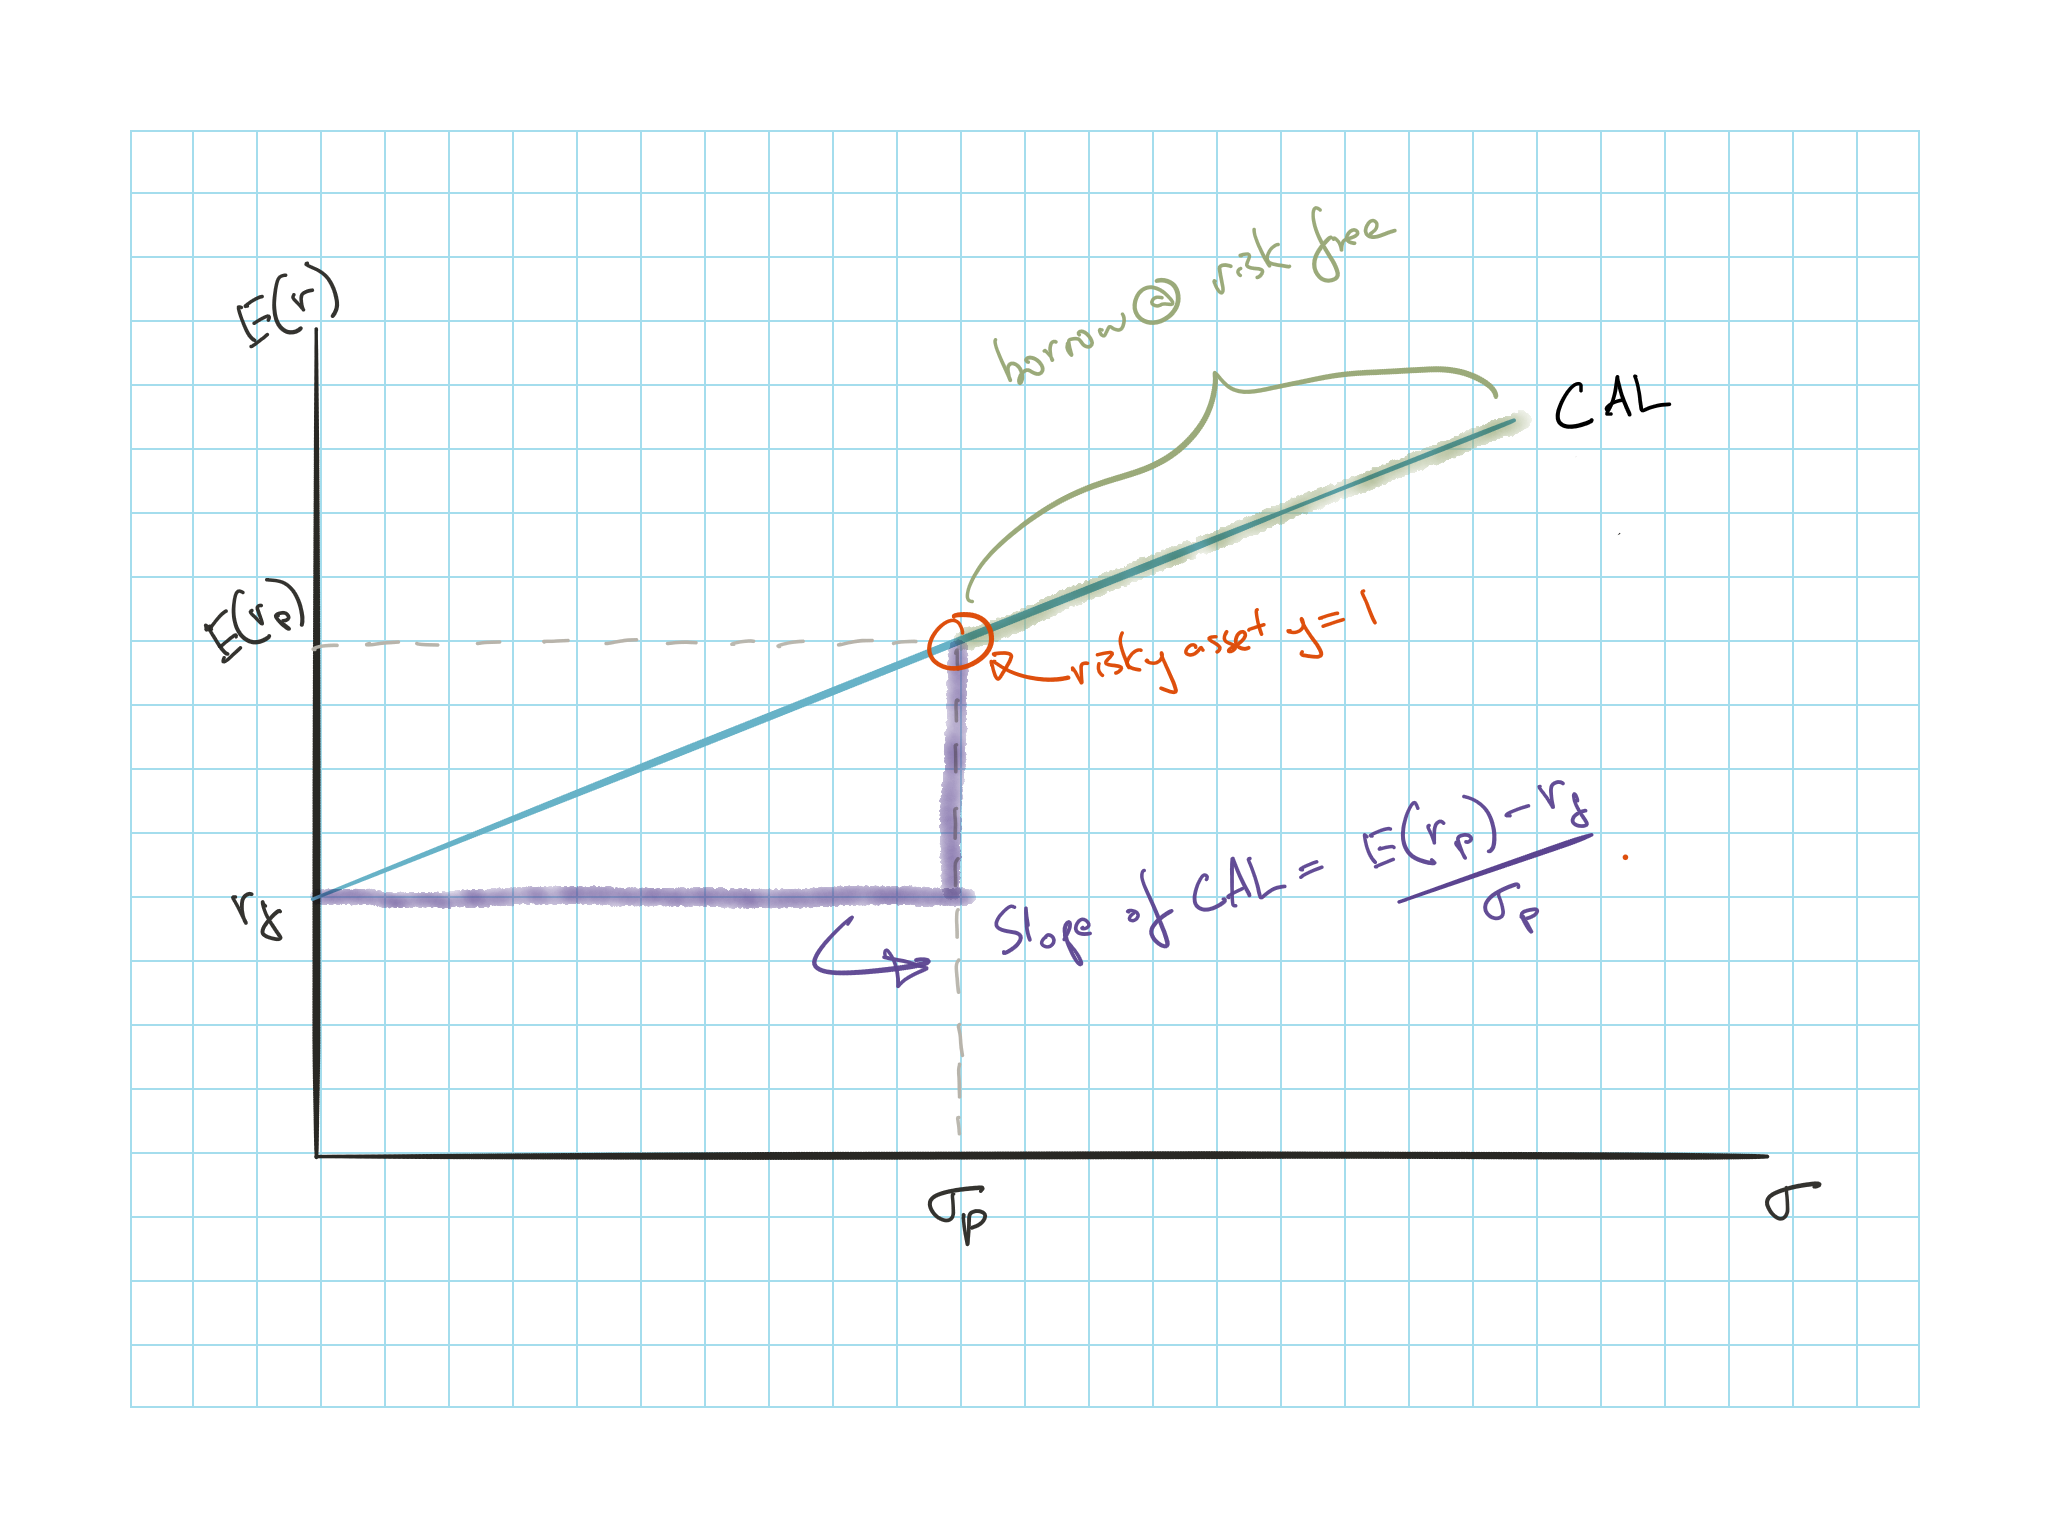
\includegraphics{figures/Exam 9 - 1.png}
\caption{alt text}
\end{figure}

Slop of CAL =
\(\left. \dfrac{\operatorname{E}[r_p] - r_f}{\sigma_p} \right \} \text{Sharpe Ratio} = \dfrac{\text{Incremental Return}}{\text{Unit of }\sigma}\)

CAL to the right of (\(\operatorname{E}[r_p]\), \(\sigma_p\)) is achieve
by borrowing at risk free rate

\begin{itemize}
\tightlist
\item
  If borrowing at risk free is not possible, the slope will be less
  steep = \(\dfrac{\operatorname{E}[r_p] - r_f^B}{\sigma_p}\) where
  \(r_f^B\) is the risk free rate we can borrow
\end{itemize}

\subsection{Risk Tolerance \& Asset
Allocation}\label{risk-tolerance-asset-allocation}

\textbf{Optimal Portfolio} maximizes investor utility with ratio \(y^*\)
on the risky asset

\(y^* = \dfrac{\operatorname{E}[r_p] - r_f}{A\sigma^2_p}\)

\begin{itemize}
\tightlist
\item
  Derived by setting the derivative of the utility equation = 0
\end{itemize}

 \textbf{Graphically} derive optimal risk portfolio

\begin{enumerate}
\def\labelenumi{\arabic{enumi})}
\item
  Plot \textbf{indifference curves}, which are curves that contain
  different portfolios that the investor is indifferent about, given the
  same \(U\) and \(A\)

  \begin{itemize}
  \tightlist
  \item
    Higher \(A\) produceds a steeper sloping indifference curve as an
    increase in \(\sigma\) requires higher \(\operatorname{E}[r]\) for
    investors that are more risk adverse
  \end{itemize}
\item
  Investor will pick the highest possible indifference curve that
  touches the CAL
\item
  Optimal portfolio is located at the intersection point of the CAL and
  the curve \textbf{tangential} to the CAL

  \begin{itemize}
  \tightlist
  \item
    As higher \(U\) will shift the curve upwards
  \end{itemize}
\end{enumerate}

\begin{figure}[htbp]
\centering
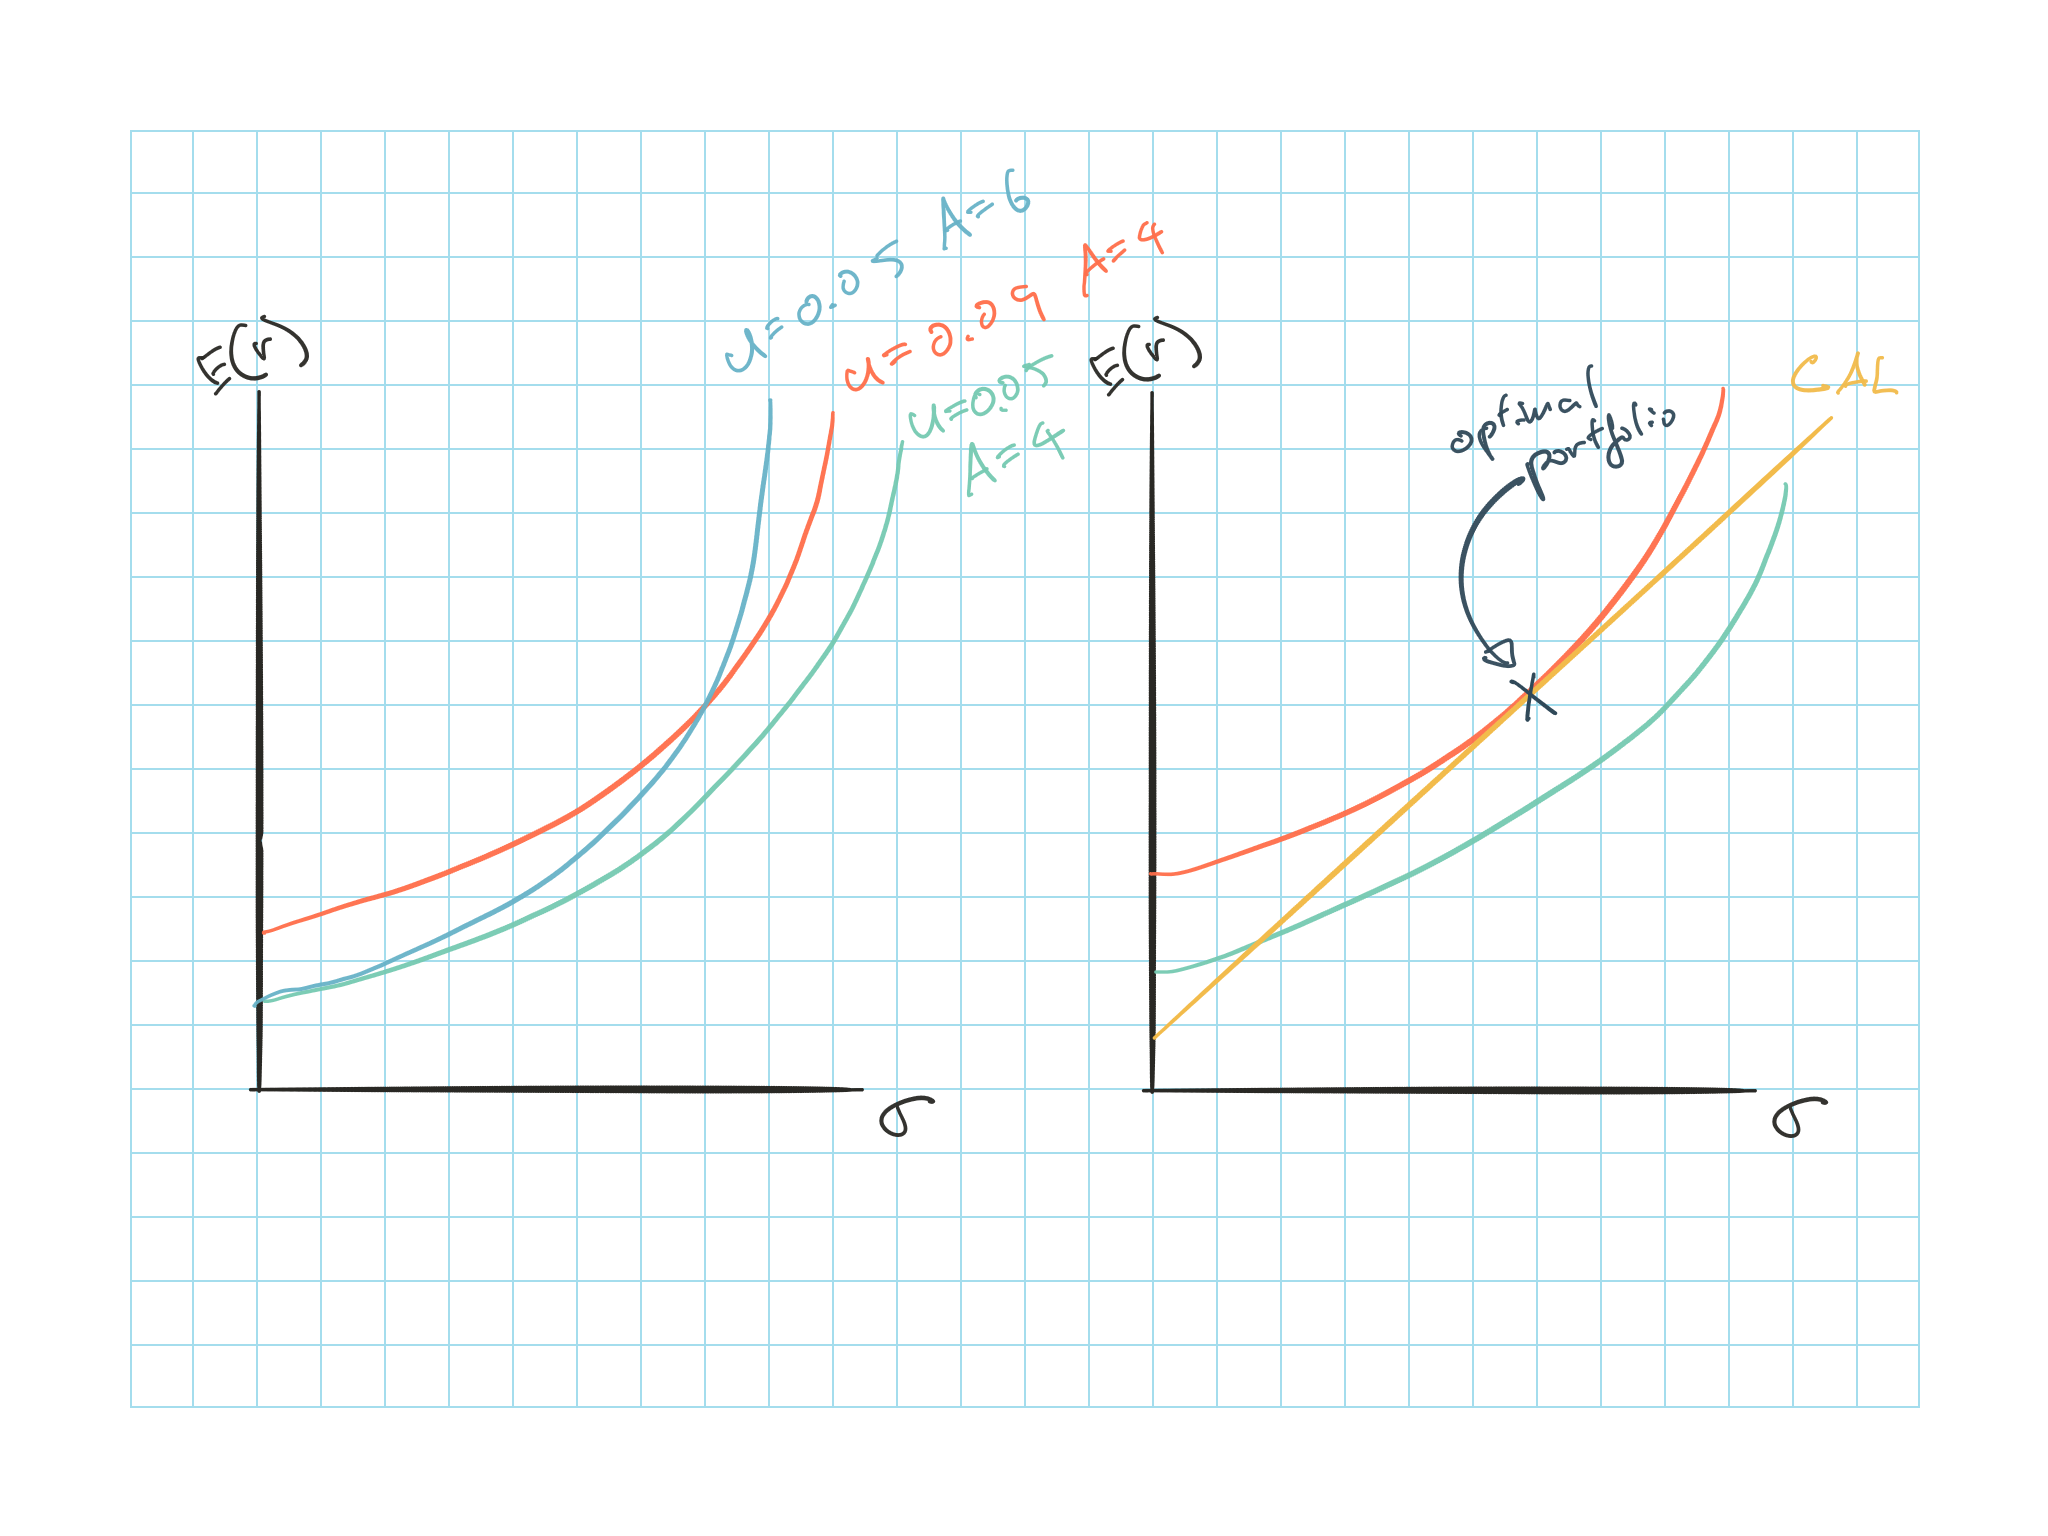
\includegraphics{figures/Exam 9 - 2.png}
\caption{alt text}
\end{figure}

\textbf{Proof} for \(y^*\) equation:

\(\begin{array}{lcccl}  U &= &\operatorname{E}[r_c] &- &\frac{1}{2}A\sigma_c^2 \\  U &= &y \operatorname{E}[r_p] + (1-y)r_f &- &\frac{1}{2}A(y\sigma_p)^2 \\  \frac{dU}{dy} &= &\operatorname{E}[r_p] - r_f &- & A y \sigma^2_p \\  0 &= &\operatorname{E}[r_p] - r_f &- & A y \sigma^2_p \\  A y \sigma^2_p &= &\operatorname{E}[r_p] - r_f \\  y &= &\dfrac{\operatorname{E}[r_p] - r_f}{A \sigma^2_p } \\ \end{array}\)

\subsection{Non Normal Returns}\label{non-normal-returns}

Analysis so far used the \(\sigma\) as the measure of risk and it
assumes return \(\sim N(\mu, \sigma)\)

If returns are more heavy tailed than normal \(\Rightarrow\) Reduce
allocation to the risky portfolio compared to the indication above

\subsection{Capital Market Line}\label{capital-market-line}

\textbf{Capital Market Line}\\
CAL that uses a passive portfolio as the risky portfolio

\textbf{Passive} strategy for risky portfolio:

\begin{itemize}
\tightlist
\item
  Based on a selected benchmark portfolio
\item
  Significant cheaper than an active strategy
\item
  Free rider benefit: Assets should be fairly priced as mispricings
  should disappear from investors implementing the active strategy
\end{itemize}

\textbf{Active} strategy is to determine the risky portfolio with
security analysis

\section{Past Exam Questions}\label{past-exam-questions}

 2003, Q3 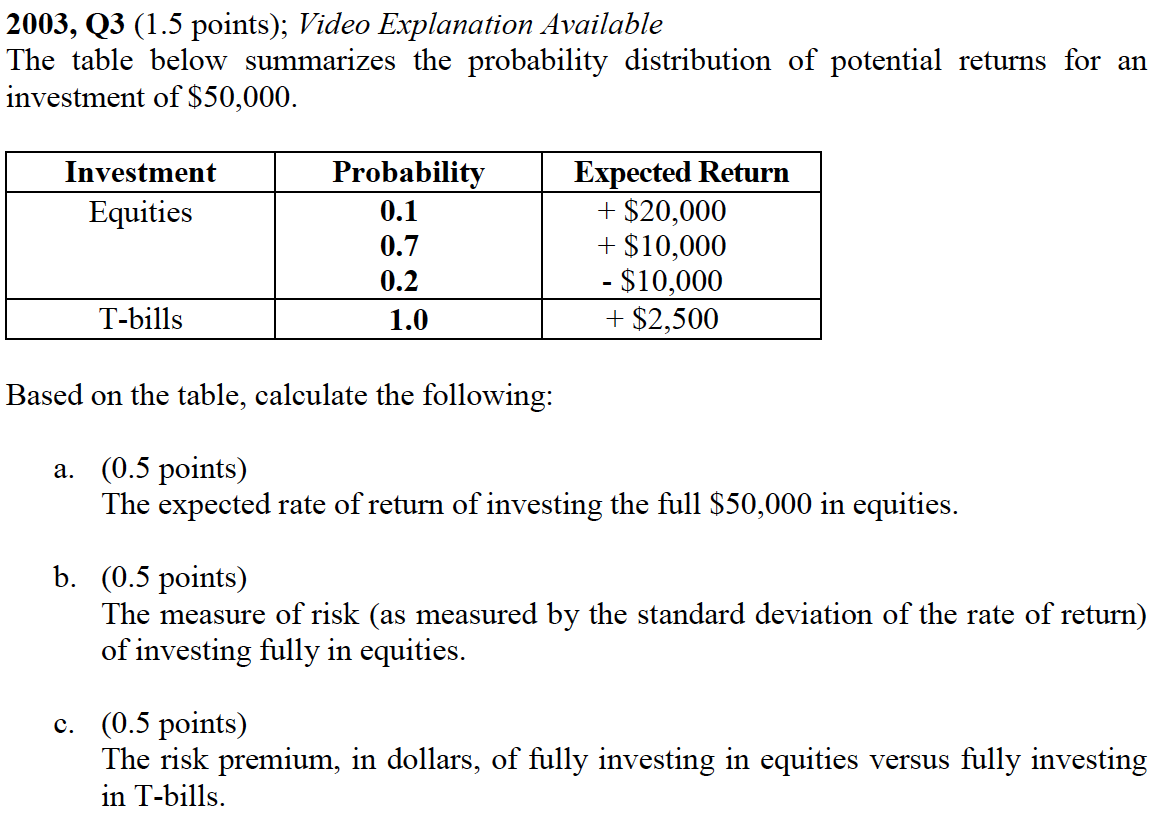
\includegraphics{questions/2003-3Q.png}
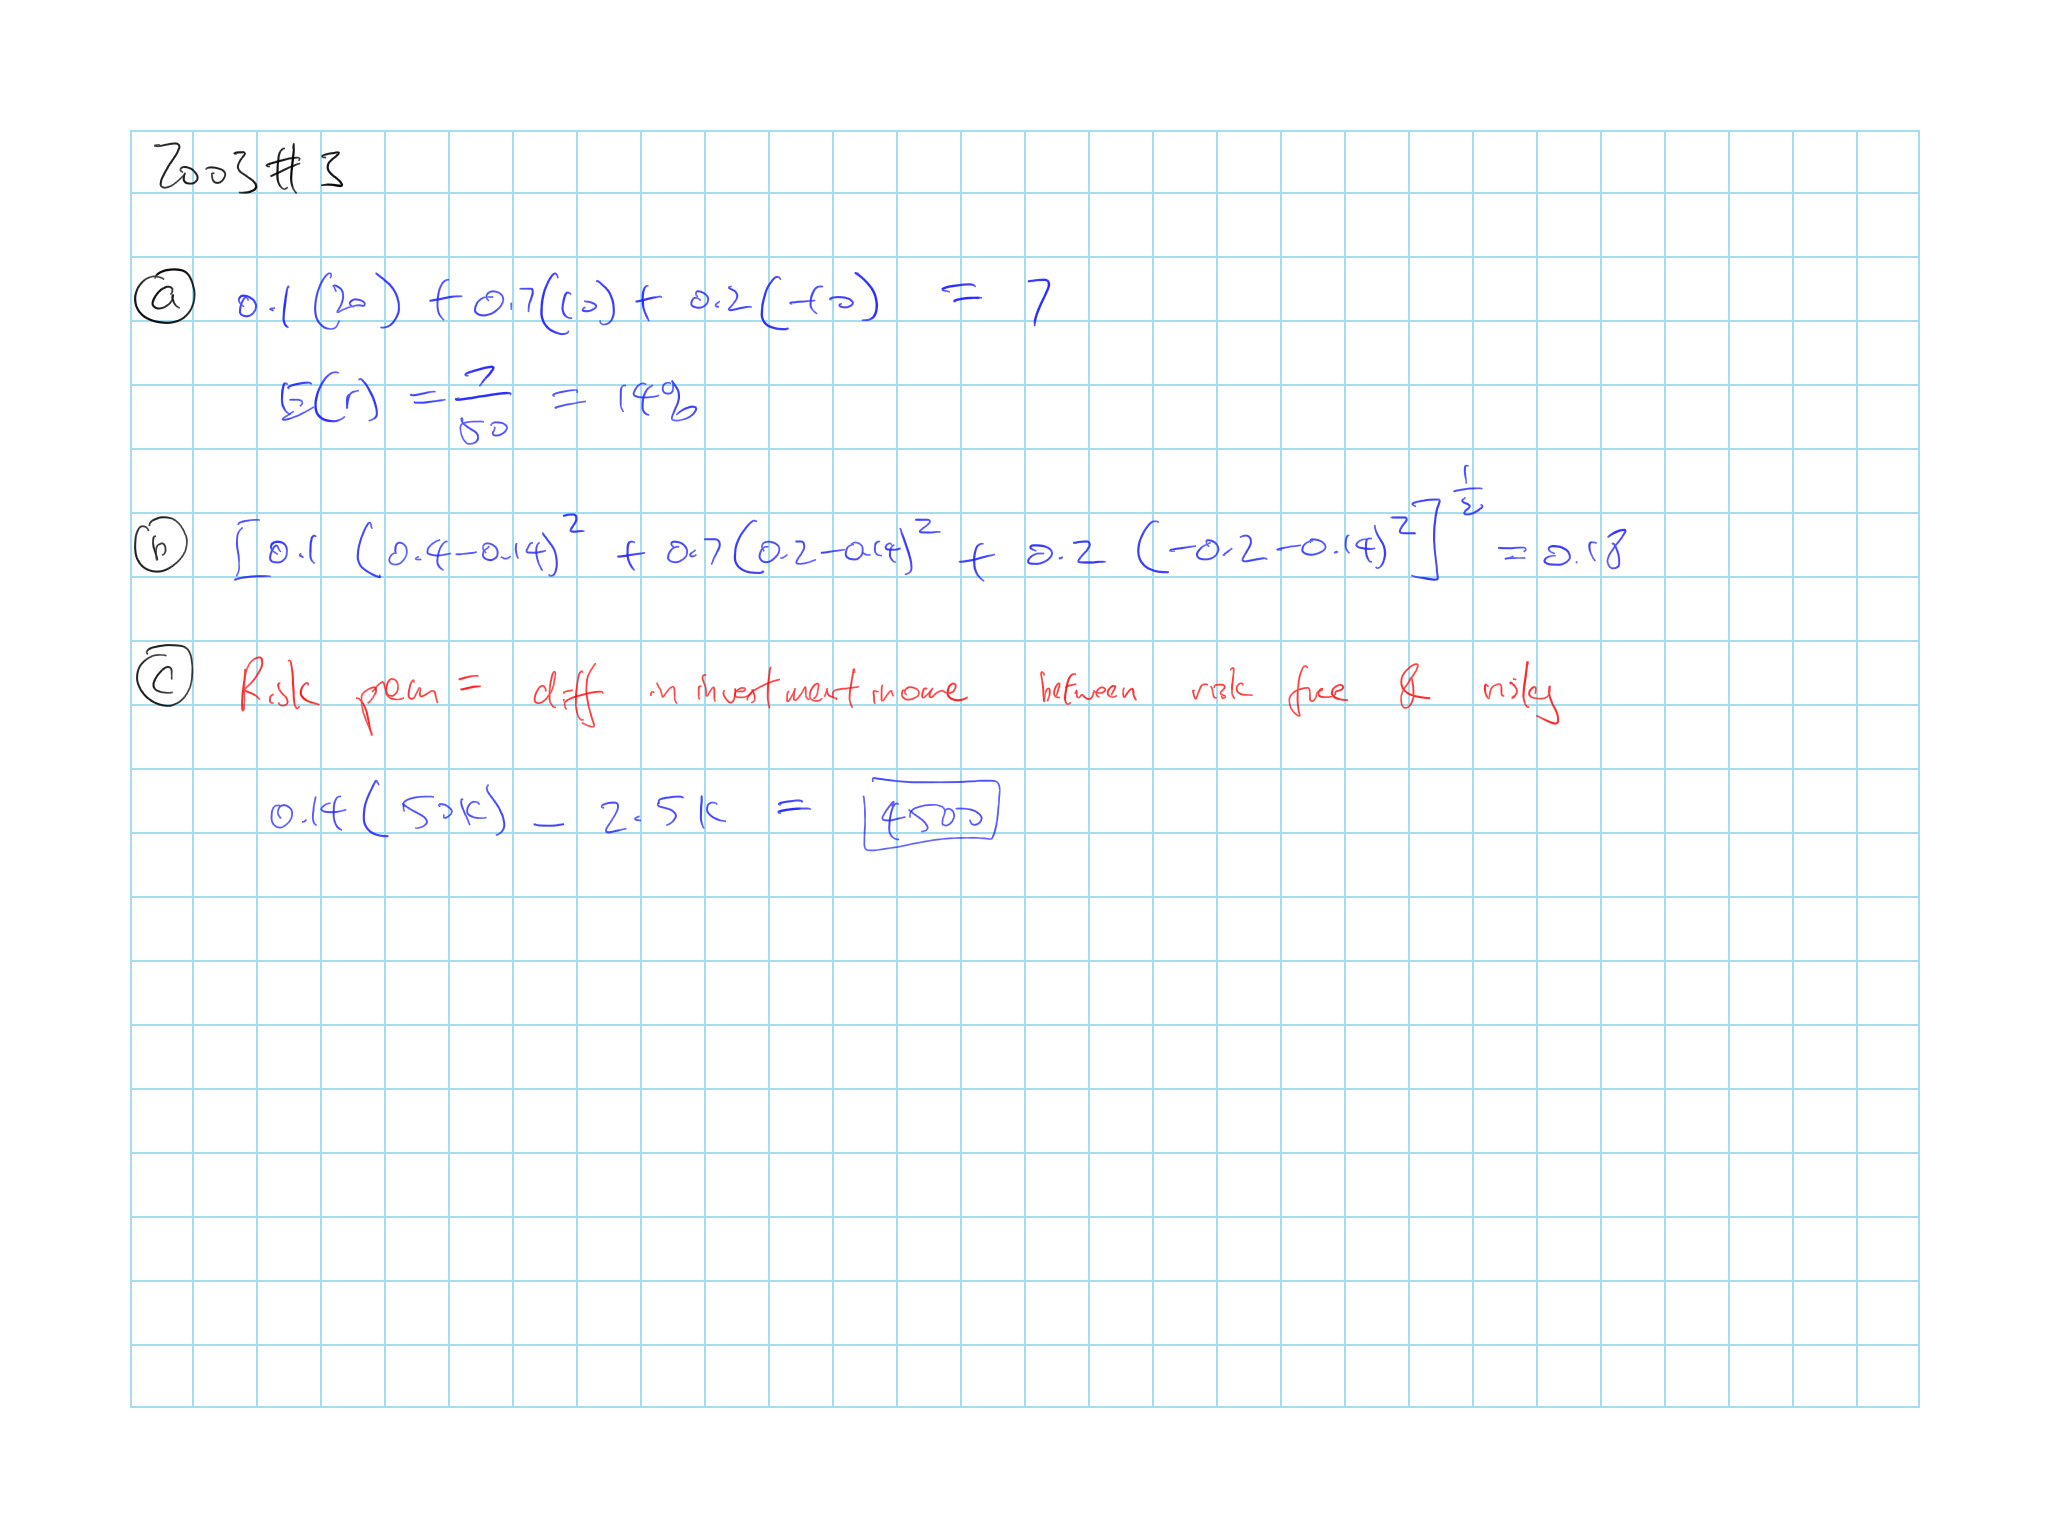
\includegraphics{questions/2003-3A.png}

 2003, Q4 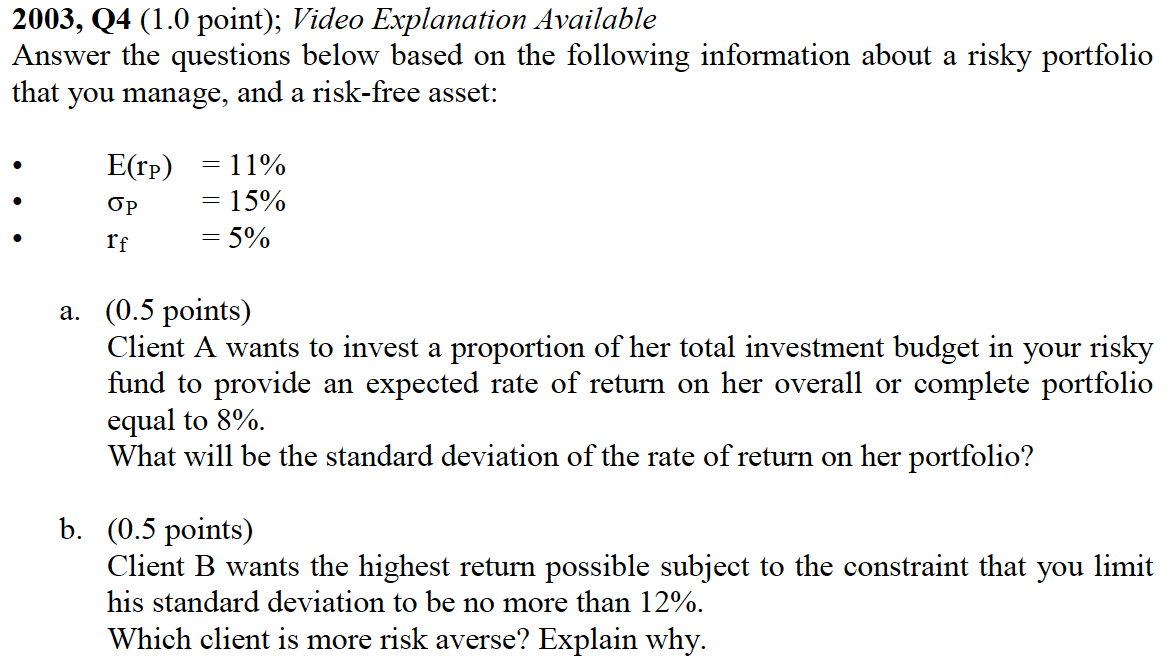
\includegraphics{questions/2003-4Q.png}
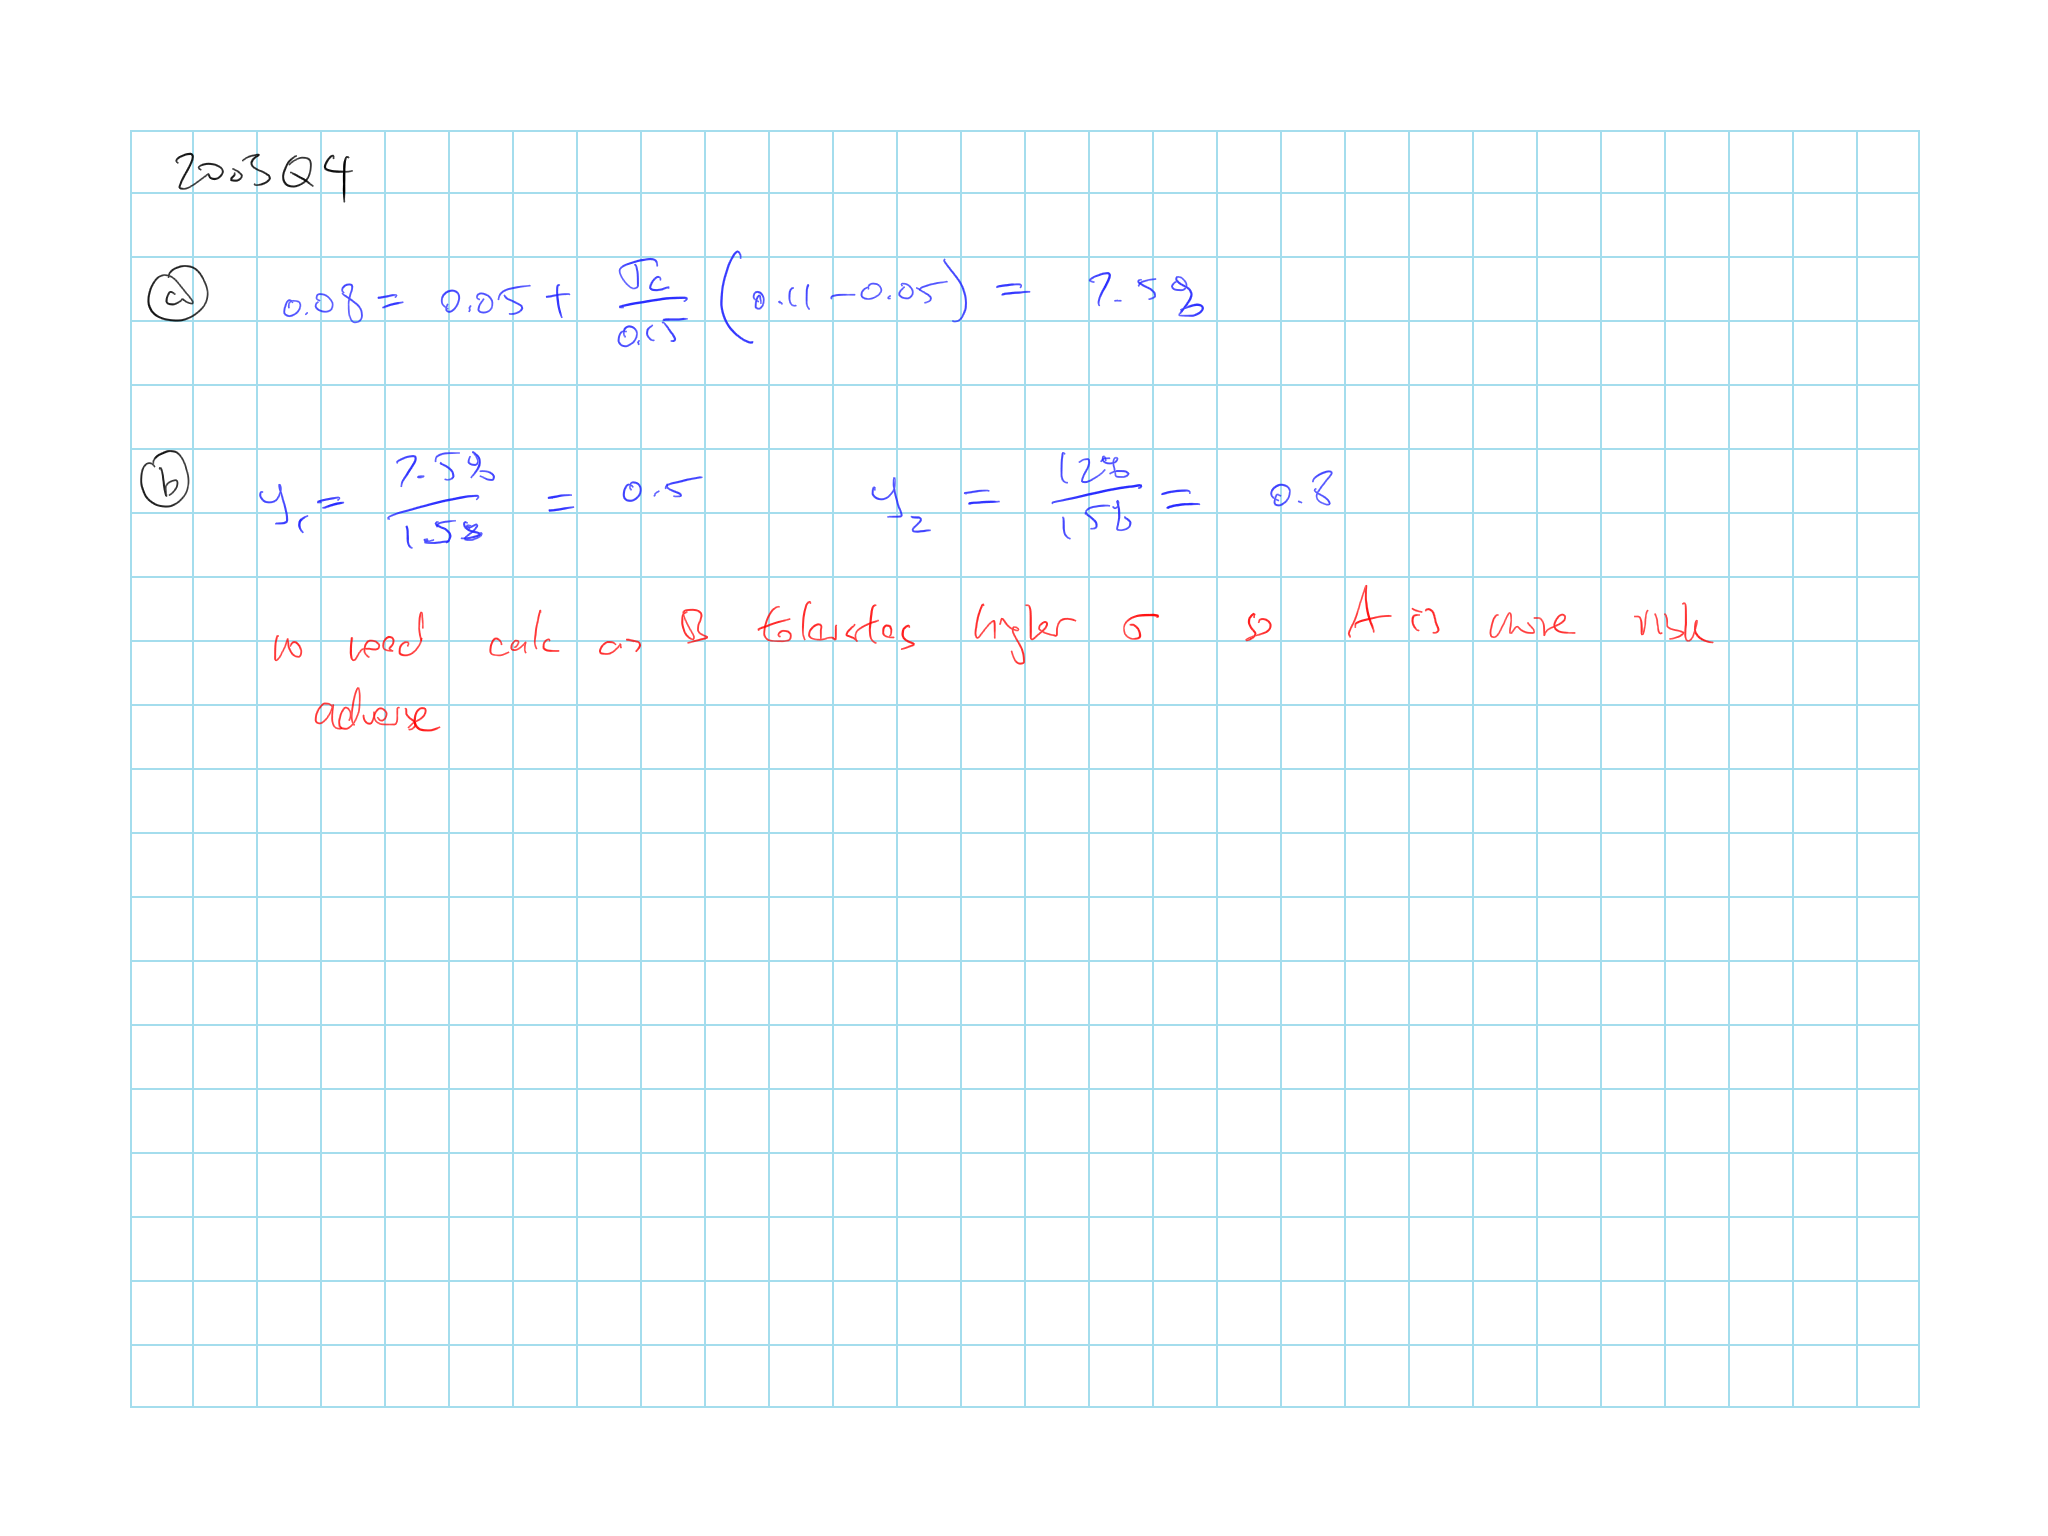
\includegraphics{questions/2003-4A.png}

 2009, Q1 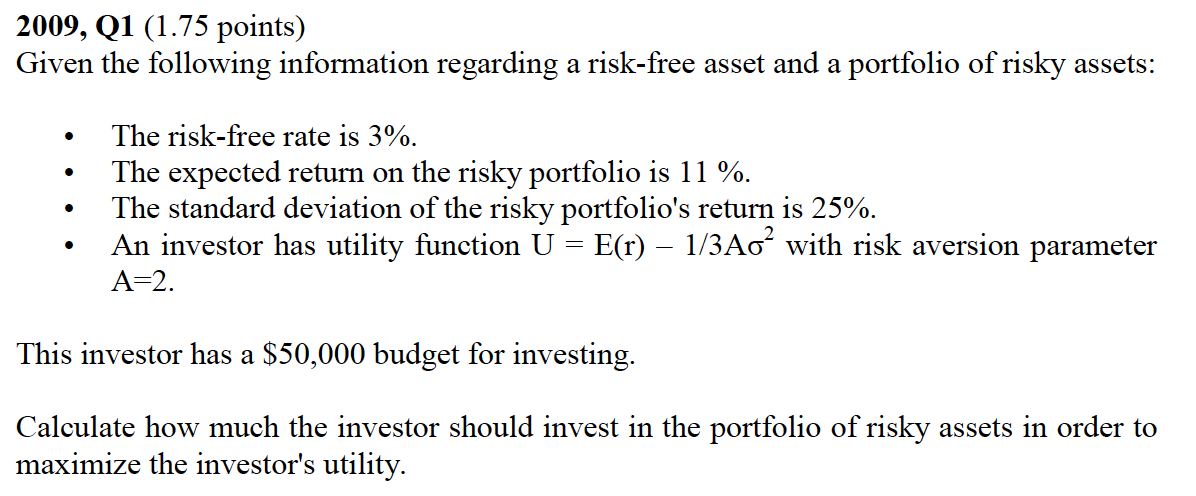
\includegraphics{questions/2009-1Q.png}
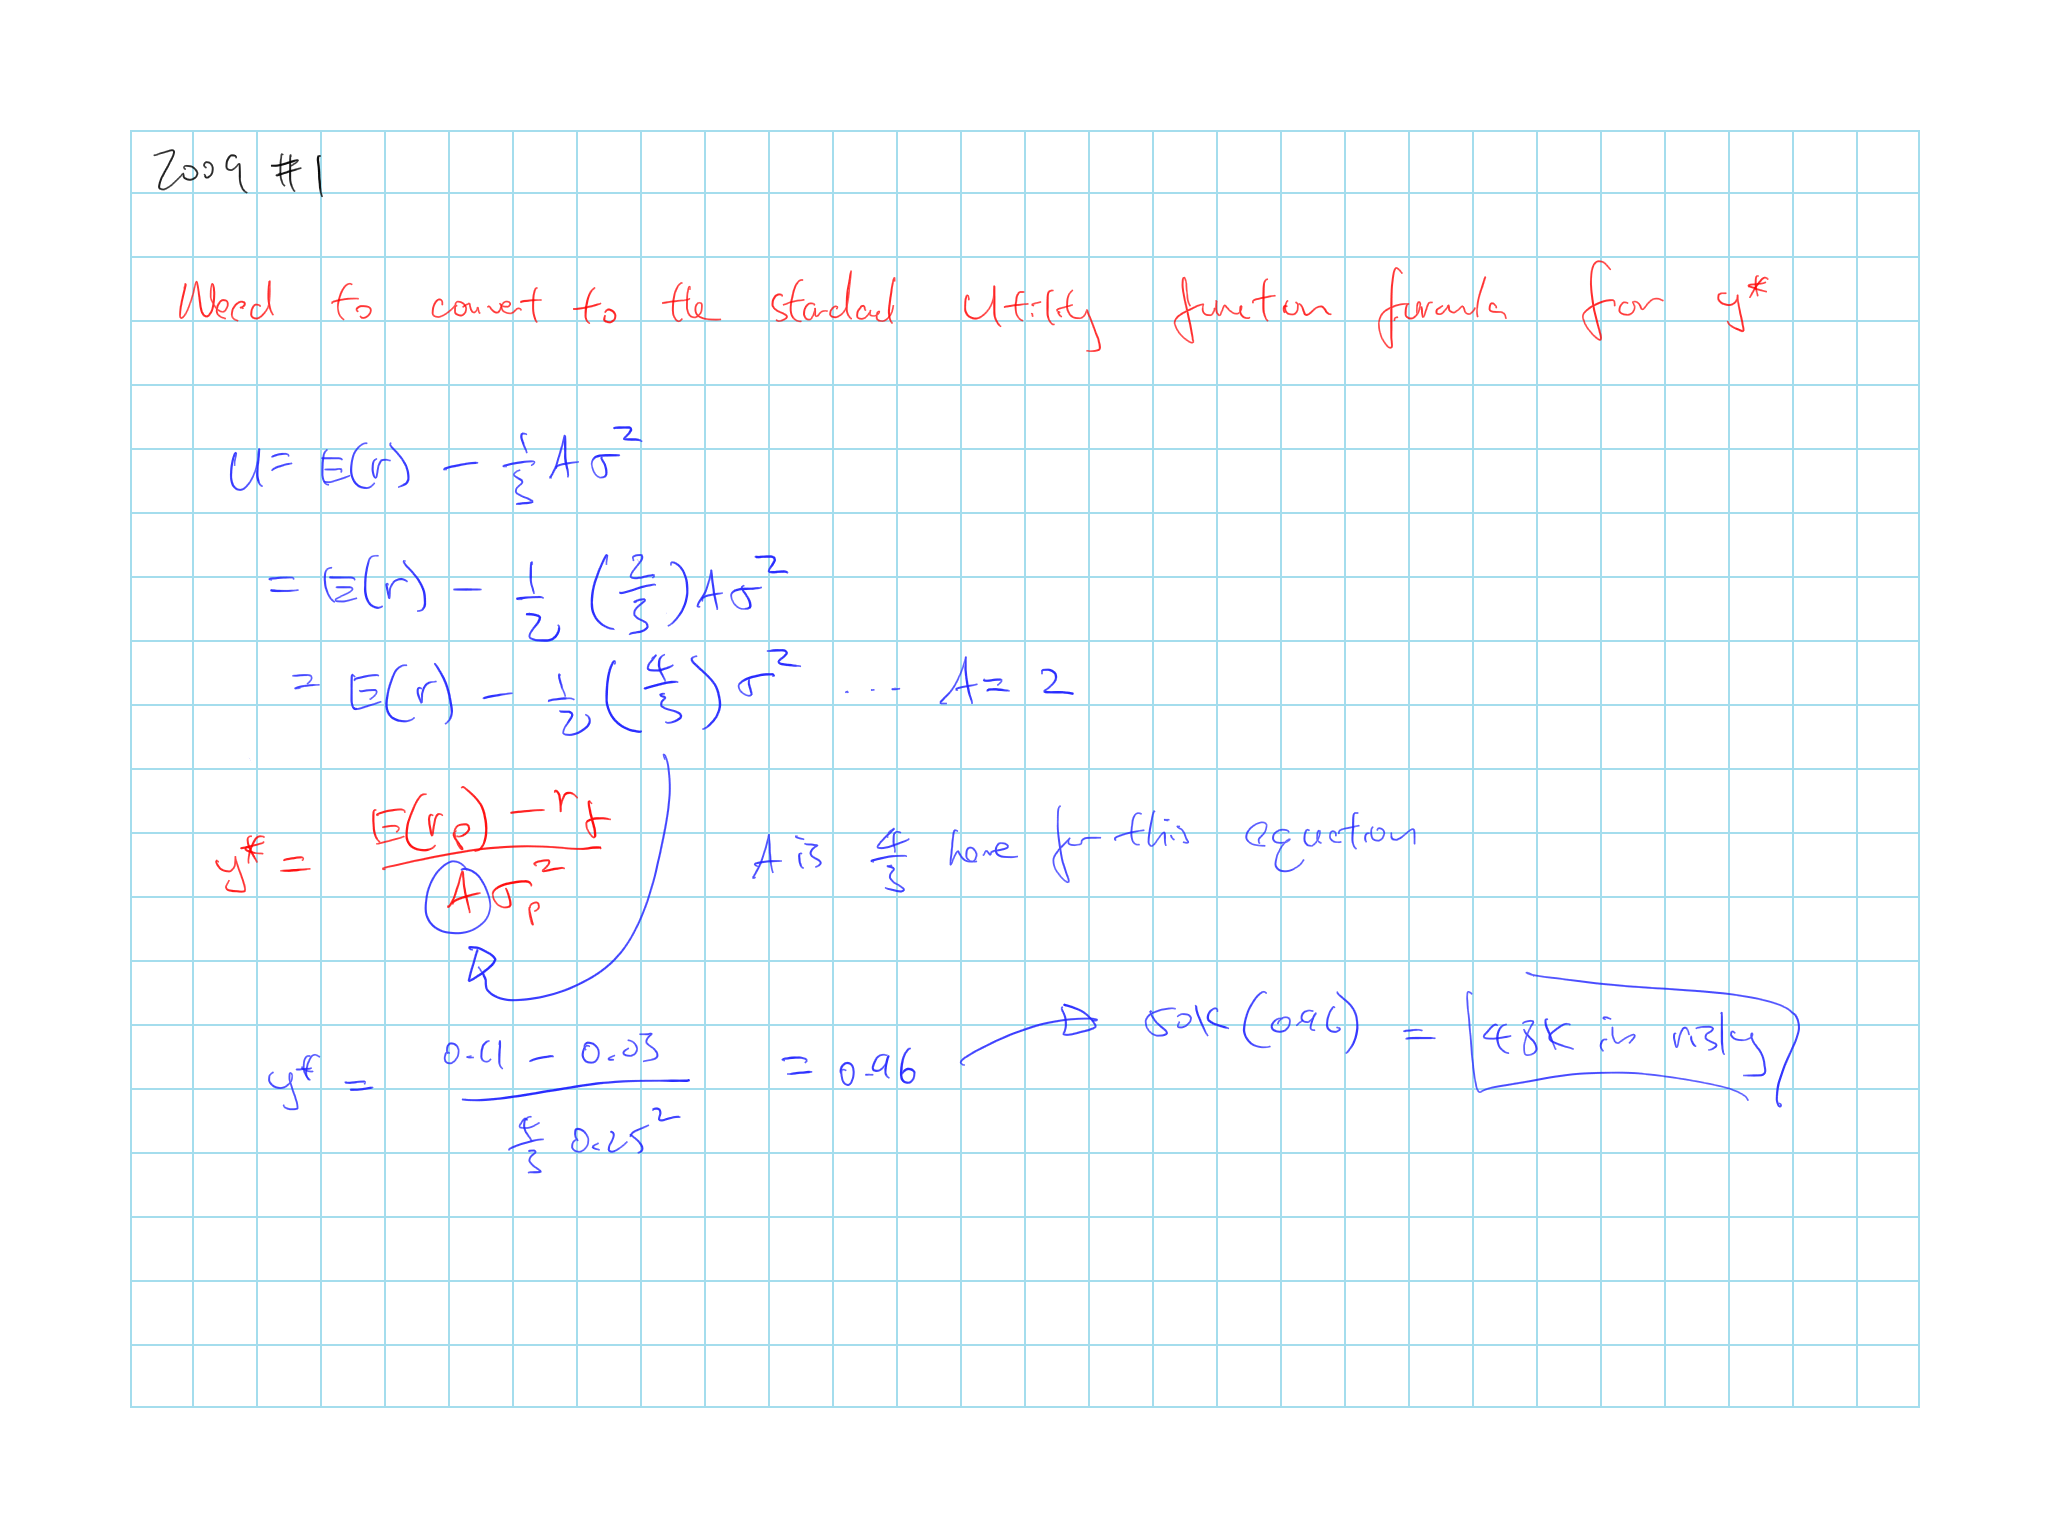
\includegraphics{questions/2009-1A.png}

 2011, Q1 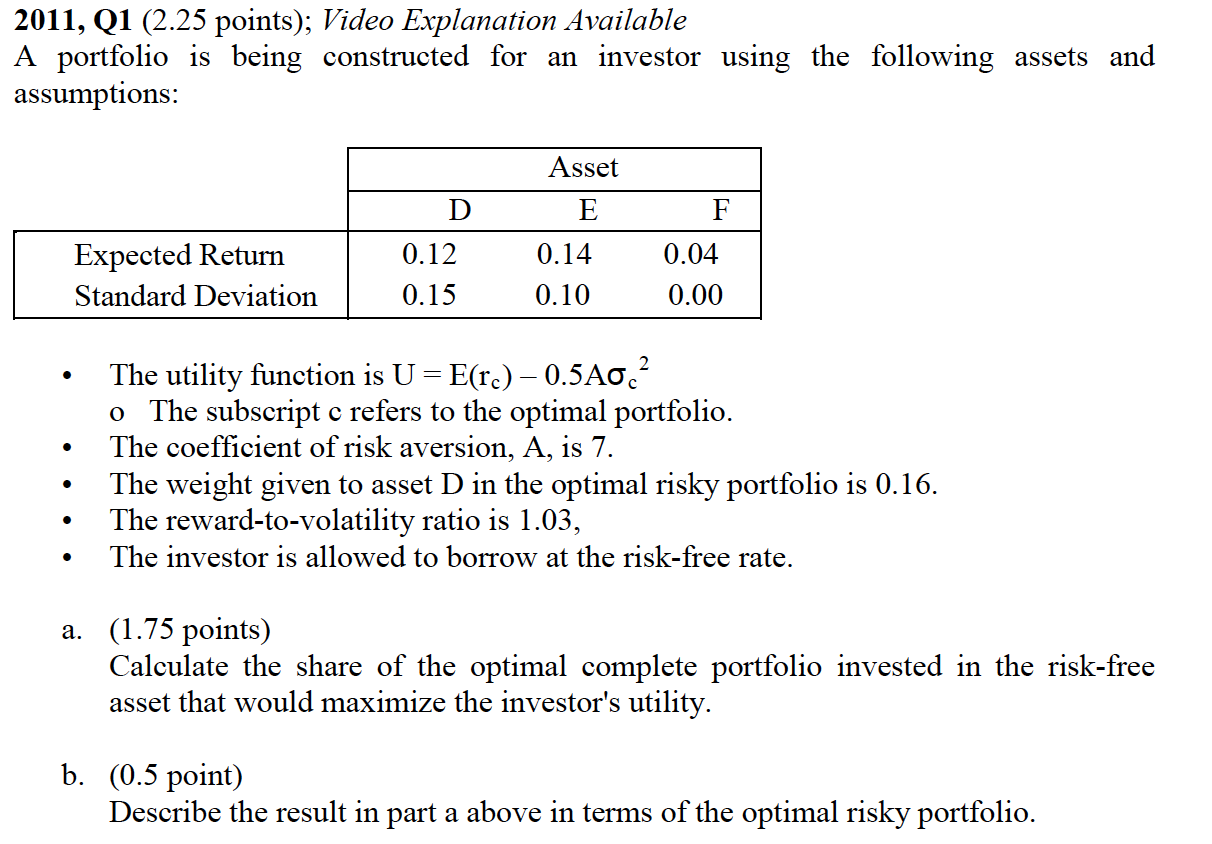
\includegraphics{questions/2011-1Q.png}
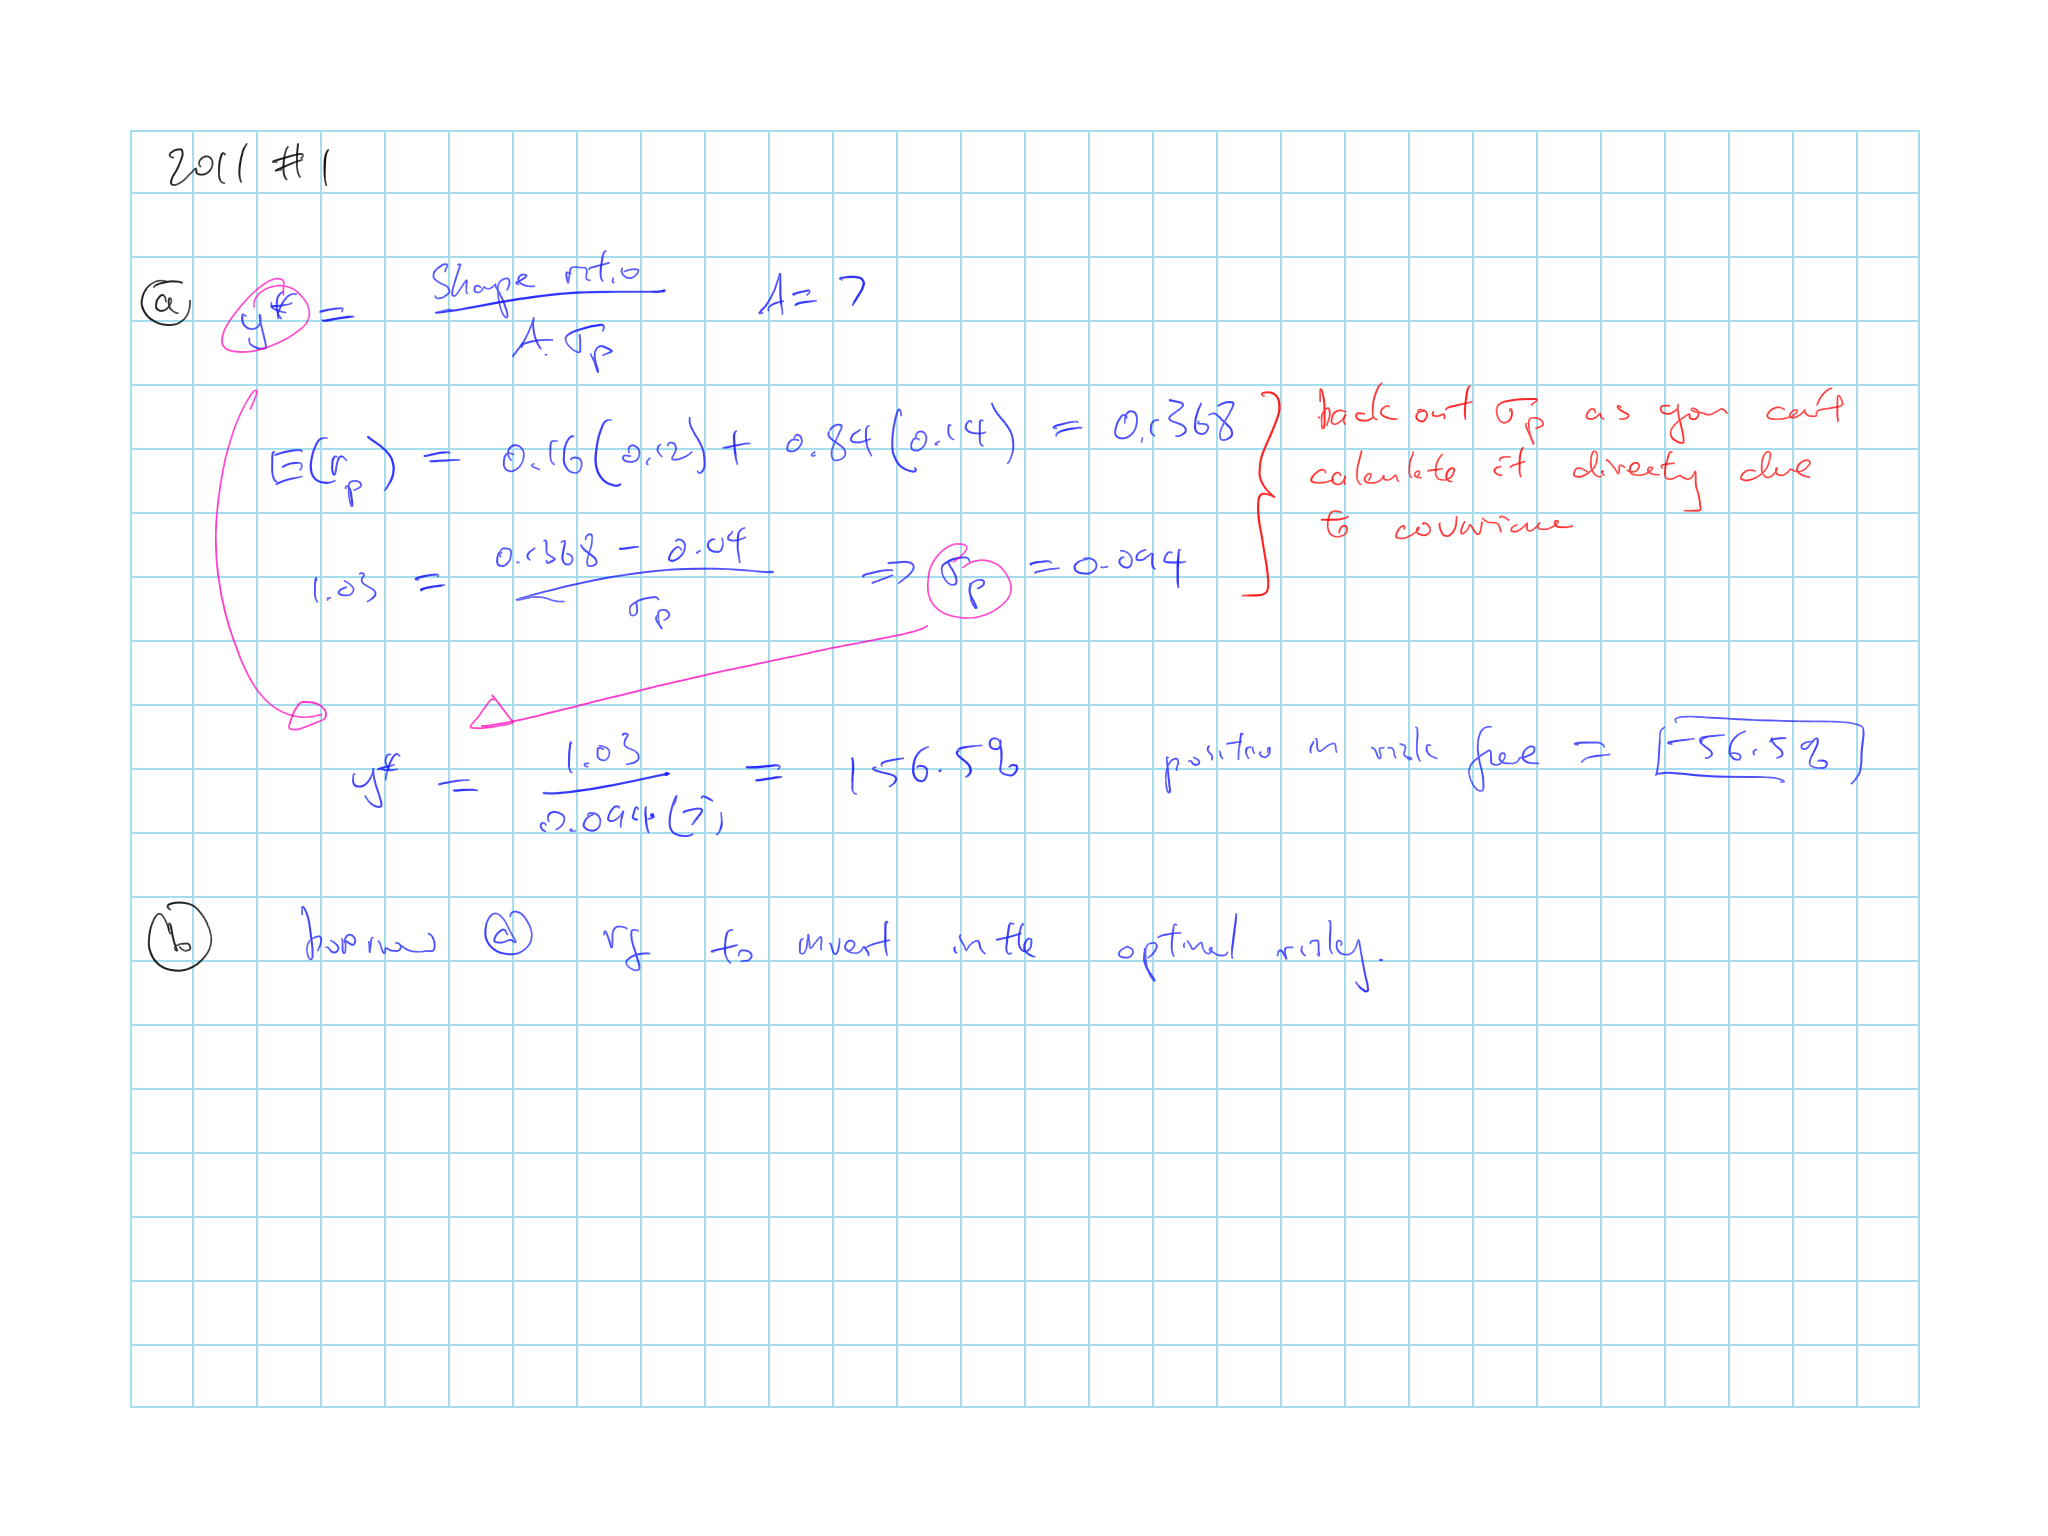
\includegraphics{questions/2011-1A.png}

 2012, Q1 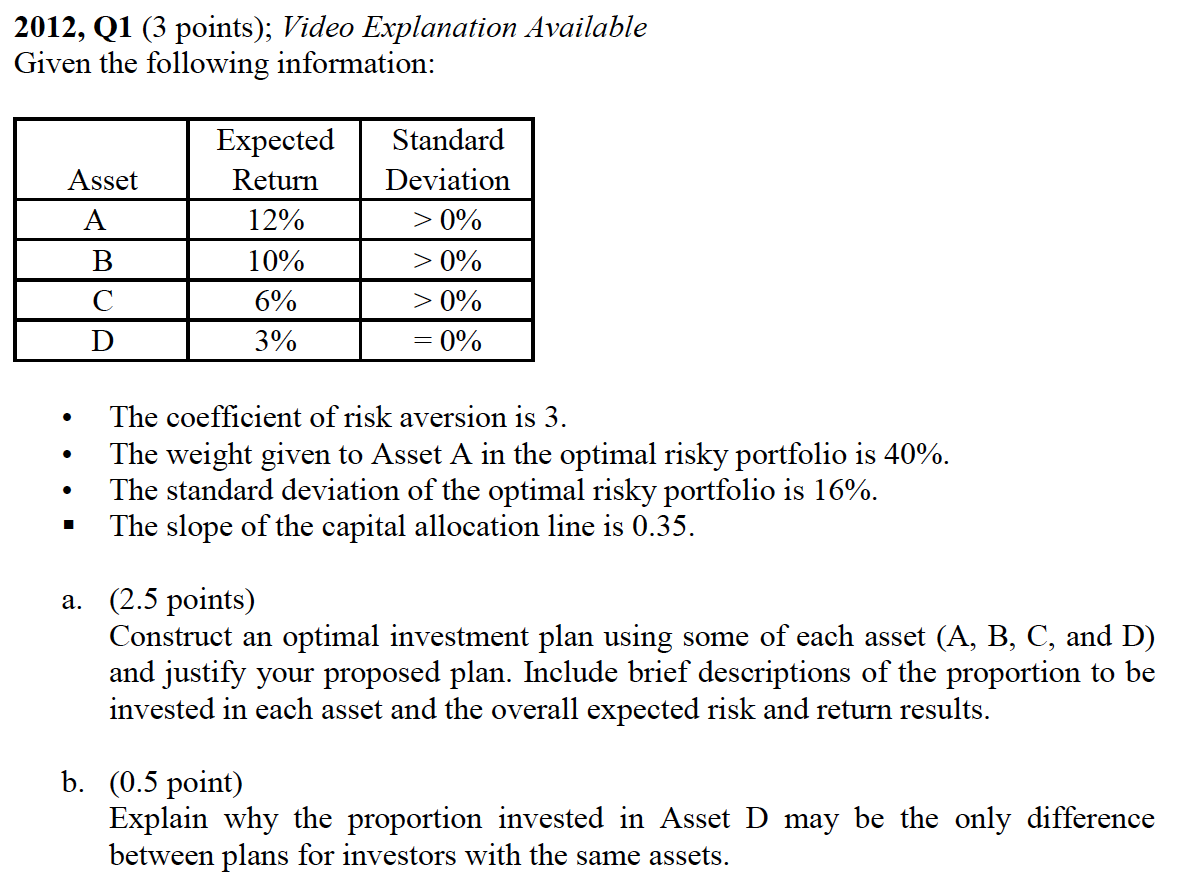
\includegraphics{questions/2012-1Q.png}
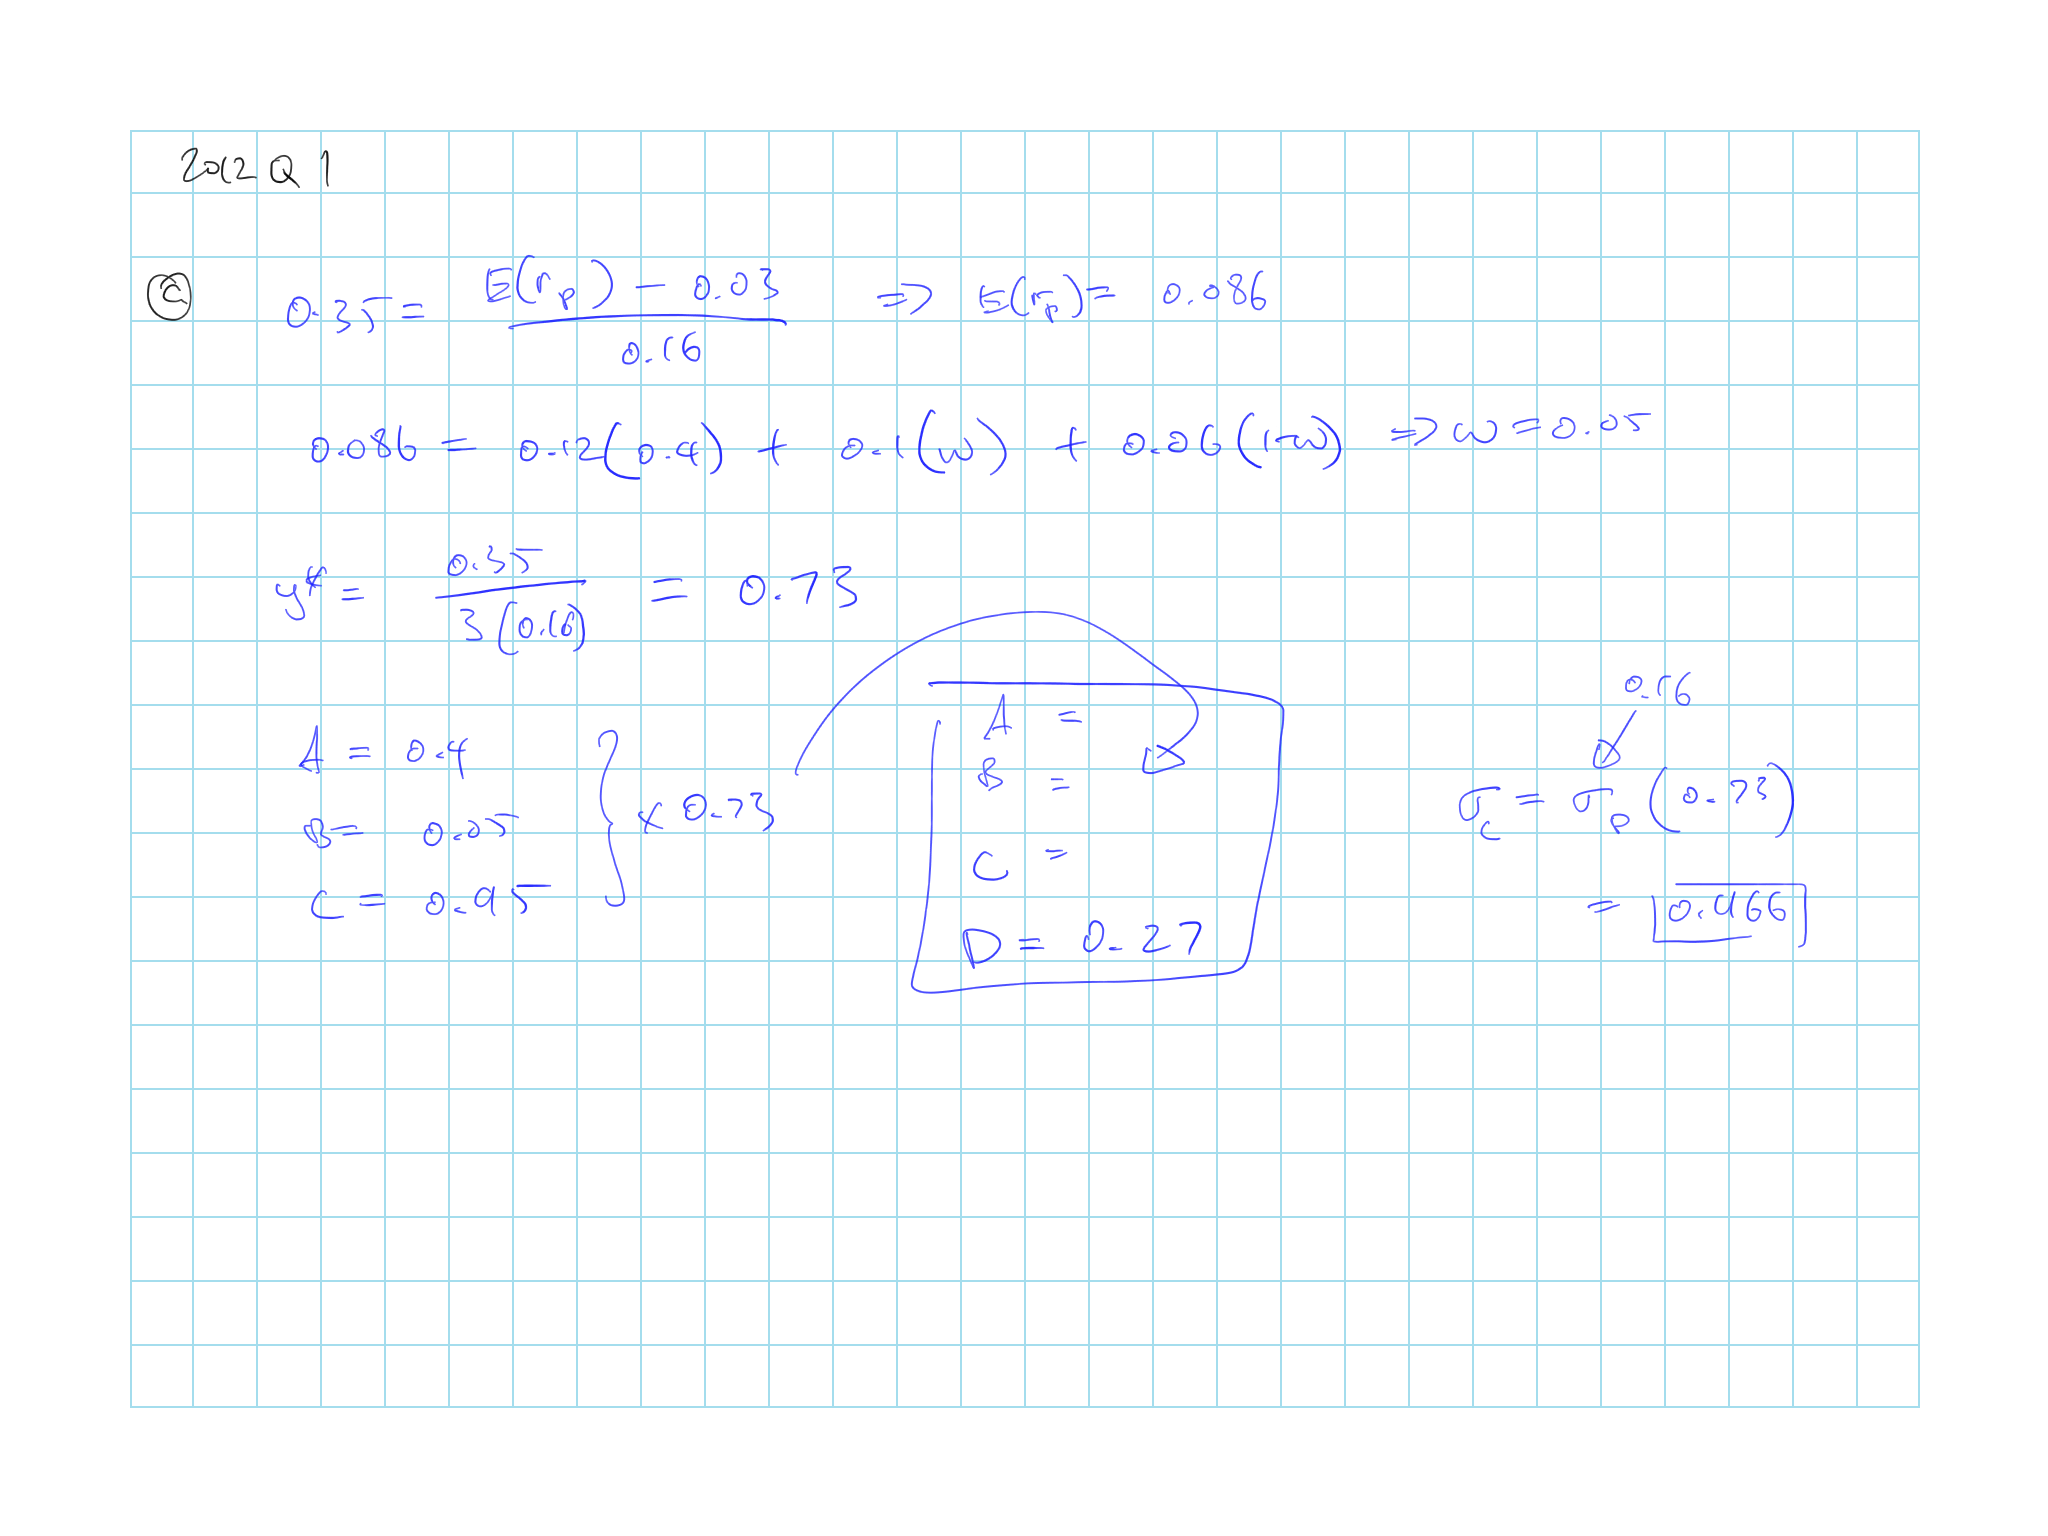
\includegraphics{questions/2012-1A.png}

\chapter{A2 BKM7: Optimal Risky
Portfolios}\label{a2-bkm7-optimal-risky-portfolios}

Z. Bodie, A. Kane, A. Marcus

\section{Cliff's Summary}\label{cliffs-summary-1}

\textbf{Total Variance of a Portfolio of Equally Weighted Assets}

\(\sigma^2_p = \underbrace{\overbrace{\dfrac{\bar{\sigma}^2}{n}}^{\lim \limits_{n \rightarrow \infty} \rightarrow 0}}_{\text{Firm Risk}} + \underbrace{\dfrac{n-1}{n}\bar{\operatorname{Cov}}}_{\text{Systematic Risk}}\)

\textbf{For 2 risky asset}

\(\operatorname{E}[r_p] = w_D \operatorname{E}[r_D] + w_E \operatorname{E}[r_E]\)

\(\sigma^2_p = w^2_D \cdot \sigma^2_D + w^2_E \cdot \sigma^2_E + 2 \cdot w_D \cdot w_E \cdot \operatorname{Cov}(r_D, r_E)\)

Weights for the minimum variance portfolio

\(w_D^{Min} = \dfrac{\sigma^2_E - \operatorname{Cov}(r_D, r_E)}{\sigma^2_E + \sigma^2_D - 2\cdot\operatorname{Cov}(r_D, r_E)}\)

Know the shape of the \protect\hyperlink{ptf-op-set}{portfolio
opportunity set} for different \(\rho\)

\textbf{For 2 risky asset and risk free}

Optimal Risky Portfolio: Available portfolio with highest Sharpe ratio

Weights of the optimal risky portfolio:

\(w_D = \dfrac{\operatorname{E}[R_D]\sigma^2_E - \operatorname{E}[R_E] \operatorname{Cov}(r_D, r_E)}{\operatorname{E}[R_D]\sigma^2_E + \operatorname{E}[R_E]\sigma^2_D - \left( \operatorname{E}[R_D] + \operatorname{E}[R_E] \right) \operatorname{Cov}(r_D, r_E)}\)

\begin{itemize}
\tightlist
\item
  \(R_D = r_D - r_f\) = XS return over risk free
\end{itemize}

\begin{center}\rule{0.5\linewidth}{\linethickness}\end{center}

Markowitz Portfolio

\protect\hyperlink{sep-prin}{Seperation principle}

Asset allocation vs security allocation

Risk pooling (does not reduce risk) vs risk sharing

\begin{itemize}
\tightlist
\item
  Caveat of risk sharing
\end{itemize}

Time diversification is not true

\subsection{Types of Exam Questions}\label{types-of-exam-questions-1}

{Haven't done TIA practice questions}

\textbf{Plug and play}

\begin{itemize}
\tightlist
\item
  2000, Q8: minimum variance expected return by calculating the weight
\end{itemize}

\textbf{Weights Calculation}

\begin{itemize}
\tightlist
\item
  \protect\hyperlink{2003-5}{2003, Q5}: Weights for risky and risk free
  and CAL
\item
  2005, Q5: optimal risky portfolio and special case with
  \(\rho = -1 or 1\)
\item
  2006, Q5: weight for assets in optimal risky
\item
  2007, Q2: optimal risky weights and complete portfolio weights
\item
  \(\star\) 2008, Q1: optimal risky and complete ptf and rebalance
\item
  2009, Q2: optimal risky portfolio and sharpe ratio
\item
  2014, Q5: optimal complete portfolio return and \(\sigma_c\)
\end{itemize}

\textbf{Concepts}

\begin{itemize}
\tightlist
\item
  2001, Q10: Draw CML and efficient frontier
\item
  2002, Q7: Draw portfolio opportunity set for \(\rho = -1\) and
  \(\sigma\) when \(\rho = 1\)
\item
  2002, Q13: Fallacy of time diversification
\item
  2003, Q7: Efficient frontier
\item
  2004, Q4: seperation principle; draw CAL, eff frontier; indifference
  curve
\item
  2005, Q6: draw ptf opporunity set
\item
  2007, Q3: fallacy of time diversification
\item
  2013, Q3: risk sharing and pooling in insurance
\end{itemize}

\textbf{Other}

\begin{itemize}
\tightlist
\item
  \(\star\) \protect\hyperlink{2009-3}{2009, Q3}: systematic risk,
  variance
\item
  \(\star\) \protect\hyperlink{2015-1}{2015, Q1}: \(A\), \(\rho\), and
  backout \(A\)
\end{itemize}

\section{Diversification and Portfolio
Risk}\label{diversification-and-portfolio-risk}

2 categories of risk:

\begin{itemize}
\item
  \textbf{Market/ Systematic/ Nondiversifiable Risk}: Risk that can no
  be diversified away
\item
  \textbf{Unique/ Firm-Specific/ Nonsystematic/ Diversifiable}: Portion
  of the risk that can be eliminated via diversification
\end{itemize}

\begin{figure}[htbp]
\centering
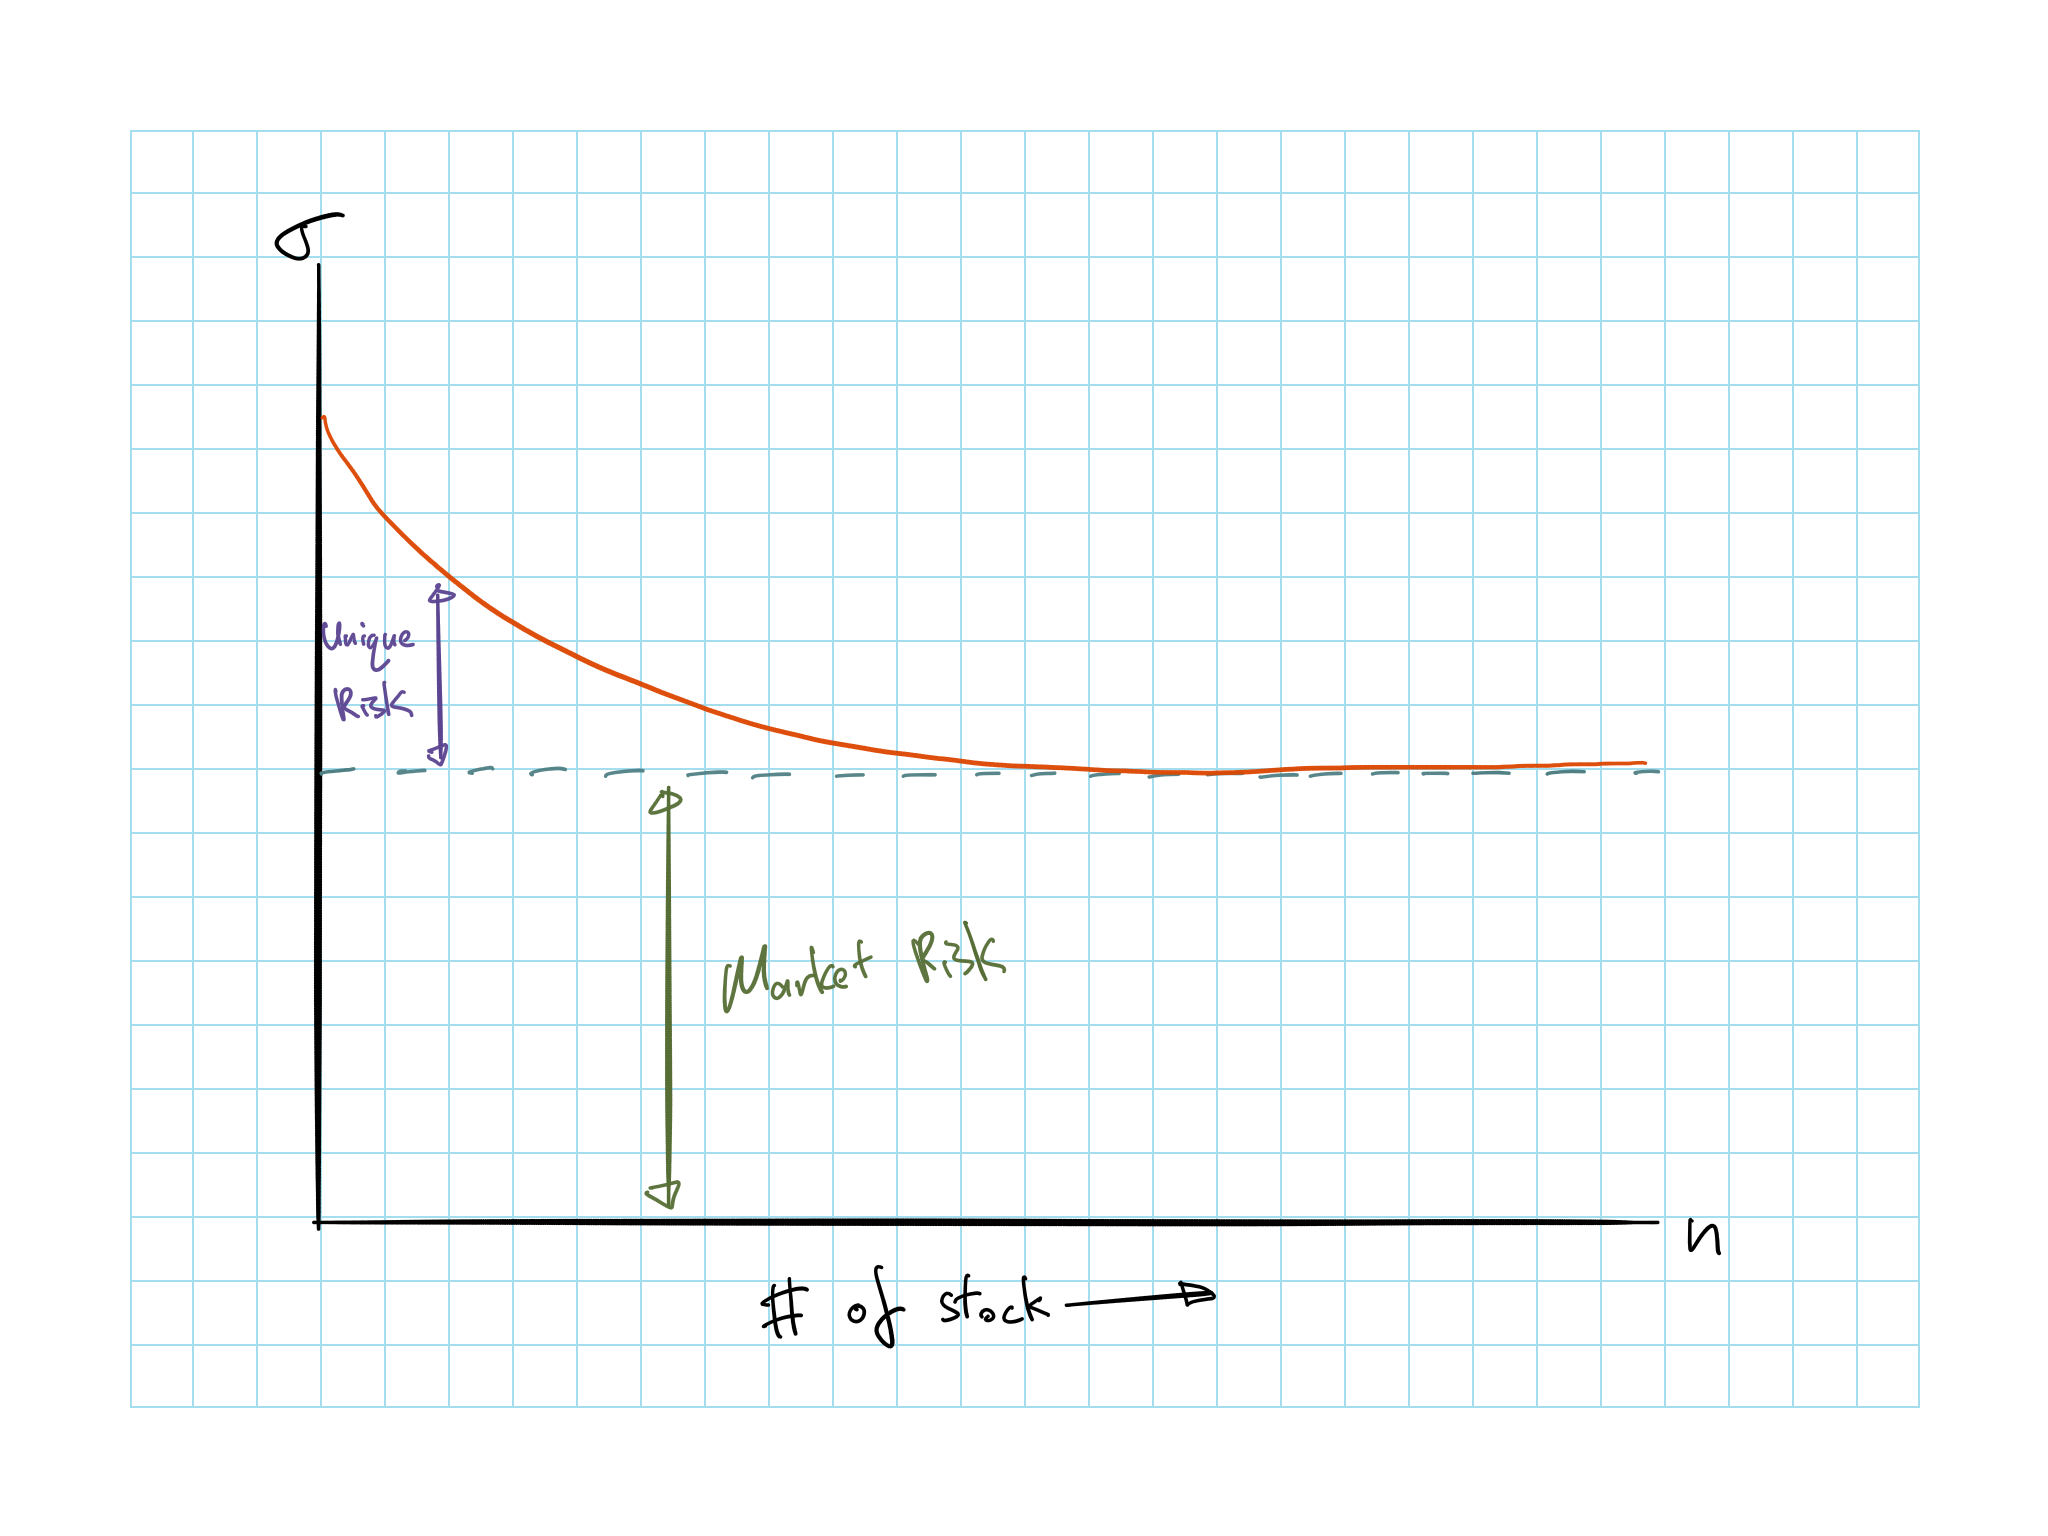
\includegraphics{figures/Exam 9 - 3.png}
\caption{alt text}
\end{figure}

\textbf{Total Variance of a Portfolio of Equally Weighted Assets}

\(\sigma^2_p = \underbrace{\overbrace{\dfrac{\bar{\sigma}^2}{n}}^{\lim \limits_{n \rightarrow \infty} \rightarrow 0}}_{\text{Firm Risk}} + \underbrace{\dfrac{n-1}{n}\bar{\operatorname{Cov}}}_{\text{Systematic Risk}}\)

\begin{itemize}
\item
  Systematic risk remains even as \(n \rightarrow \infty\)
\item
  Formula assumes each of the \(n\) securities have the same \(\sigma\)
  and \(\bar{\operatorname{Cov}}\) with each other
\item
  For a diversified portfolio the contribution to portfolio risk will
  only depends on the covariance of the security's return with other
  securities
\end{itemize}

\section{Portfolios of 2 Risky
Assets}\label{portfolios-of-2-risky-assets}

\textbf{Efficient Diversification}\\
Weights of risky assets that would produce lowest risk level for the
risky portfolio P

\(\operatorname{E}[r_p] = w_D \operatorname{E}[r_D] + w_E \operatorname{E}[r_E]\)

\(\sigma^2_p = w^2_D \cdot \sigma^2_D + w^2_E \cdot \sigma^2_E + 2 \cdot w_D \cdot w_E \cdot \operatorname{Cov}(r_D, r_E)\)

Adding assets with \(\rho < 1\) will reduce \(\sigma_p\) without
necessarily reducing \(\operatorname{E}[r_p]\)

\begin{itemize}
\item
  \(\rho_{DE} = \dfrac{\operatorname{Cov}(r_D, r_E)}{\sigma_D \sigma_E}\)
\item
  \textbf{Hedge asset} = asset that has a negative correlation with
  other assets in the portfolio
\end{itemize}

Relationship between the \(w_E\) in the risky portfolio P and
\(\sigma_p\) with different \(\rho\)

\begin{figure}[htbp]
\centering
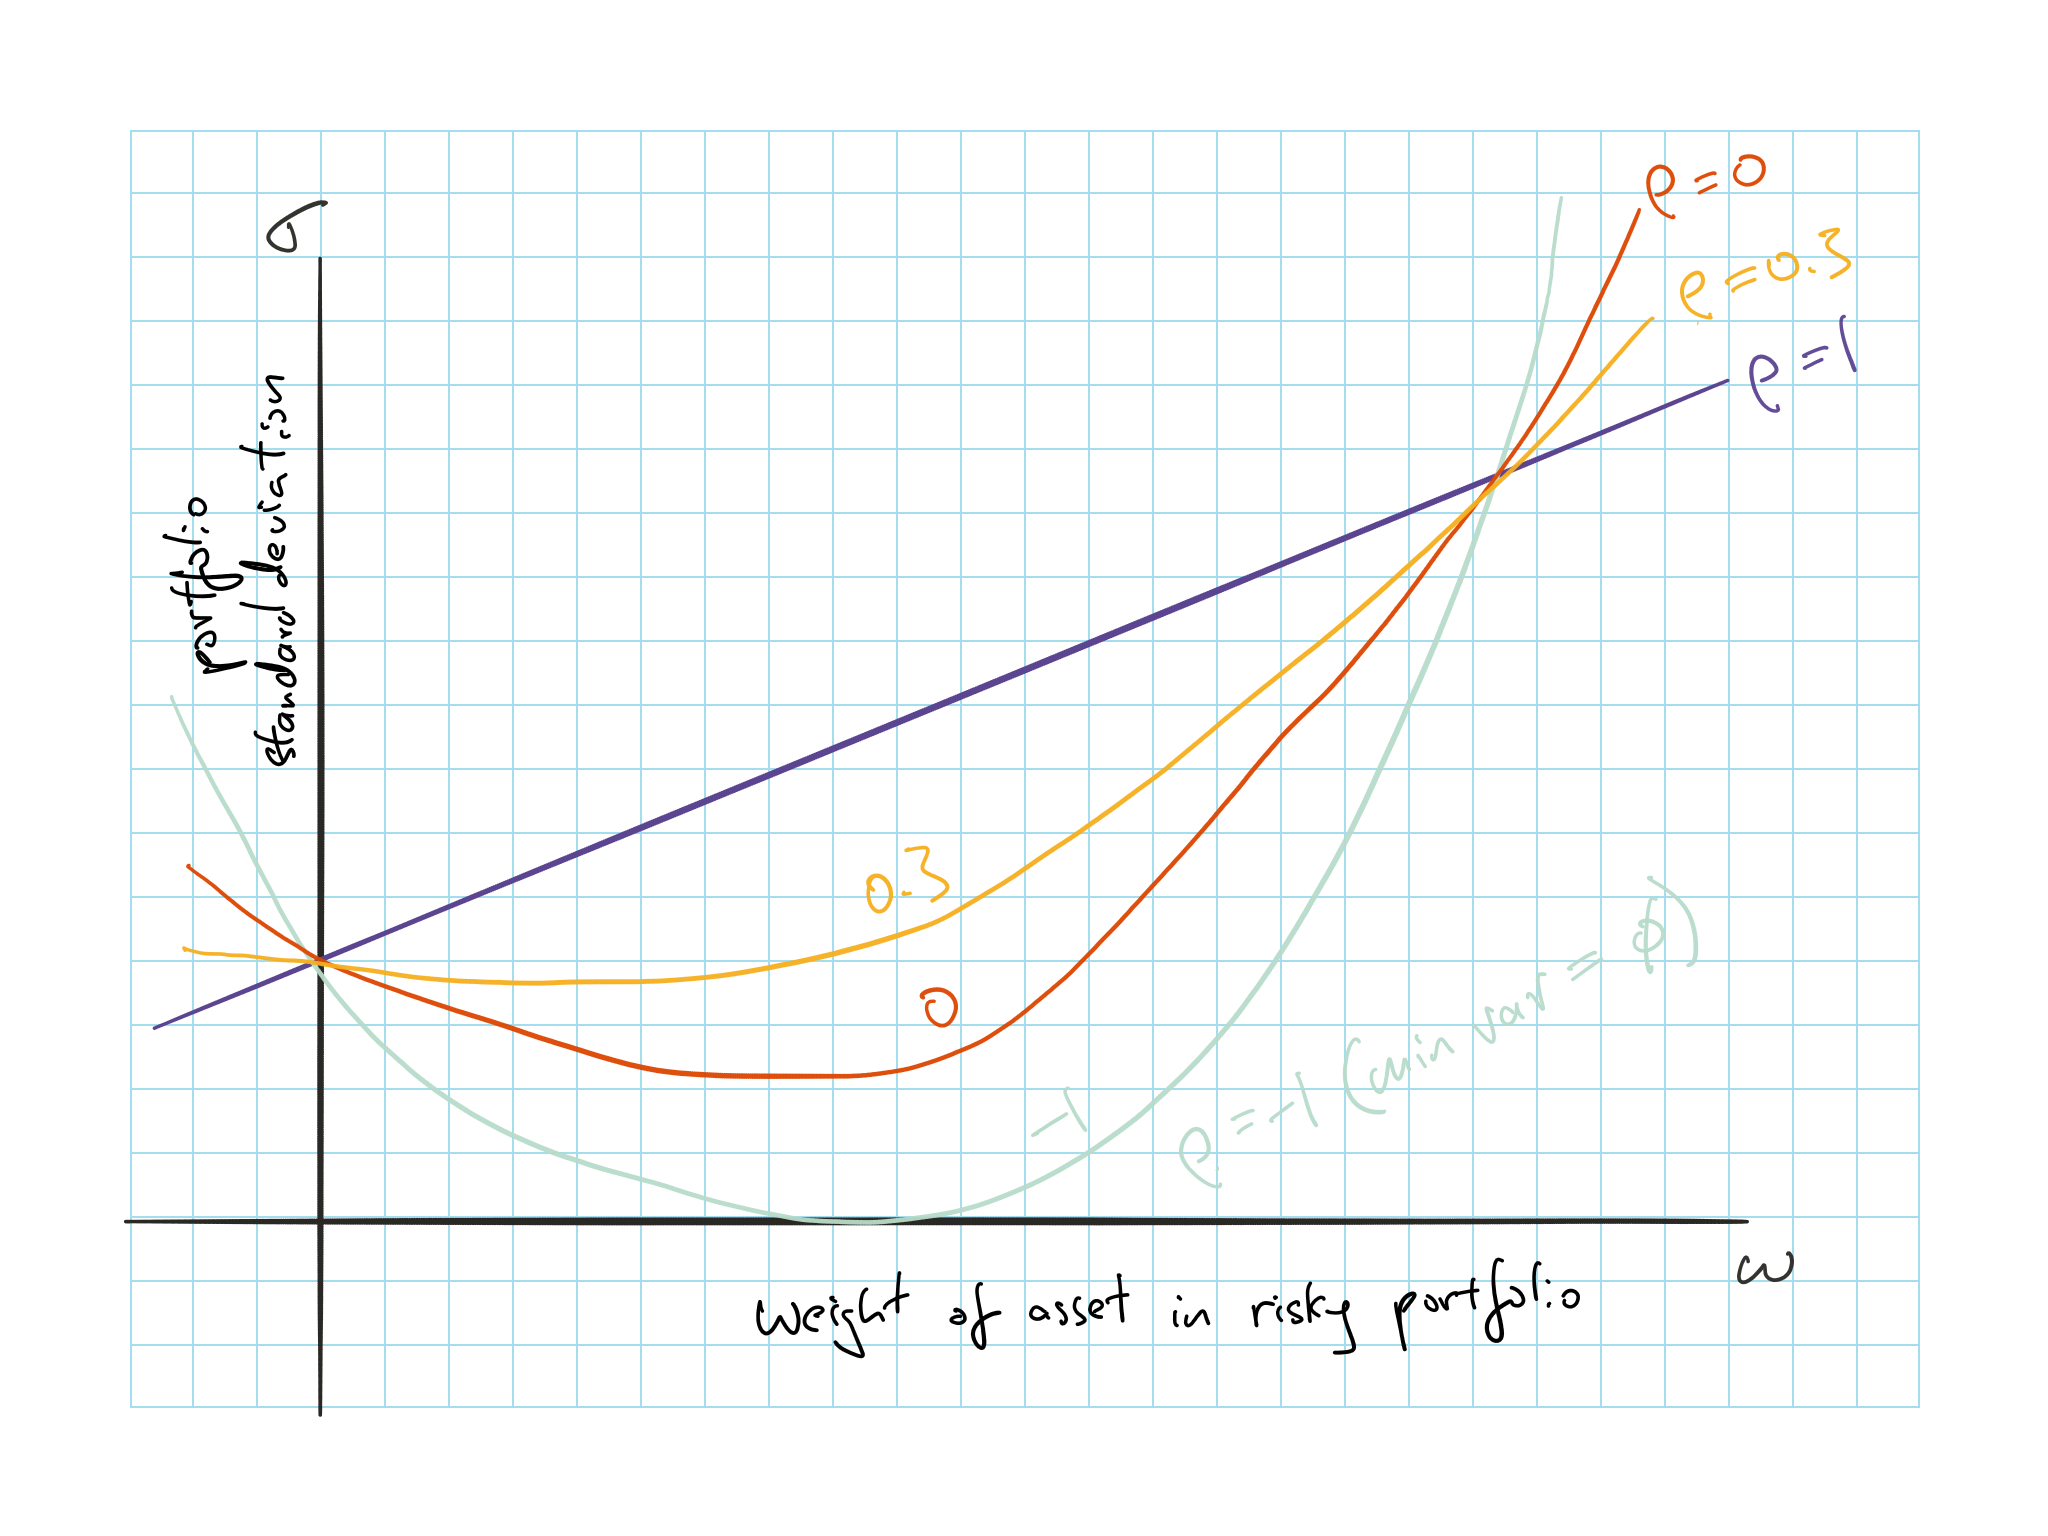
\includegraphics{figures/Exam 9 - 4.png}
\caption{alt text}
\end{figure}

\textbf{Minimum Variance Portfolio}\\
Portfolio with the lowest variance that can be constructed from assets
with a given level of correlation

Weights for the minimum variance portfolio

\(w_D^{Min} = \dfrac{\sigma^2_E - \operatorname{Cov}(r_D, r_E)}{\sigma^2_E + \sigma^2_D - 2\cdot\operatorname{Cov}(r_D, r_E)}\)

\(w_E^{Min} = 1 - w_D^{Min}\)

 \textbf{Portfolio Opportunity Set} for a given \(\rho\)

\begin{figure}[htbp]
\centering
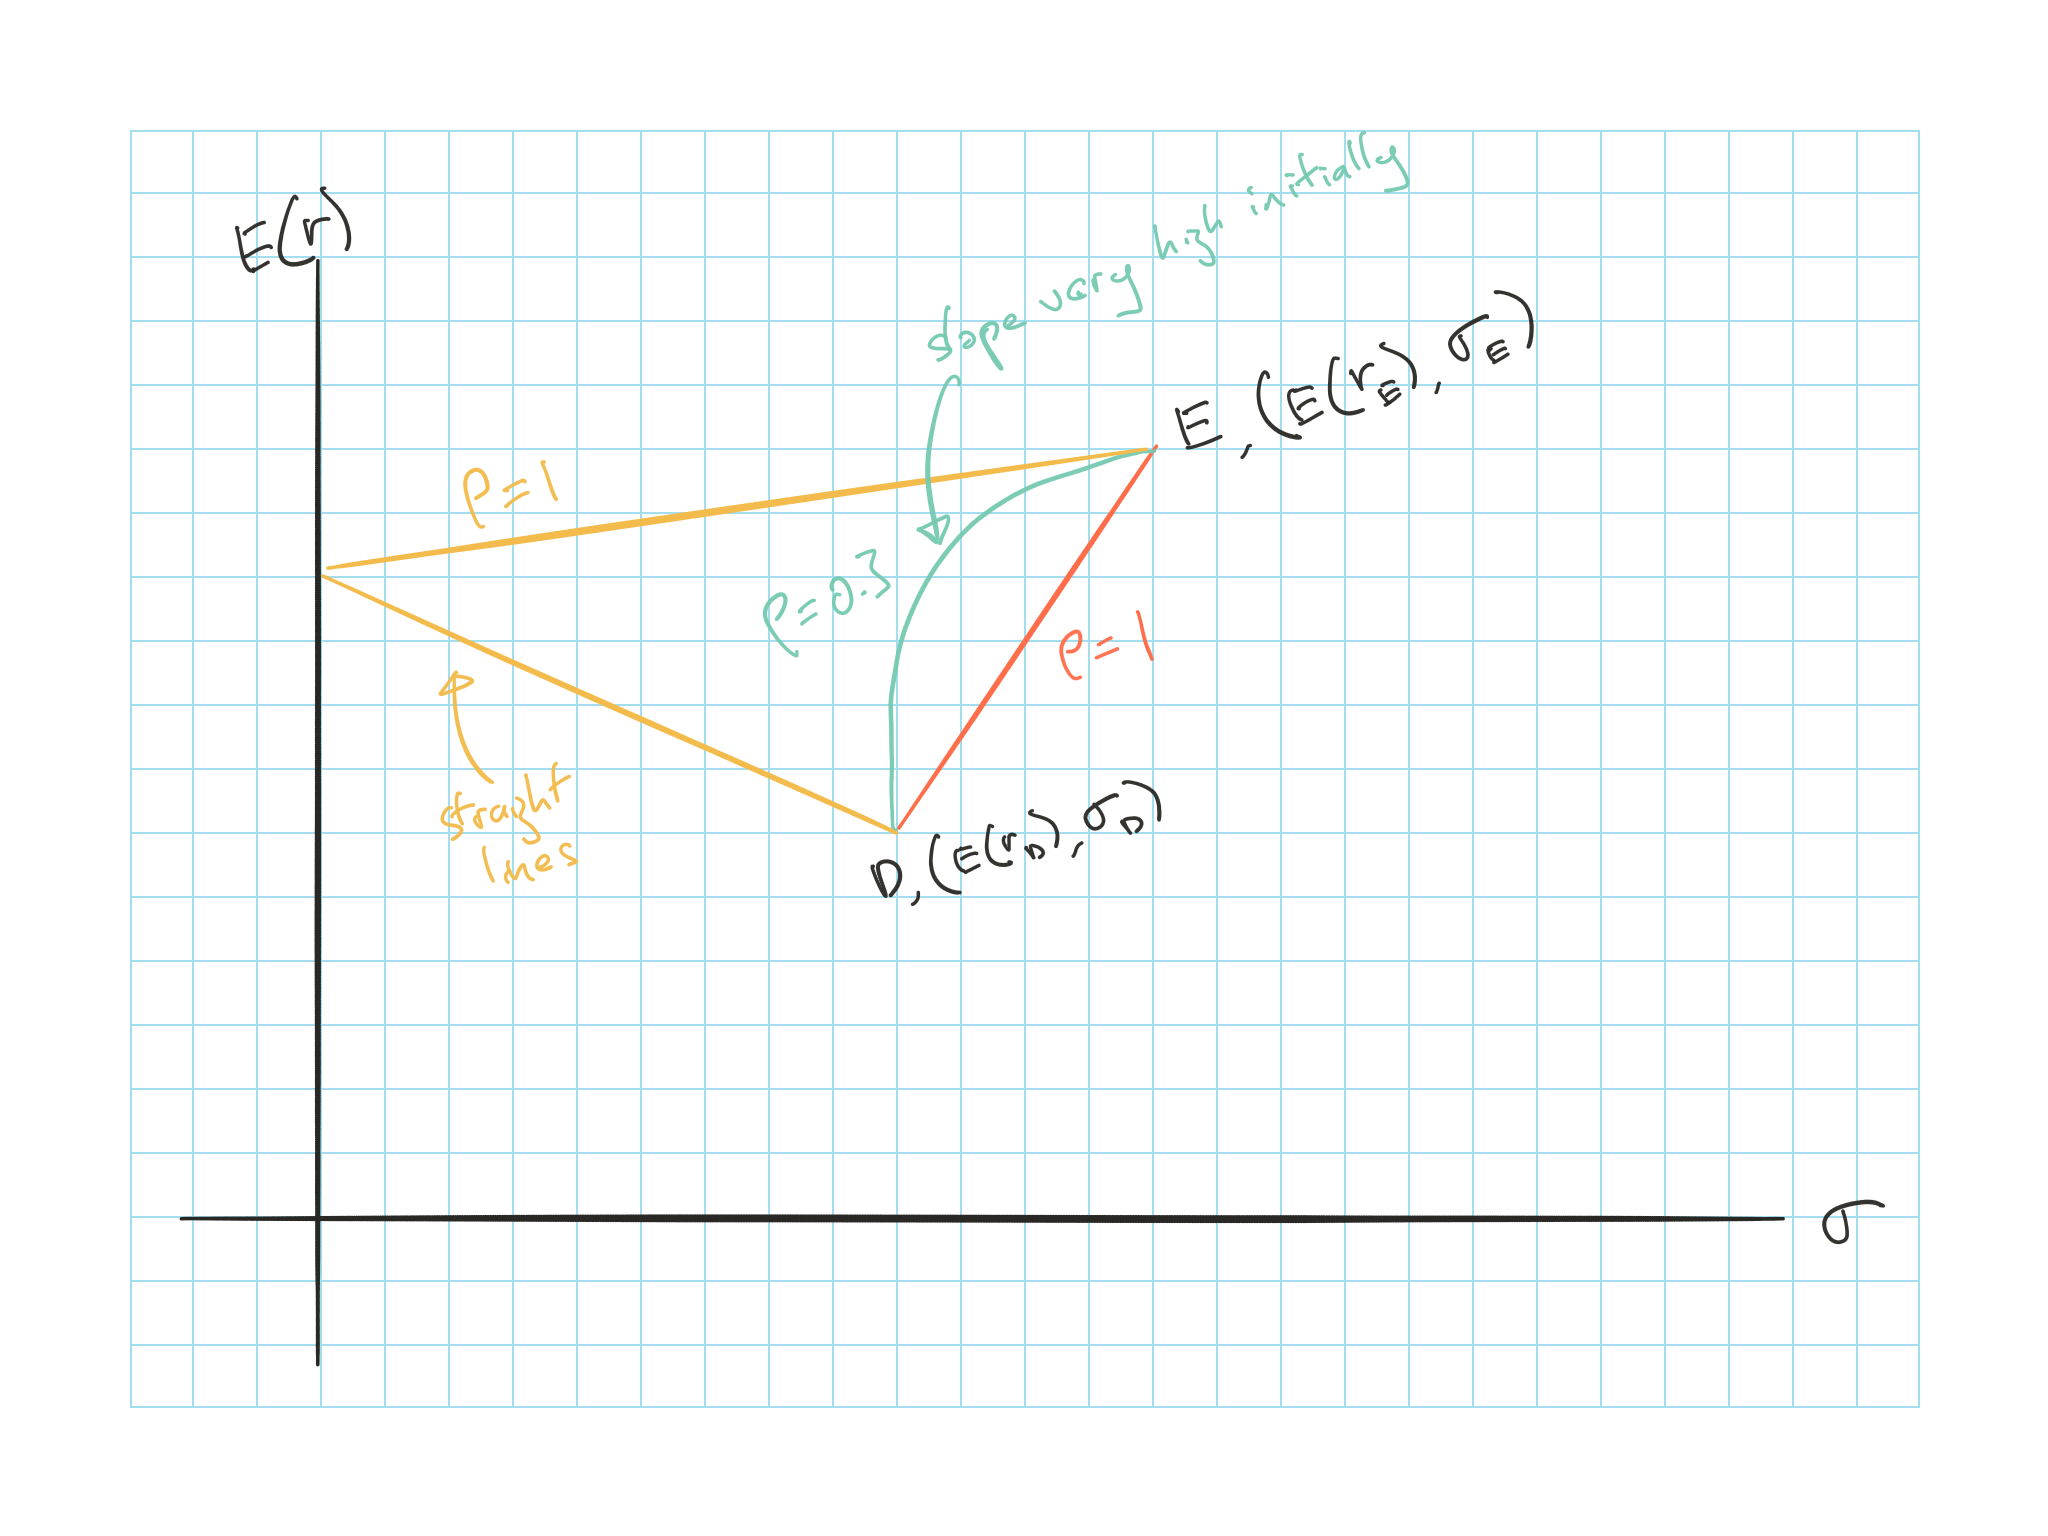
\includegraphics{figures/Exam 9 - 5.png}
\caption{alt text}
\end{figure}

\(\operatorname{E}[r_p]\) vs \(\sigma_p\) with varying weights for a
given \(\rho\)

For assets with \(\rho = -1\) you can achieve \(\sigma = 0\)

For assets perfectly correlated the minimum variance is investing all in
the asset with lower risk

\section{\texorpdfstring{Portfolios of 2 Risky and a \(r_f\)
Assets}{Portfolios of 2 Risky and a r\_f Assets}}\label{portfolios-of-2-risky-and-a-r_f-assets}

\begin{figure}[htbp]
\centering
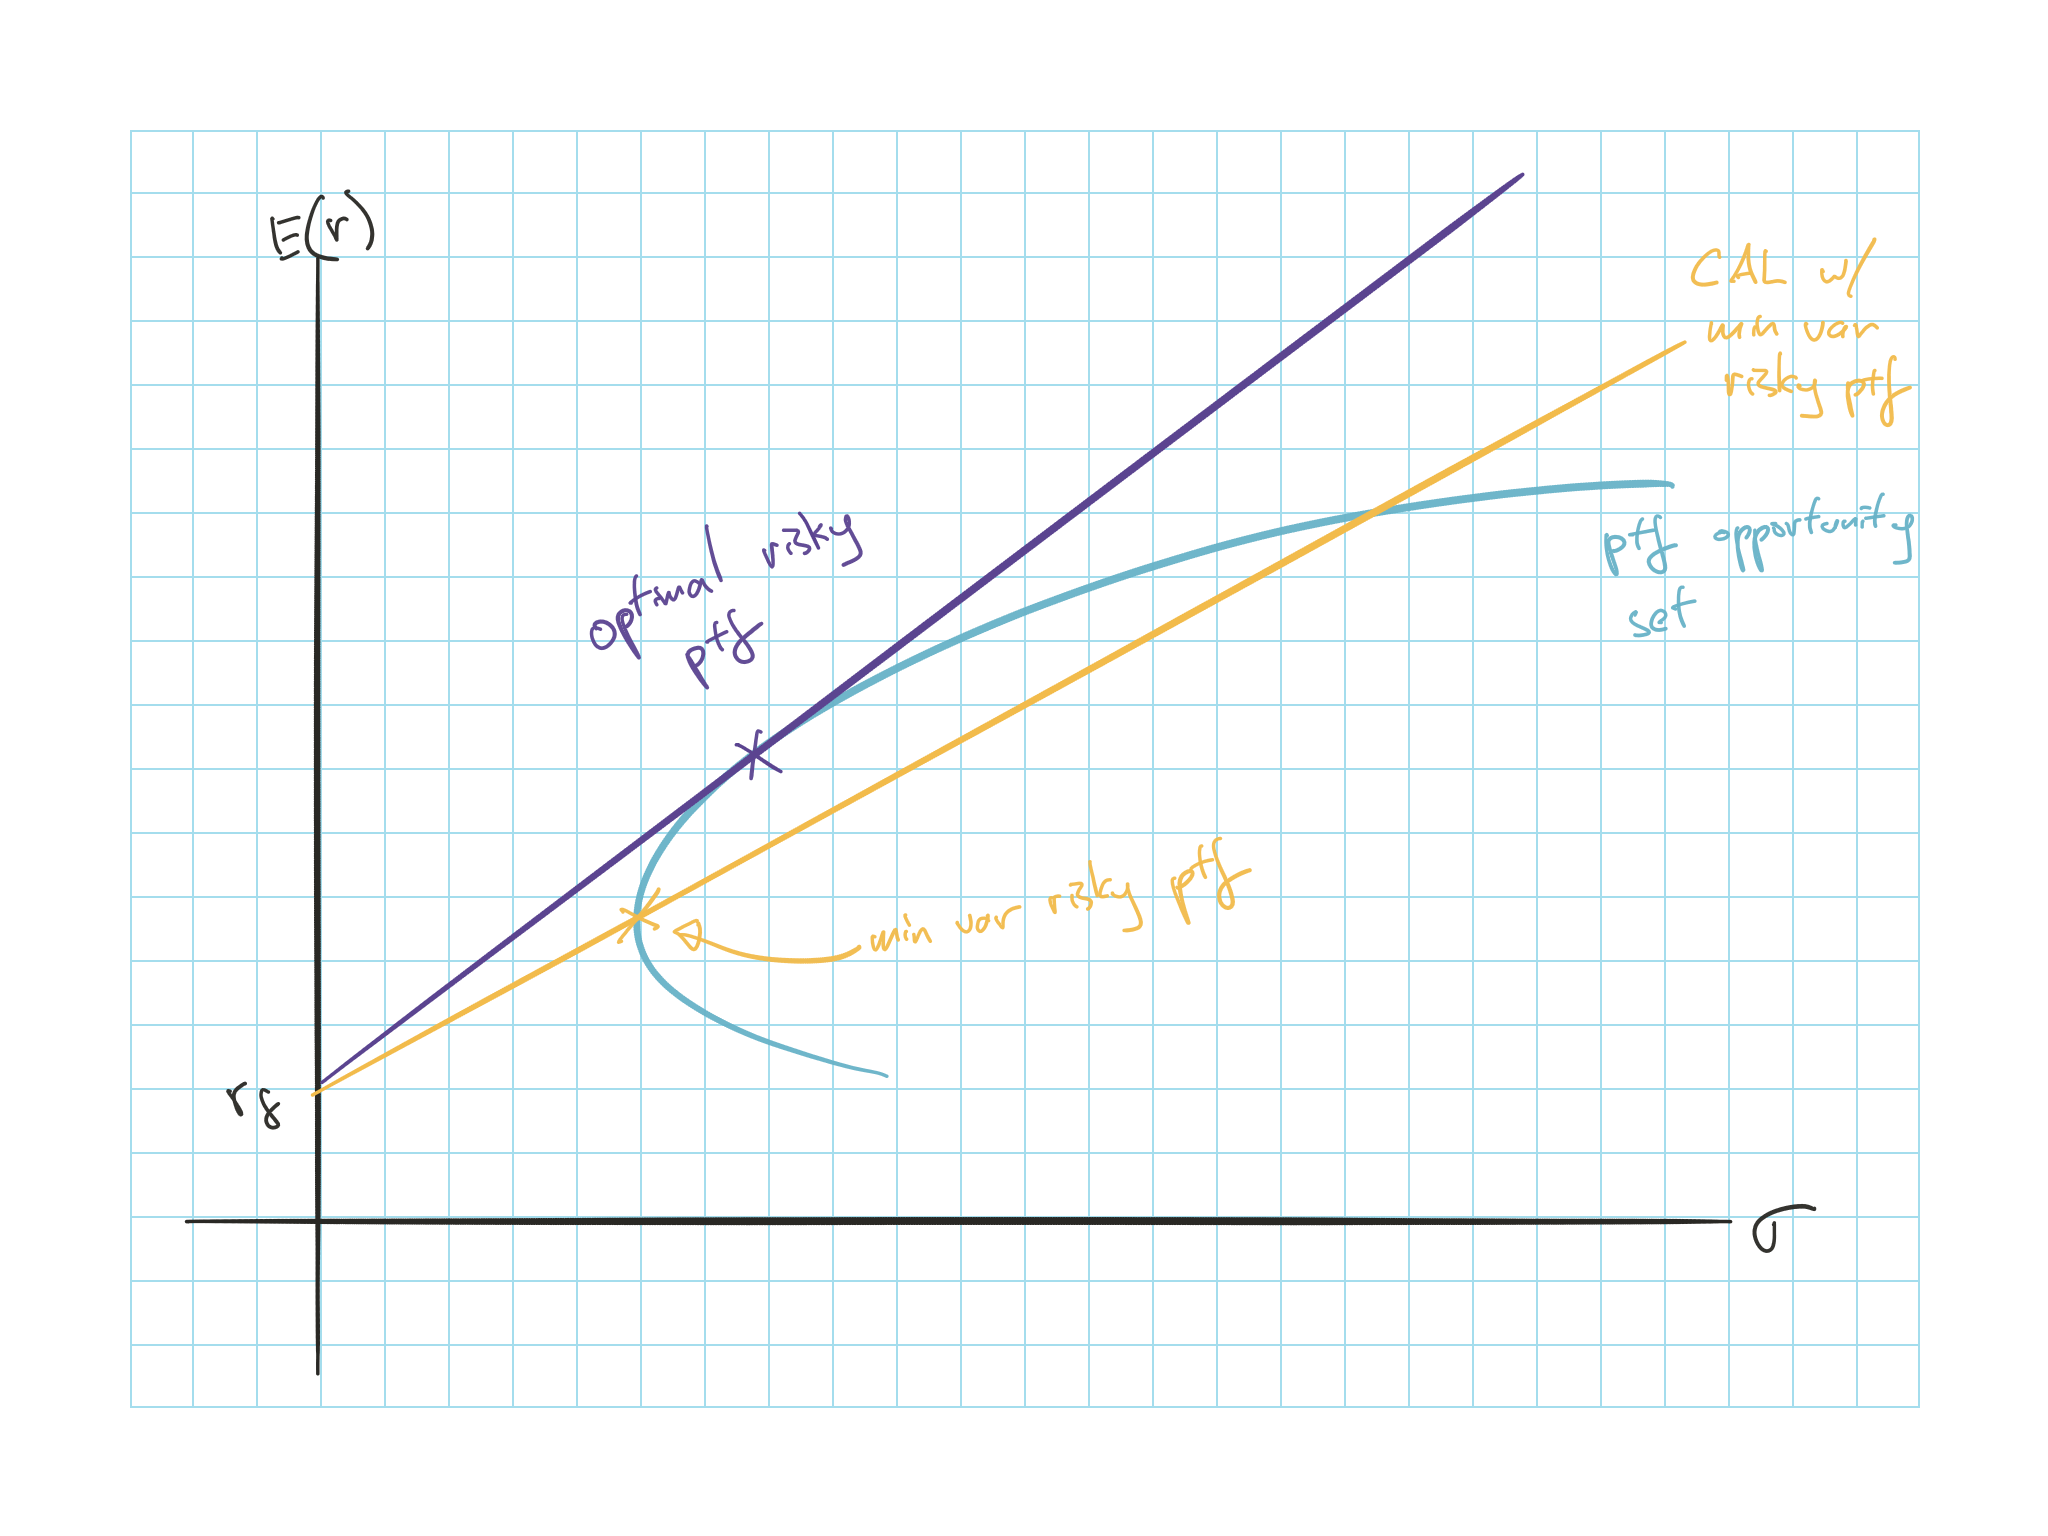
\includegraphics{figures/Exam 9 - 6.png}
\caption{alt text}
\end{figure}

\textbf{Optimal Risky Portfolio}\\
Available portfolio with \textbf{highest Sharpe ratio}

\begin{itemize}
\item
  Portfolio formed where the CAL is tangential to the portfolio
  opportunity set
\item
  This only consist of risky assets, only use the CAL to identify the
  best weight of risky assets (weight between risky portfolio P and
  \(r_f\) is determined later)
\end{itemize}

Minimum variance portfolio is \emph{not} the optimal portfolio

\begin{itemize}
\tightlist
\item
  CAL with minimum variance portfolio does not yield the greatest Sharpe
  ratio
\end{itemize}

Weights of the optimal risky portfolio:

\(w_D = \dfrac{\operatorname{E}[R_D]\sigma^2_E - \operatorname{E}[R_E] \operatorname{Cov}(r_D, r_E)}{\operatorname{E}[R_D]\sigma^2_E + \operatorname{E}[R_E]\sigma^2_D - \left( \operatorname{E}[R_D] + \operatorname{E}[R_E] \right) \operatorname{Cov}(r_D, r_E)}\)

\begin{itemize}
\tightlist
\item
  \(R_D = r_D - r_f\) = XS return over risk free
\end{itemize}

\textbf{Optimal Complete Portfolio}

Weights between \(r_f\) and risky portfolio P depends on investors risk
aversion \(A\) as per BKM 6

\begin{figure}[htbp]
\centering
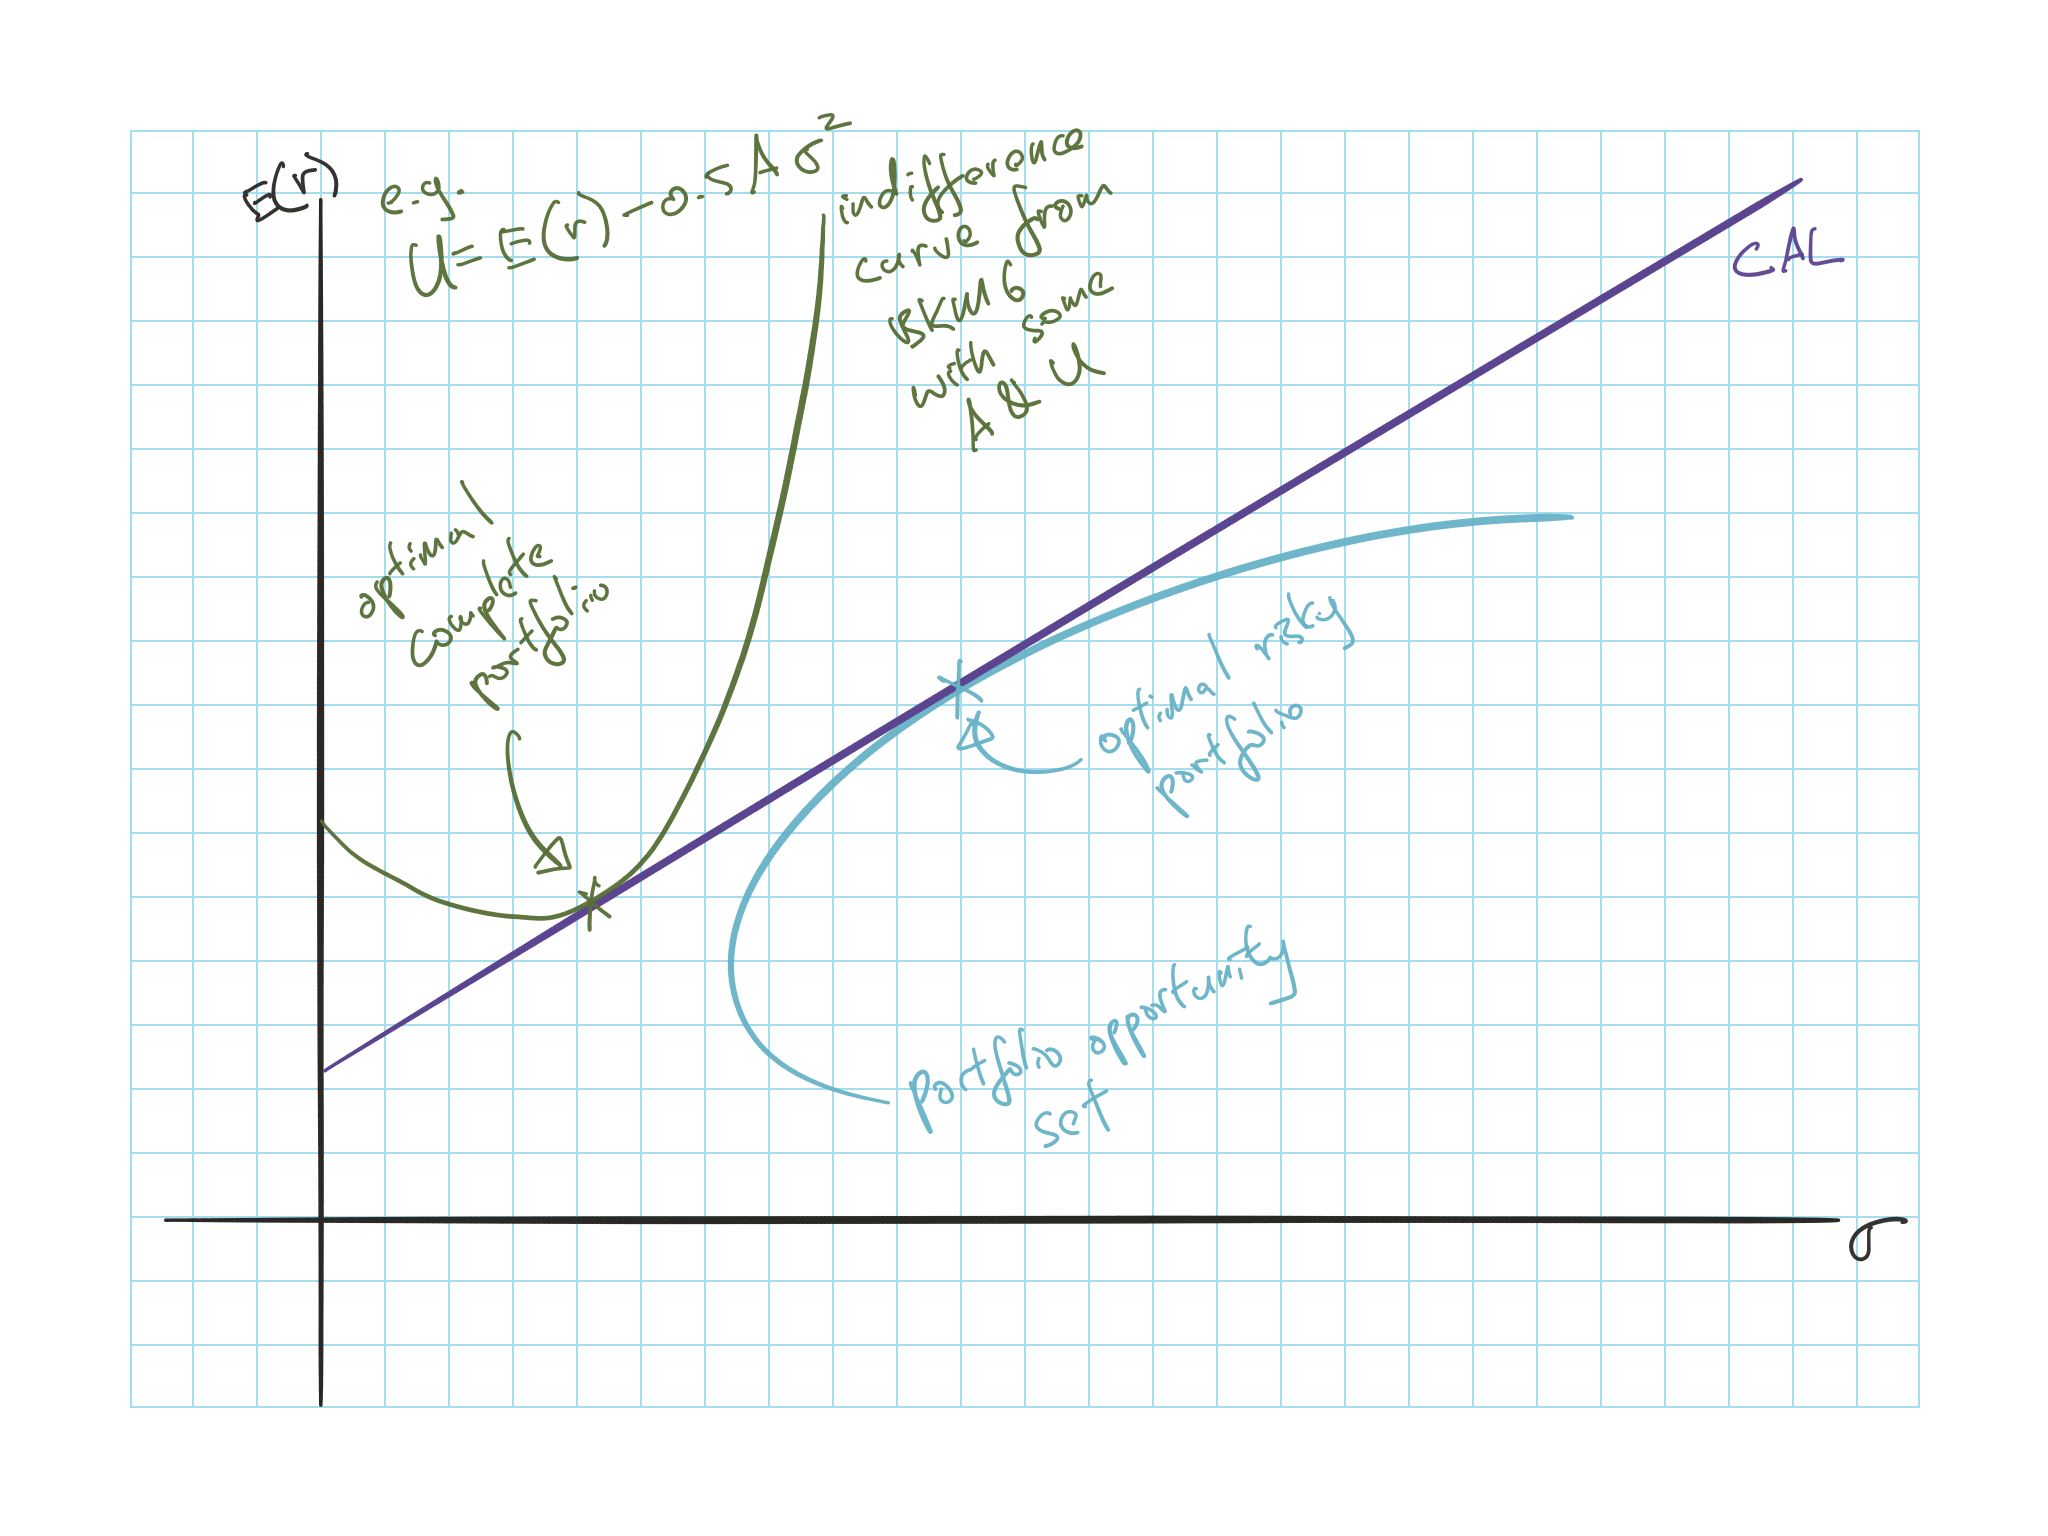
\includegraphics{figures/Exam 9 - 7.png}
\caption{alt text}
\end{figure}

\section{Markowitz Portfolio Selection
Model}\label{markowitz-portfolio-selection-model}

\begin{figure}[htbp]
\centering
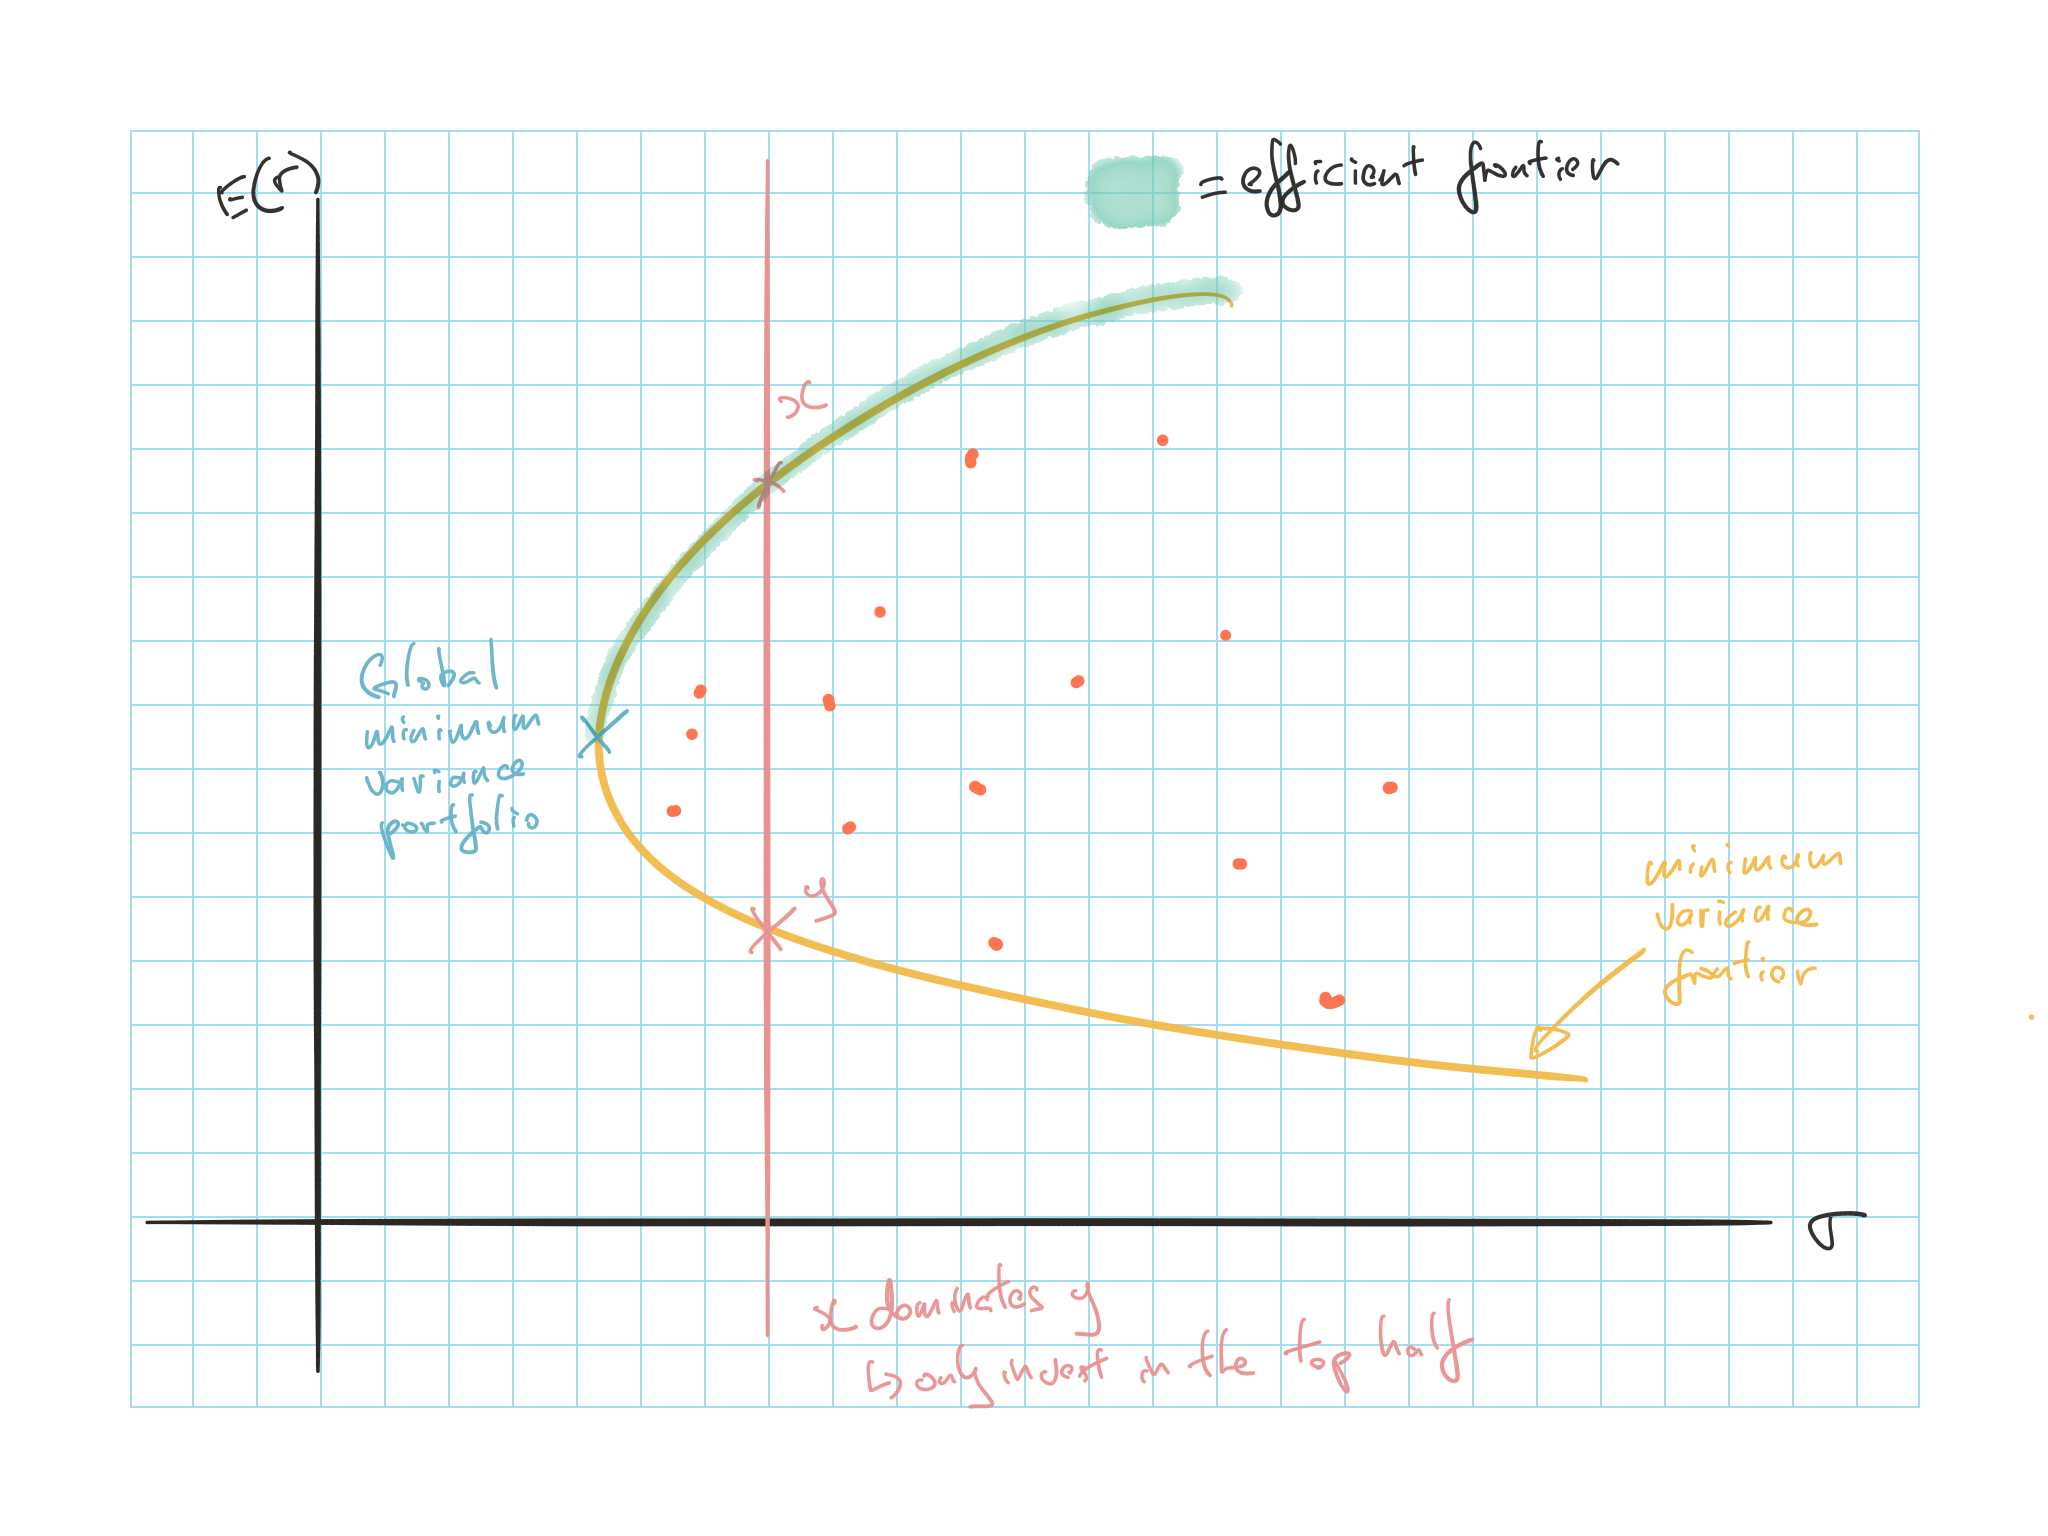
\includegraphics{figures/Exam 9 - 8.png}
\caption{alt text}
\end{figure}

\textbf{Minimum-variance Frontier}\\
Made up of dominant portfolios

\begin{itemize}
\tightlist
\item
  Portfolios with the lowest variance for each level of expected return
\end{itemize}

\textbf{Global Minimum-variance porfolio}\\
Portfolio with the lowest variance

\textbf{Efficient Frontier}\\
Portion of the minimum-variance frontier above the global
minimum-variance portfolio

\textbf{Disadvantages}

\begin{itemize}
\item
  The number of estimates required to run the Markowitz model is
  enormous for many stocks. The expected return and variance estimates
  for each stock needs to be estimated, in addition to the covariances
  between every stock
\item
  Having to make so many estimates, increases the chance of producing
  nonsensical results. In particular, the covariances may not make sense
  when all the data is rolled up
\end{itemize}

\begin{center}\rule{0.5\linewidth}{\linethickness}\end{center}

Expected return and variance of the optimal complete portfolio

\(\operatorname{E}[r_p] = \sum_i w_i \operatorname{E}[r_i]\)

\(\sigma^2_p = \sum_i \sum_j w_i w_j \operatorname{Cov}(r_i, r_j)\)

\section{Separation Principle}\label{separation-principle}

Optimal risky portfolio P is the same for all investors

Difference between investors is the portion of the complete portfolio in
the risky portfolio vs risk free asset driven by investor's risk
aversion \(A\)

2 steps in portfolio selection under \textbf{separation principle}:

\begin{enumerate}
\def\labelenumi{\arabic{enumi})}
\item
  Select optimal risky portfolio

  \begin{itemize}
  \item
    This only differs depending on the analyst
  \item
    CAL is the same for all investors
  \end{itemize}
\item
  Select the optimal complete portfolio

  \begin{itemize}
  \item
    Allocate between risk free vs risky assets depending on investors
    \(A\)
  \item
    Investor's \(A\) dictates where the optimal complete portfolio lies
    on the CAL
  \end{itemize}
\end{enumerate}

\section{Asset Allocation vs Security
Selection}\label{asset-allocation-vs-security-selection}

So far focused has been on \emph{asset allocation}

\begin{itemize}
\tightlist
\item
  Allocation of a complete portfolio to the various asset categories
\end{itemize}

Step 1: Asset allocation

\begin{itemize}
\tightlist
\item
  Figure out how much to allocate to each asset class
\end{itemize}

Step 2: Security selection

\begin{itemize}
\tightlist
\item
  Select specific securities in order to try increase return
\end{itemize}

Procedure of optimal security selection is the same as the procedure of
optimal asset allocation in the above sections

Since it's impossible to be expert in all securities from all asset
class, after allocating money to the different asset classes, consult
expert for the security selection in each class

\section{Risk Pooling vs Risk
Sharing}\label{risk-pooling-vs-risk-sharing}

\subsection{Risk Pooling}\label{risk-pooling}

\textbf{Risk pooling} involves merging several uncorrelated projects
together, aka the \textbf{insurance principle}

\begin{itemize}
\item
  Does not reduce risk (sharpe ratio and \(\sigma\) both increase)
\item
  Increases the total exposure to risk
\item
  As investor increase the risk pooling to include \(n\) assets, both
  the Sharpe ratio and \(\sigma\) will increase by \(n^{0.5}\) for asset
  with the same \(R\) and \(\sigma\) that is uncorrelated with each
  other
\end{itemize}

\subsection{Risk Sharing}\label{risk-sharing}

\textbf{Risk sharing} involves taking a fixed amount of risk and sharing
it among several investors

\begin{itemize}
\item
  Selling shares of an risky portfolio so that total investment remains
  constant
\item
  Increase Sharpe ratio and reduce total risk
\end{itemize}

Practical perspective:

\begin{itemize}
\item
  Reduce risk by selling share of the insurer to investors
\item
  Assuming that the total risk per investor remains constant, Sharpe
  ratio will increase as the \# of policies written increases
\end{itemize}

Caveat:

\begin{itemize}
\item
  Disadvantages of managing a very large firm and will put pressure on
  the profit margin
\item
  Impact of any error when estimating the risk of the insured will be
  compounded over many policies
\end{itemize}

\section{Investment for the Long Run}\label{investment-for-the-long-run}

\textbf{Time diversification} is not true and does not reduce risk

\begin{itemize}
\item
  Volatility of the \emph{average} annual return do go down, but
\item
  Volability of the dollar return increase with the time
\item
  Extending investment horizon for an additional period is similar to
  adding additional risky asset
\item
  Similar to risk pooling
\item
  To increase Sharpe ratio while maintaining the same level of risk,
  investor needs to half the investment if double the time horizon
\end{itemize}

\section{Past Exam Questions}\label{past-exam-questions-1}

 2003, Q5 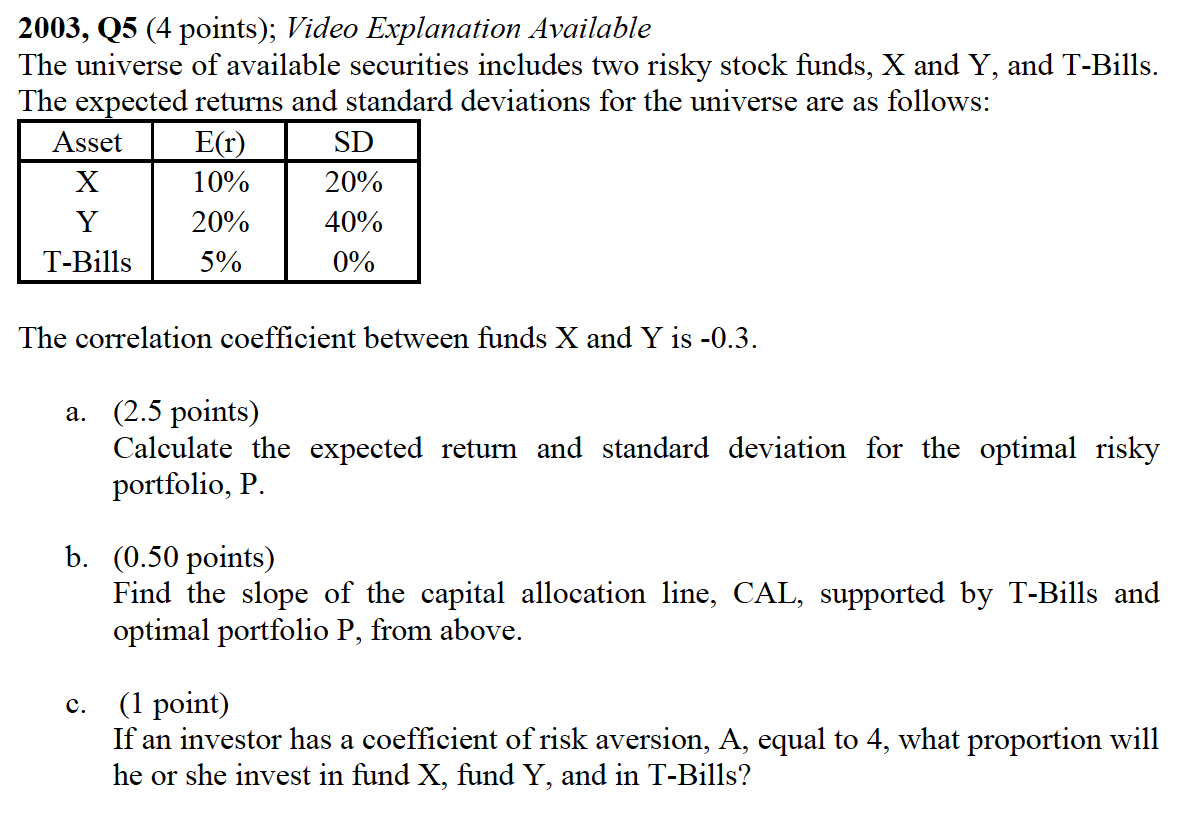
\includegraphics{questions/2003-5Q.png}
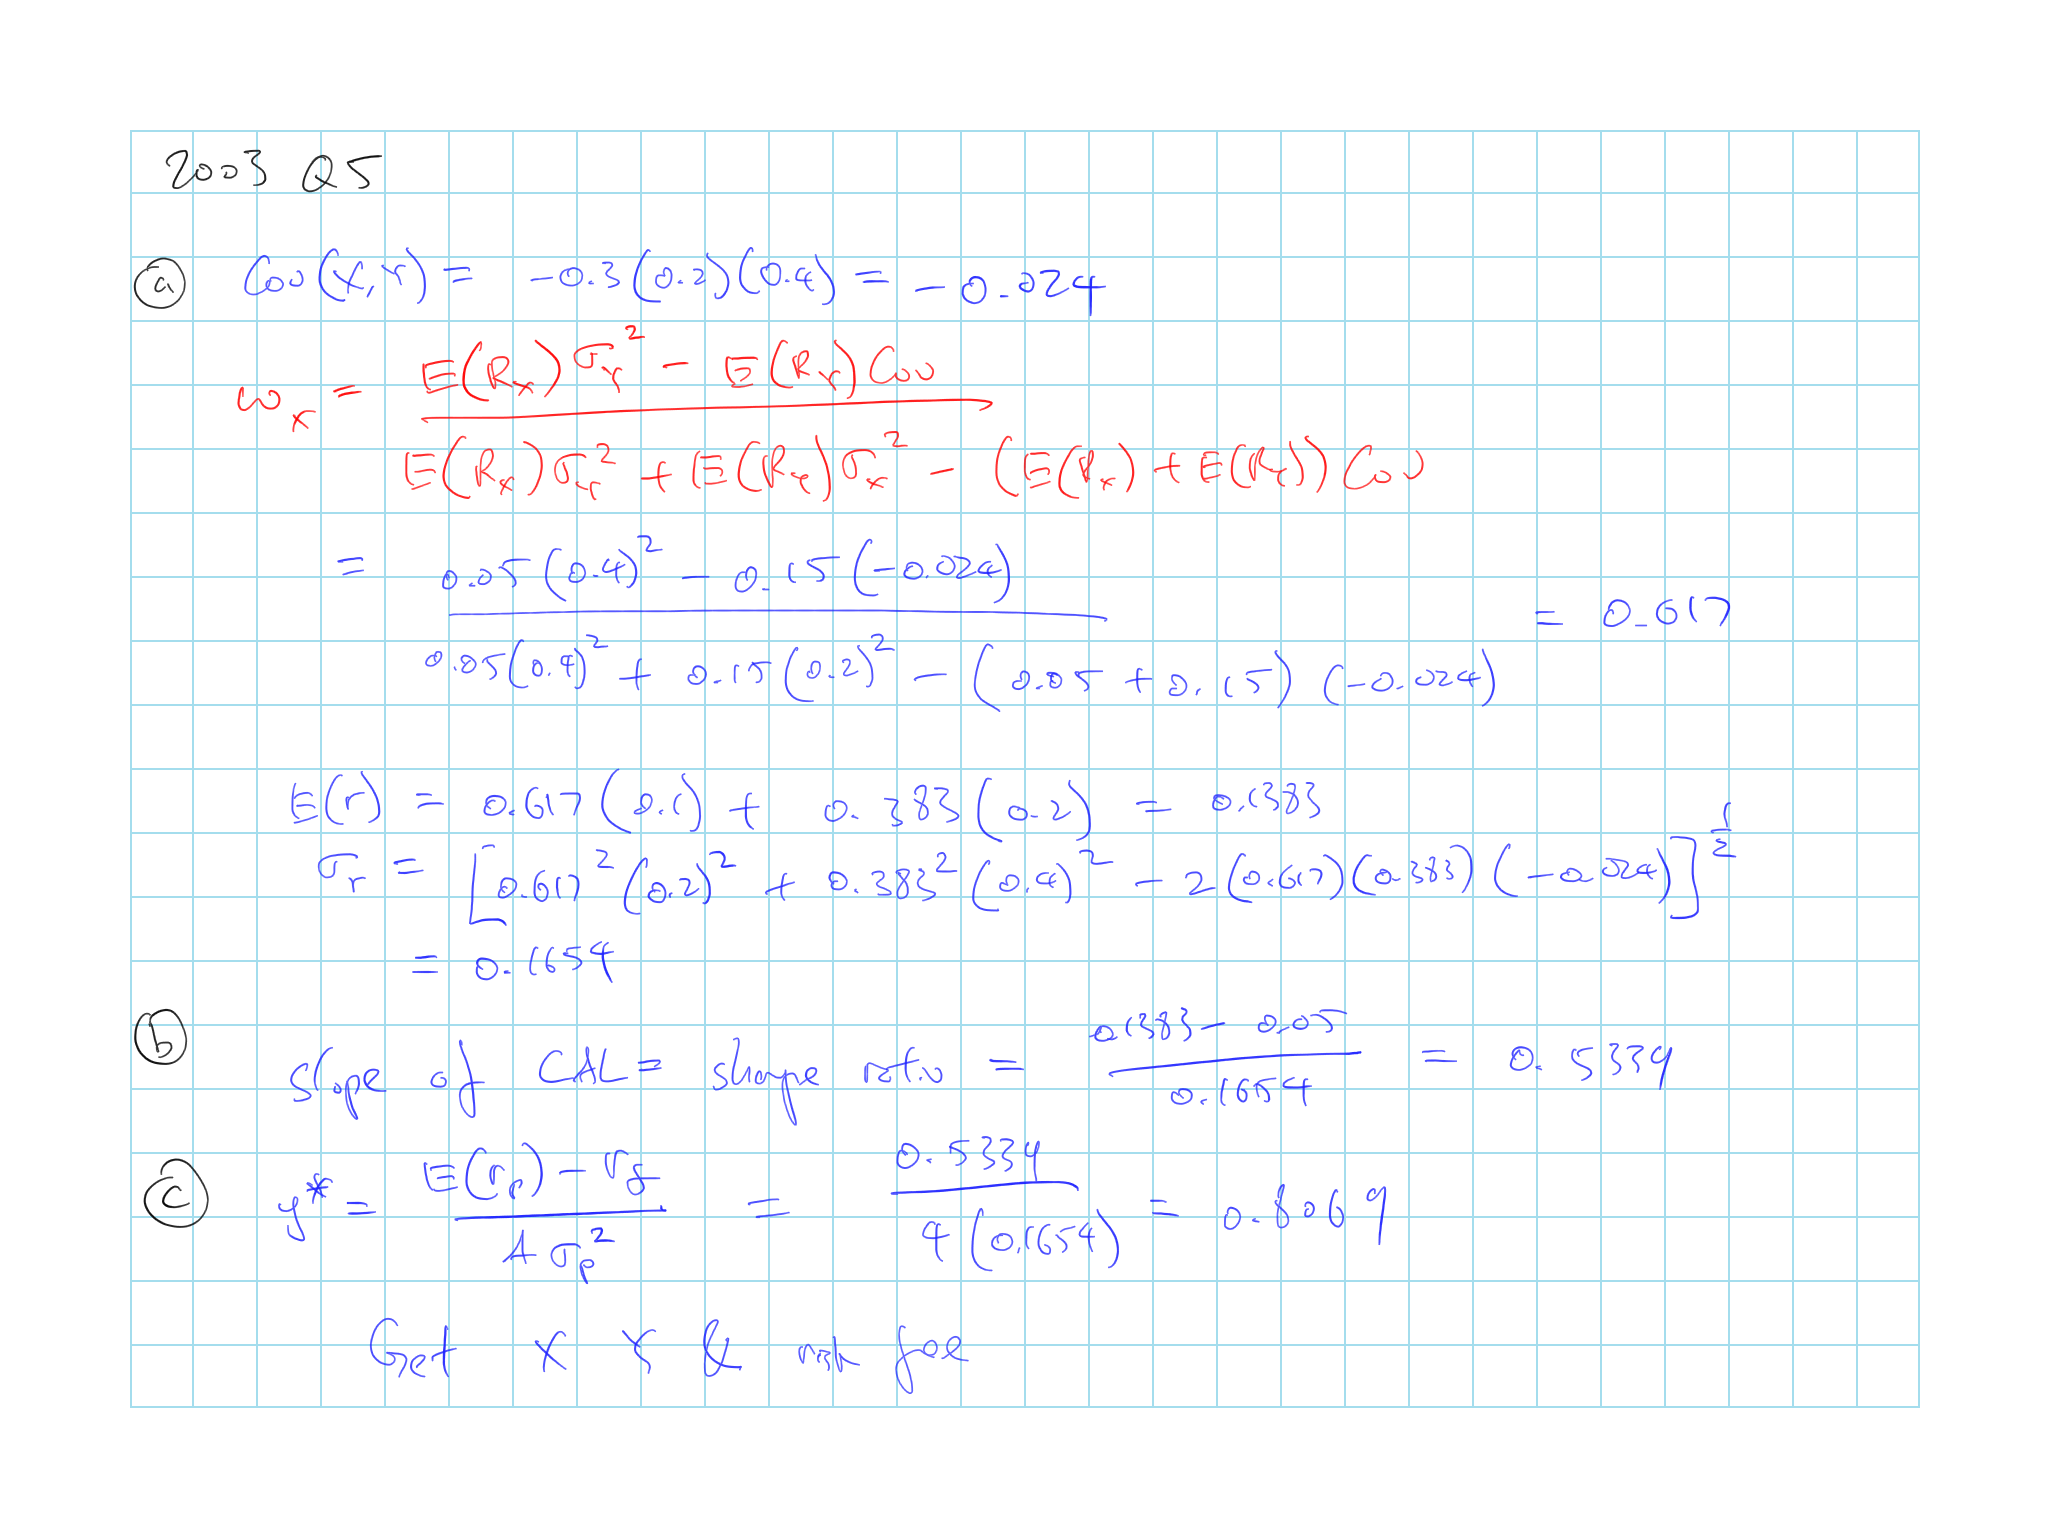
\includegraphics{questions/2003-5A.png}

 2009, Q3 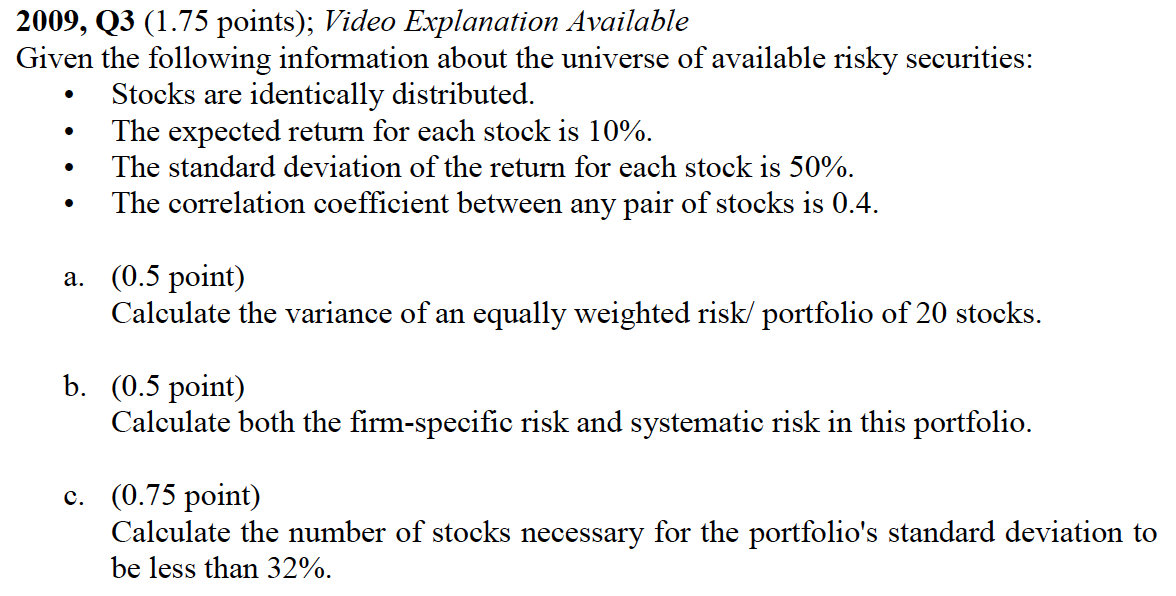
\includegraphics{questions/2009-3Q.png}
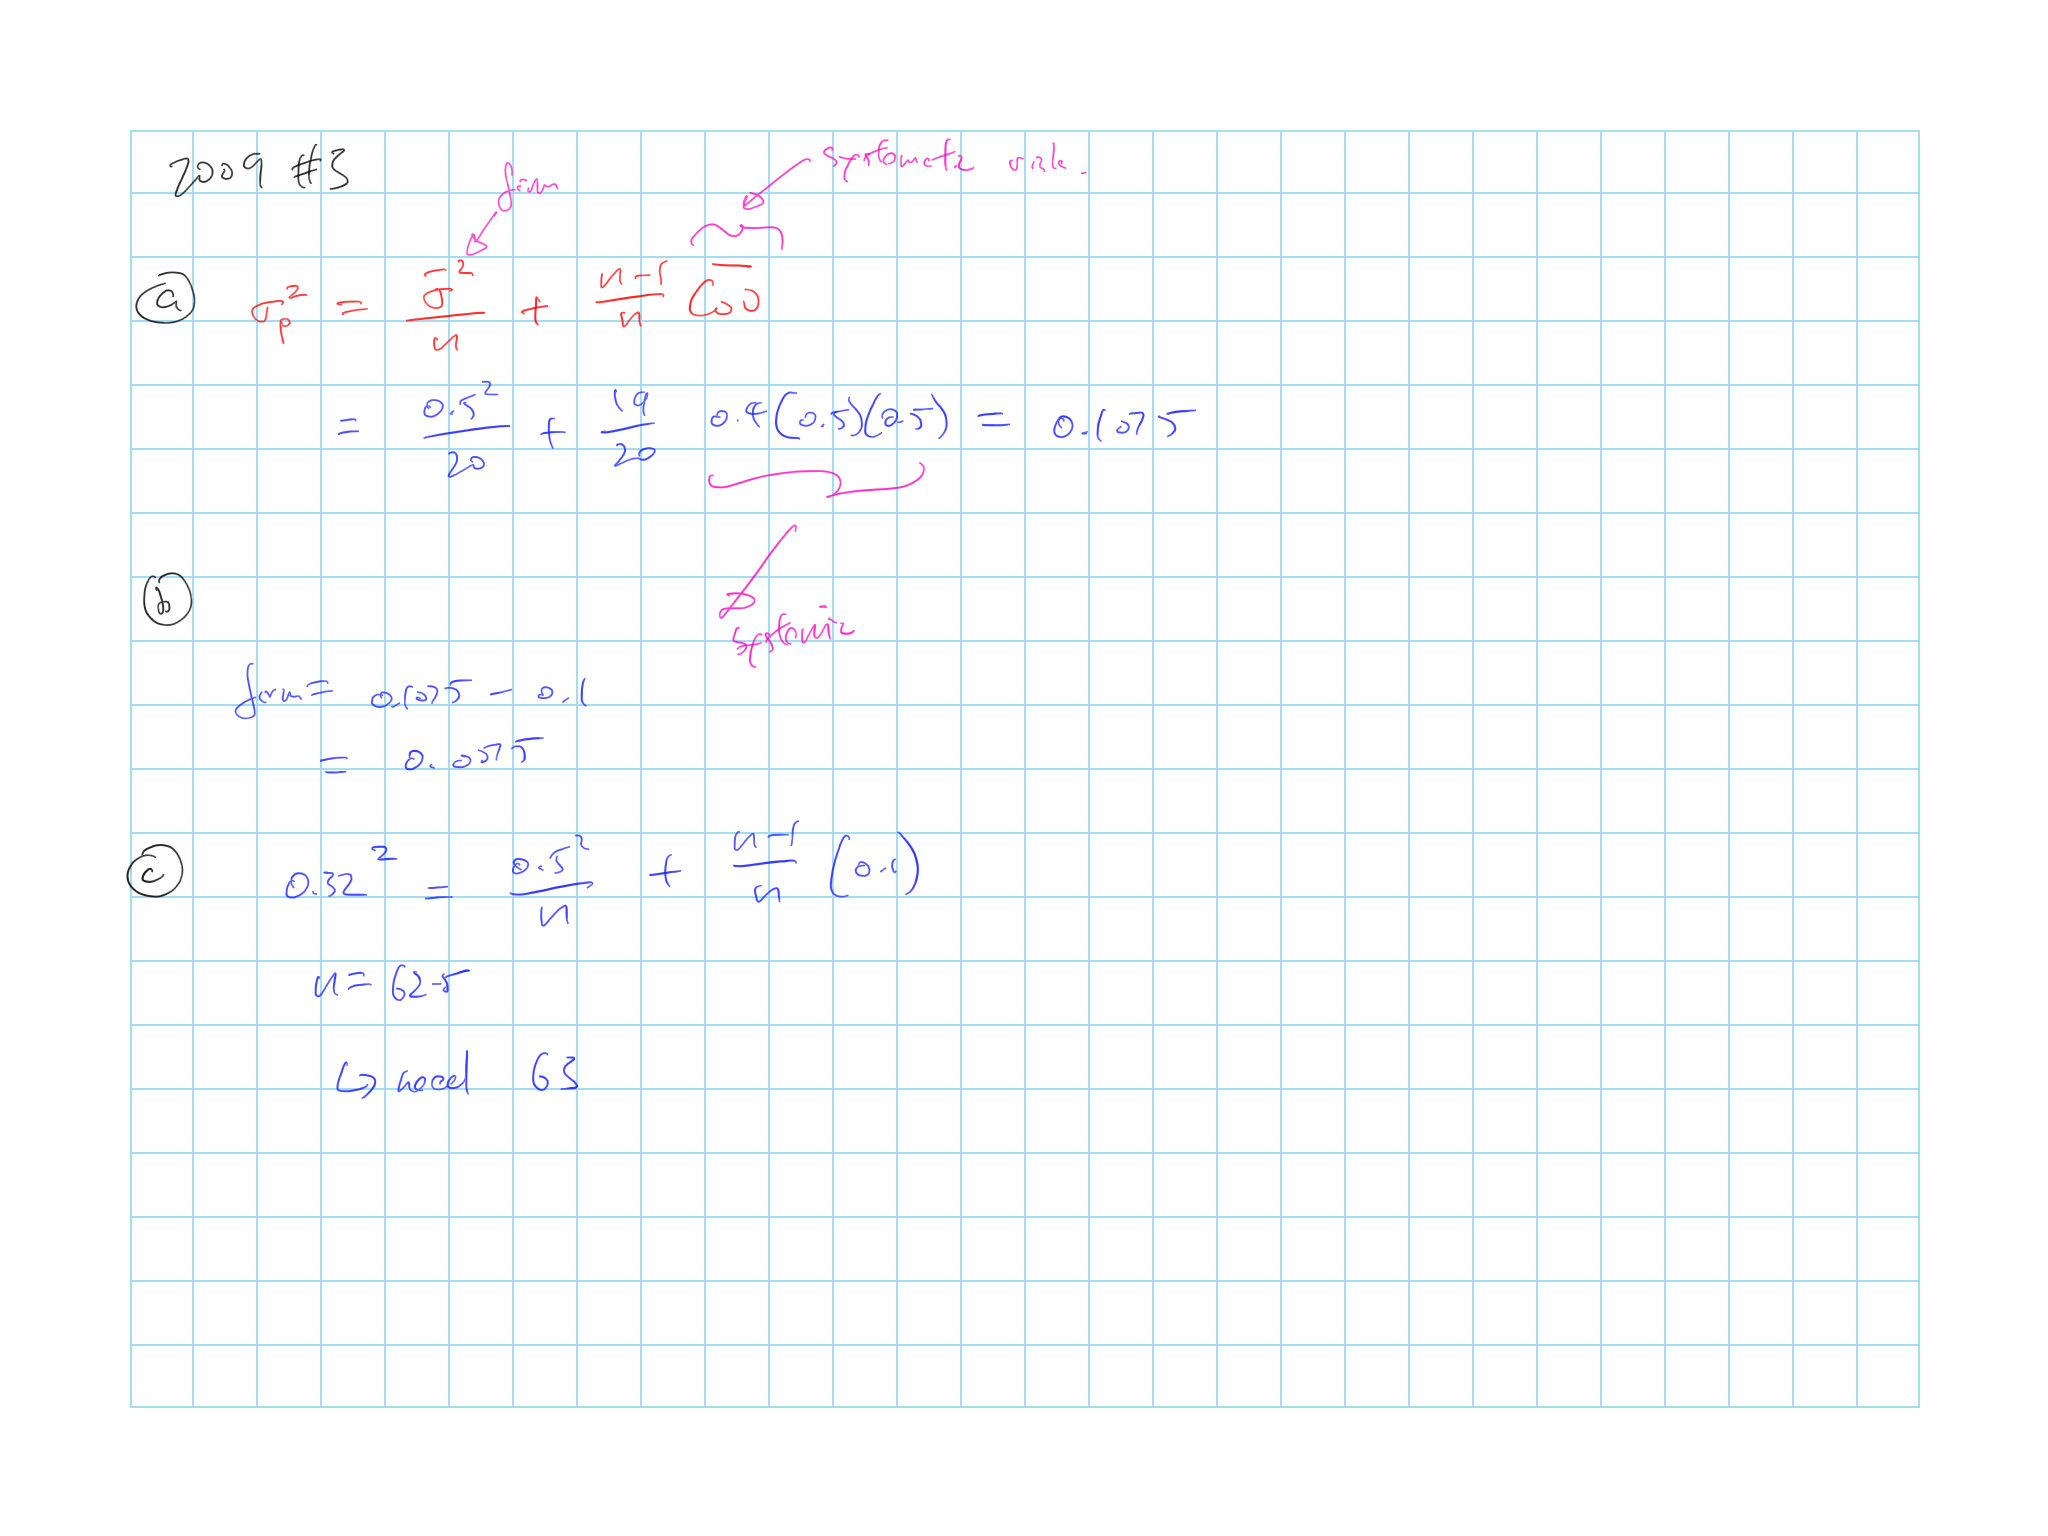
\includegraphics{questions/2009-3A.png}

 2015, Q1 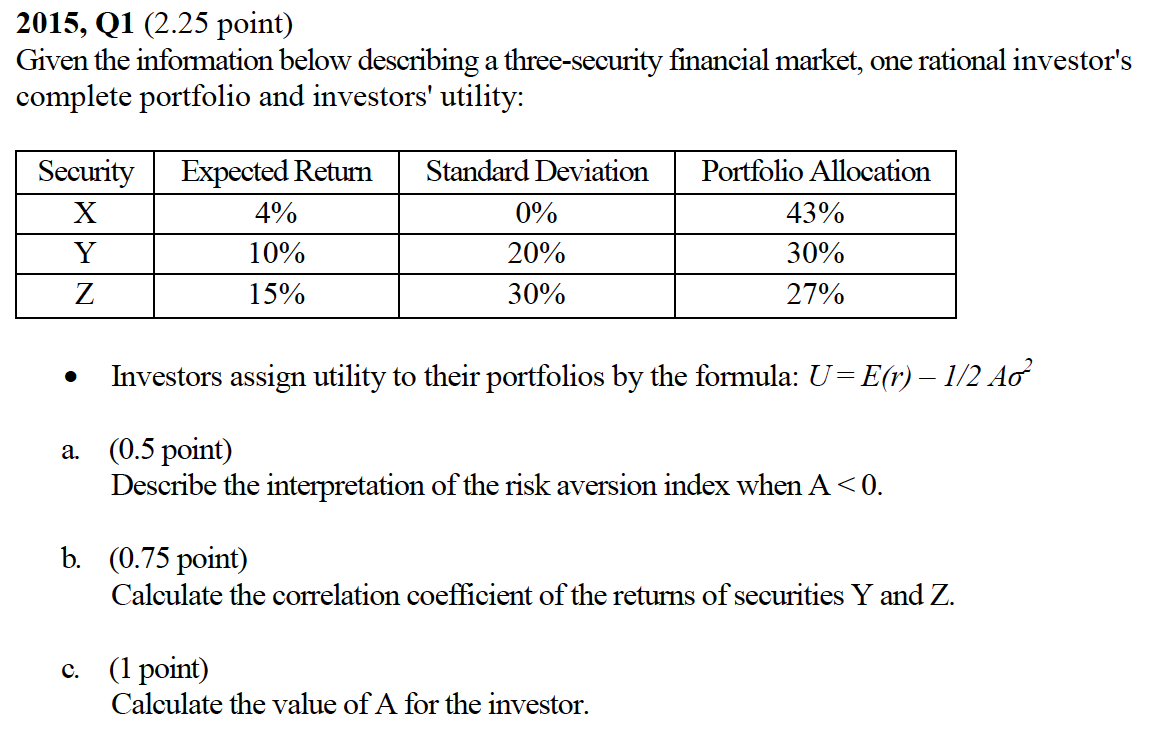
\includegraphics{questions/2015-1Q.png}
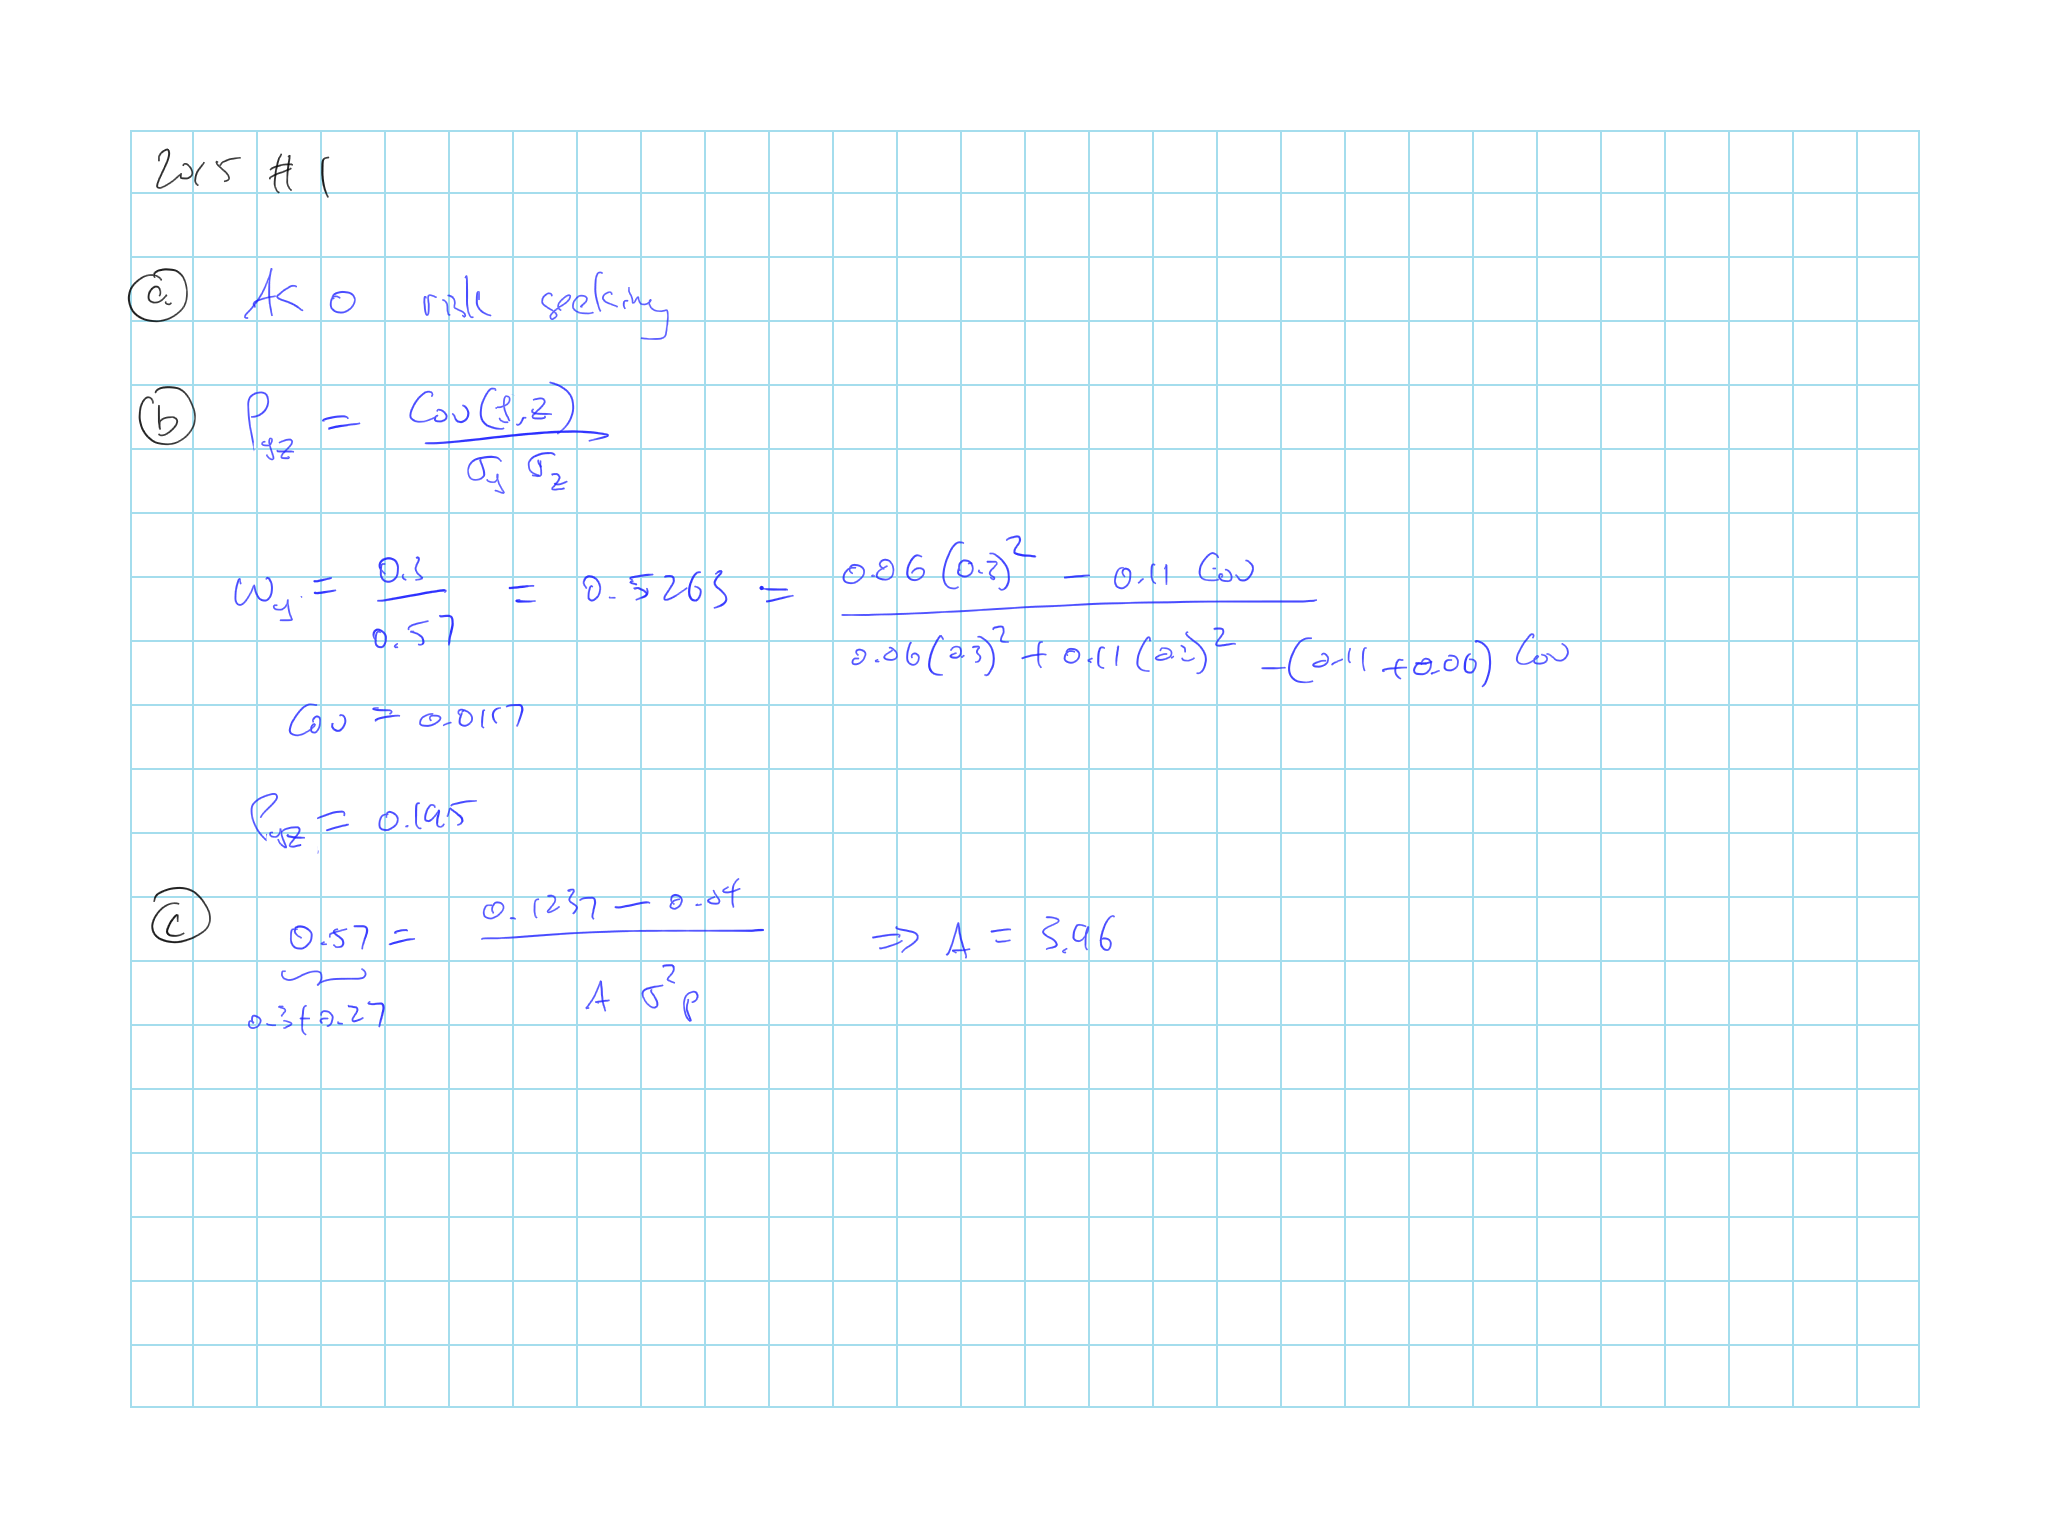
\includegraphics{questions/2015-1A.png}

\chapter{A3 BKM8: Index Models}\label{a3-bkm8-index-models}

Z. Bodie, A. Kane, A. Marcus

\section{Cliff's Summary}\label{cliffs-summary-2}

\protect\hyperlink{single-factor}{\textbf{Single Factor Model}}

\(r_i = \operatorname{E}[r_i] + \beta_i m + e_i\)

\begin{itemize}
\tightlist
\item
  Assumptions and source of uncertainty
\end{itemize}

Variance and covariance

\begin{itemize}
\item
  \(\sigma^2_i = \beta^2_i \sigma^2_m + \sigma^2(e_i)\)
\item
  \(\operatorname{Cov}(r_i, r_j) = \operatorname{Cov}(\beta_i m + e_i, \beta_j m + e_j) = \beta_i \beta_j \sigma^2_m\)
\end{itemize}

\textbf{Single Index Model}

Return Premium with market index \(M\):

\begin{itemize}
\tightlist
\item
  \(R_i(t) = \alpha_i + \beta_i R_M(t) + e_i(t)\)
\end{itemize}

Expected Return Premium:

\begin{itemize}
\tightlist
\item
  \(\operatorname{E}[R_i] = \overbrace{\underbrace{\alpha_i}_{\text{Non-mkt premium}} + \underbrace{\beta_i \operatorname{E}[R_M]}_{\text{Systematic risk premium}}}^{\text{Components of risk premium}}\)
\end{itemize}

\protect\hyperlink{single-index-pros-cons}{Pros and cons} of single
index model

\protect\hyperlink{firm-spec-risk}{Portfolio variance} as number of
stock change

\begin{itemize}
\item
  \(\sigma^2_p = \underbrace{\beta^2_p \sigma^2_m}_{\text{System}} + \underbrace{\sigma^2(e_p)}_{\text{Firm}}\)
\item
  \(\sigma^2(e_p) = \dfrac{\bar{\sigma}^2(e)}{n}\)
\end{itemize}

Security characteristic line

\begin{itemize}
\tightlist
\item
  And other things to do with parameters \(\alpha\) and \(\beta\)
\end{itemize}

\protect\hyperlink{alpha}{Alpha transport}

\protect\hyperlink{ptf-construct}{Portfolio construction}

\begin{enumerate}
\def\labelenumi{\arabic{enumi}.}
\item
  Get the weight between active portfolio based on
  \(\dfrac{\alpha_i}{\sigma^2(e_i)}\) then scale it to 1
\item
  Get the weighted parameters (\(\alpha, \sigma^2(e_i), \beta_i\))
\item
  Use the 2 part formula to get the weight of the active portfolio
  within the total risky portfolio

  \begin{itemize}
  \item
    \(w^*_A = \dfrac{w^0_A}{1 + (1-\beta_A)w^0_A}\)
  \item
    \(w^0_A = \dfrac{ \alpha_A / \sigma^2(e_A)}{\operatorname{E}[R_M] / \sigma^2_m}\)
  \end{itemize}
\item
  Get the weight of the market and weight of the individual stocks
  withint the total risky portfolio (simple math)
\item
  Risk premium and variance of the risky portfolio

  \begin{itemize}
  \item
    \(\operatorname{E}[R_p] = (w^*_M + w^*_A \beta_A) \operatorname{E}[R_M] + w^*_A \alpha_A\)
  \item
    \(\sigma^2_p = (w^*_M + w^*_A \beta_A)^2 \sigma^2_M + \underbrace{(w^*_A)^2\sigma^2(e_A)}_{\text{firm risk}}\)
  \end{itemize}
\end{enumerate}

\subsection{Types of Exam Questions}\label{types-of-exam-questions-2}

{Haven't done TIA practice questions}

\textbf{Covariance/ Systematic Risk}

\begin{itemize}
\tightlist
\item
  \(\star\) 2003, Q12: \(\sigma\) and Cov with single index model

  \begin{itemize}
  \tightlist
  \item
    Same cov formula as the one in single index model
  \end{itemize}
\item
  \(\star\) \protect\hyperlink{2004-8}{2004, Q8}: systematic and non
  systemmatic
\item
  \(\star\) \protect\hyperlink{2015-3}{2015, Q3}: Covariance, systematic
  and firm risk
\end{itemize}

\textbf{Risky portfolio construction}

\begin{itemize}
\tightlist
\item
  \(\star\) \protect\hyperlink{2013-3}{2013, Q3}: optimal risky
  portfolio portions
\end{itemize}

\textbf{Concepts}

\begin{itemize}
\tightlist
\item
  2014, Q4: Markowitz vs single index (number of estimate and internal
  consistency)
\end{itemize}

\section{Single Factor Model}\label{single-factor-model}

Problem with Markowitz Model from BKM 7

\begin{itemize}
\item
  As \# of securities \(\uparrow\), \# of variables that need to be
  estimate \(\Uparrow\)

  \begin{itemize}
  \tightlist
  \item
    \(n\) expected return, \(n\) variance, and \(\dfrac{n^2 - n}{2}\)
    covariance
  \end{itemize}
\item
  Increase likelihood of estimation error and may produce nonsensical
  results
\end{itemize}

 \textbf{Single Factor Model}

\(r_i = \operatorname{E}[r_i] + \beta_i m + e_i\)

\begin{itemize}
\item
  \(m \sim\) mean = 0, \(\sigma_m\)
\item
  \(e_i \sim\) mean = 0, \(\sigma_i\)
\end{itemize}

\textbf{Assumptions} for single factor model

Return of a security:

\begin{itemize}
\item
  \(r_i = \operatorname{E}[r_i] + e_i\)
\item
  \(e_i \sim\) mean = 0, \(\sigma_i\)
\end{itemize}

Joint normally distributed based on factor \(m\)

\textbf{2 sources of uncertainty}:

\begin{enumerate}
\def\labelenumi{\arabic{enumi})}
\item
  Uncertainty about \(m\) (systematic)

  \begin{itemize}
  \item
    Influences all securities as it generates correlation for all
    securities
  \item
    Assume that the sensitivity of a stock to \(m\) is \(\beta_i\) (some
    firms are more sensitive to changes in the economy)
  \end{itemize}
\item
  Firm specific uncertainty \(e_i\)
\end{enumerate}

\(m\) and \(e_i\) are uncorrelated

\begin{itemize}
\tightlist
\item
  \(e_i\) is independent to shocks that impact the entire economy
\end{itemize}

\textbf{Variance and Covariance}

\(\sigma^2_i = \beta^2_i \sigma^2_m + \sigma^2(e_i)\)

\(\operatorname{Cov}(r_i, r_j) = \operatorname{Cov}(\beta_i m + e_i, \beta_j m + e_j) = \beta_i \beta_j \sigma^2_m\)

\begin{itemize}
\tightlist
\item
  Beware of what's given in a question, \(\sigma^2_i\) or
  \(\sigma^2(e_i)\)
\end{itemize}

\section{Single Index Model}\label{single-index-model}

A version of the single factor model with return on an index used as
proxy for the common factor \(m\)

\begin{itemize}
\tightlist
\item
  Lots of data available on a broad index like S\&P 500 to estimate the
  parameters
\end{itemize}

\textbf{Return Premium} with market index \(M\):

\begin{itemize}
\item
  \(R_i(t) = \alpha_i + \beta_i R_M(t) + e_i(t)\)
\item
  \(\alpha_i\): expected XS return of security when market XS return
  \(R_M(t)\) = 0
\item
  \(\alpha_i\) \(\uparrow\) if stock is underpriced
\end{itemize}

\textbf{Expected Return Premium}:

\begin{itemize}
\item
  \(\operatorname{E}[R_i] = \overbrace{\underbrace{\alpha_i}_{\text{Non-mkt premium}} + \underbrace{\beta_i \operatorname{E}[R_M]}_{\text{Systematic risk premium}}}^{\text{Components of risk premium}}\)
\item
  Compare \(\alpha_i\) for stock picks
\end{itemize}

\begin{center}\rule{0.5\linewidth}{\linethickness}\end{center}

 \textbf{Advantages}

Only requires \(3n+2\) variables

\begin{itemize}
\tightlist
\item
  \(\alpha_i, \beta_i, \sigma_i\) for each stock and \(R_M\) and
  \(\sigma^2_m\)
\end{itemize}

Allows for specialization of effort in security analysis

\begin{itemize}
\item
  No need for anyone to estimate the covariance between stocks from 2
  different industries
\item
  With significantly less estimates, mutually inconsistent results are
  far less likely
\end{itemize}

\textbf{Disadvantages}

Oversimplifies the true uncertainty

\begin{itemize}
\item
  Splits into micro vs macro risk
\item
  Ignores correlation between security returns
\item
  Ignores industry events (factors that impact many firms within an
  industry but without materially impacting the overall economy)
\end{itemize}

Might be more appropriate to use multi index model if there are
correlations not account for by \(M\)

\begin{center}\rule{0.5\linewidth}{\linethickness}\end{center}

Firm specific risk \(\downarrow\) as stock in portfolio \(\uparrow\)

Portfolio variance with equally weighted securities:

\begin{itemize}
\item
  \(\sigma^2_p = \underbrace{\beta^2_p \sigma^2_m}_{\text{System}} + \underbrace{\sigma^2(e_p)}_{\text{Firm}}\)
\item
  \(\sigma^2(e_p) = \dfrac{\bar{\sigma}^2(e)}{n}\)

  \begin{itemize}
  \tightlist
  \item
    \(\lim \limits_{n \rightarrow \infty} \sigma^2(e_p) = 0\)
  \end{itemize}
\end{itemize}

\subsection{Estimating the Single Index
Model}\label{estimating-the-single-index-model}

\textbf{Security Characteristic Line} (SCL)

\begin{itemize}
\tightlist
\item
  Resulting equation from regressions to estimate the parameters of the
  Single Index Model
\end{itemize}

\subsubsection{Significance of alpha and
beta}\label{significance-of-alpha-and-beta}

Hypothesis test: \(\alpha = 0\)

To reject \(H_0: \alpha = 0\)

\begin{enumerate}
\def\labelenumi{\arabic{enumi})}
\item
  Magnitude of \(\alpha\) need to be large enough to be deemed
  \emph{economically} significant
\item
  \(\alpha\) also need to be \emph{statistically significant} (e.g.~t
  \textgreater{} 2, p-value = 0.05)
\end{enumerate}

Even if \(\alpha\) passes the 2 criteria above, it is no appropriate to
rely on it to forecast a future period as \(\alpha\) do not persist over
time

\begin{center}\rule{0.5\linewidth}{\linethickness}\end{center}

Similar can test \(\beta =0\) or \(\beta > 1\) (market wide \(\beta\))

Also can test the correlation between stock and S\&P
(R\textsuperscript{2}) \(\Rightarrow\) Indicates the portion of the
variation in the stock that can be explained by the variance of the S\&P

\subsubsection{Predicting Beta}\label{predicting-beta}

Need to forecast \(\beta\)'s as it changes over time

\textbf{Option 1}: Regression based on past \(\beta\)

\(\beta_t = a + b \times \beta_{t-1}\)

\textbf{Option 2}: Regression with other financial variables that may
impact \(\beta\)

\(\beta_t = a + b_1 \times \beta_{t-1} + b_2 \times \text{Firm Size} + b_3 \times \text{Debt Ratio}\)

\begin{itemize}
\tightlist
\item
  Other potential variables: variance in earnings or cash flow, EPS
  growth, market capitalization, dividend yield, debt:asset ratio
\end{itemize}

\subsubsection{Alpha Transport}\label{alpha-transport}

 \textbf{Alpha Transport}

Earn return independent from the market return, not exposed to risk of
market

Separate the alpha from the choice of market exposure by purchasing the
security and short selling the tracking portfolio

\textbf{Tracking Portfolio}

\begin{itemize}
\item
  Matches the systematic component of the risky security's return
\item
  Has the same beta as the risky security
\end{itemize}

\begin{center}\rule{0.5\linewidth}{\linethickness}\end{center}

Example

\begin{itemize}
\item
  \(R_p = 0.04 + 1.4 R_{S\&P} + e_p\)
\item
  tracking portfolio = 1.4 S\&P - 0.4 t-bills
\item
  \(\alpha = 0\) since only S\&P and t-bills
\item
  Alpha transport: \(R_c = R_p - R_T = 0.04 + e_p\)
\end{itemize}

\section{Portfolio Construction}\label{portfolio-construction}

\subsection{Alpha \& Security Analysis}\label{alpha-security-analysis}

\begin{enumerate}
\def\labelenumi{\arabic{enumi})}
\tightlist
\item
  Estimate risk premium and risk of the market index\\
  * Macro econ analysis
\item
  Calculate \(\beta\) and \(\sigma^2(e_i)\) of each security

  \begin{itemize}
  \tightlist
  \item
    Statistical analysis
  \end{itemize}
\item
  Calculate \(\operatorname{E}[r_i]\) based only on market return *
  Excluding \(\alpha\)
\item
  Calculate \(\alpha\) using security analysis

  \begin{itemize}
  \tightlist
  \item
    Return based on security analysis - results from step 3
  \end{itemize}
\end{enumerate}

\subsection{Optimal Risky Portfolio}\label{optimal-risky-portfolio}

Based on Single Index Model

\textbf{Inputs}:

\begin{itemize}
\tightlist
\item
  \(R_M\): risk premium of S\&P
\item
  \(\sigma_m\): s.d. of S\&P
\item
  \(\alpha_i, \beta_i, \sigma^2(e_i)\) \(\forall n\) stocks
\end{itemize}

\textbf{Risky Portfolio}:

\({\color{blue}{\alpha_p}} = \sum w_i \alpha_i\)

\({\color{orange}{\beta_p}} = \sum w_i \beta_i\)

\({\color{green}{\sigma^2(e_p)}} = \sum w^2_i \sigma^2(e_i)\)

\begin{itemize}
\tightlist
\item
  {Assume independent?}
\end{itemize}

Select weights that maximize Sharpe ratio
\(\dfrac{\operatorname{E}[R_p]}{\sigma_p}\)

\(\operatorname{E}[R_p] = {\color{blue}{\alpha_p}} + \operatorname{E}[R_M] {\color{orange}{\beta_p}}\)

\(\sigma_p = \sqrt{\sigma^2_m {\color{orange}{\beta^2_p}} + {\color{green}{\sigma^2(e_p)}}}\)

Optimal weight of active portfolio (vs market portfolio):

\(w^*_A = \dfrac{w^0_A}{1 + (1-\beta_A)w^0_A}\)

\begin{itemize}
\tightlist
\item
  \(w^0_A = \dfrac{\alpha_A / \sigma^2(e_A)}{\operatorname{E}[R_M] / \sigma^2_m}\)
\end{itemize}

If objective is to diversify, should just invest in the market portfolio

\begin{itemize}
\tightlist
\item
  Procedure above is to produce the optimal risky portfolio, which is a
  mix of the market portfolio and the selected securities from security
  analysis
\end{itemize}

\emph{Advantages}:\\
Identify non-zero \(\alpha\)s and over/under weight relative to the
market to increase return

\emph{Disadvantage}:\\
Introduce firm specific risk (since it's not as diversify as the market
portfolio)

\subsection{Information Ratio}\label{information-ratio}

\textbf{Sharpe Ratio}:

\(S^2_p = S^2_M + \left[ \overbrace{\dfrac{\alpha_A}{\sigma(e_A)}}^{\text{info ratio}}\right]^2\)

\textbf{Information Ratio} represents the contribution of the active
portfolio when held at optimal weight, to the Sharpe ratio

\begin{itemize}
\tightlist
\item
  Based on the additional return from security analysis, relative to the
  additional firm specific risk
\end{itemize}

To maximize the Sharpe ratio, we need to maximize the information ratio

\begin{itemize}
\item
  Investment in each security needs to be
  \(\propto \dfrac{\alpha_i}{\sigma^2(e_i)}\) while keeping total
  investment in the active portfolio \(= w^*_A\)
\item
  \(w^*_i = w^*_A \dfrac{\alpha_i / \sigma^2(e_i)}{\sum \alpha_i / \sigma^2(e_i)}\)
\end{itemize}

If short positions are prohibited, we need to take out securities with
negative weight and give them 0 weight

\subsection{Summary of Procedure}\label{summary-of-procedure}

\begin{enumerate}
\def\labelenumi{\arabic{enumi}.}
\item
  Calculate the ratio of each security of the active portfolio

  \begin{itemize}
  \tightlist
  \item
    \(w^0_i = \dfrac{\alpha_i}{\sigma^2(e_i)}\)
  \end{itemize}
\item
  Scale the above to = 1

  \begin{itemize}
  \tightlist
  \item
    \(w_i = \dfrac{w^0_i}{\sum w^0_i}\)
  \end{itemize}
\item
  Calculate the alpha, beta and residual variance of the active
  portfolio

  \begin{itemize}
  \item
    \({\color{blue}{\alpha_A}} = \sum \limits_{i \in A} w_i \alpha_i\)
  \item
    \({\color{orange}{\beta_A}} = \sum \limits_{i \in A} w_i \beta_i\)
  \item
    \({\color{green}{\sigma^2(e_A)}} = \sum \limits_{i \in A} w^2_i \sigma^2(e_i)\)
  \end{itemize}
\item
  Calculate the weight of active portfolio \(W^*_A\)

  \begin{itemize}
  \item
    \(w^*_A = \dfrac{w^0_A}{1 + (1-{\color{orange}{\beta_A}})w^0_A}\)

    \begin{itemize}
    \tightlist
    \item
      \(w^0_A = \dfrac{ {\color{blue}{\alpha_A}} / {\color{green}{\sigma^2(e_A)}}}{\operatorname{E}[R_M] / \sigma^2_m}\)
    \end{itemize}
  \end{itemize}
\item
  Calculate the weights of the market and each security in the optimal
  risky portfolio

  \begin{itemize}
  \item
    \(w^*_M = 1 - w^*_A\) Weight of market
  \item
    \(w^*_i = w^*_A \cdot w_i\) Weight of each security
  \end{itemize}
\item
  Calculate the risk premium and variance of the optimal risky portfolio

  \begin{itemize}
  \item
    \(\operatorname{E}[R_p] = (w^*_M + w^*_A {\color{orange}{\beta_A}}) \operatorname{E}[R_M] + w^*_A {\color{blue}{\alpha_A}}\)
  \item
    \(\sigma^2_p = (w^*_M + w^*_A {\color{orange}{\beta_A}})^2 \sigma^2_M + \underbrace{(w^*_A)^2{\color{green}{\sigma^2(e_A)}}}_{\text{firm risk}}\)
  \end{itemize}
\end{enumerate}

\section{Past Exam Questions}\label{past-exam-questions-2}

 2004, Q8 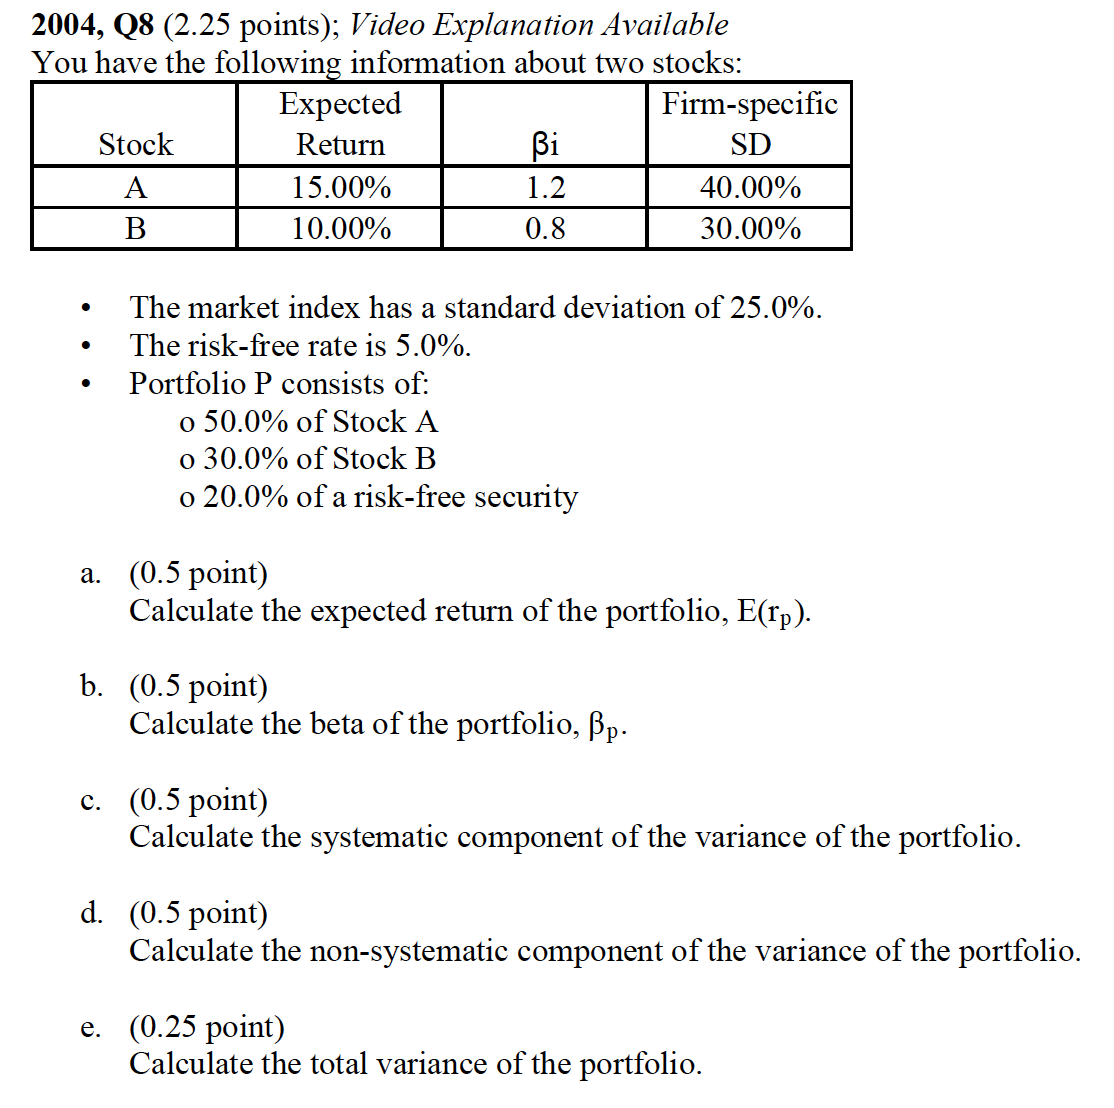
\includegraphics{Section A/questions/2004-8Q.png}
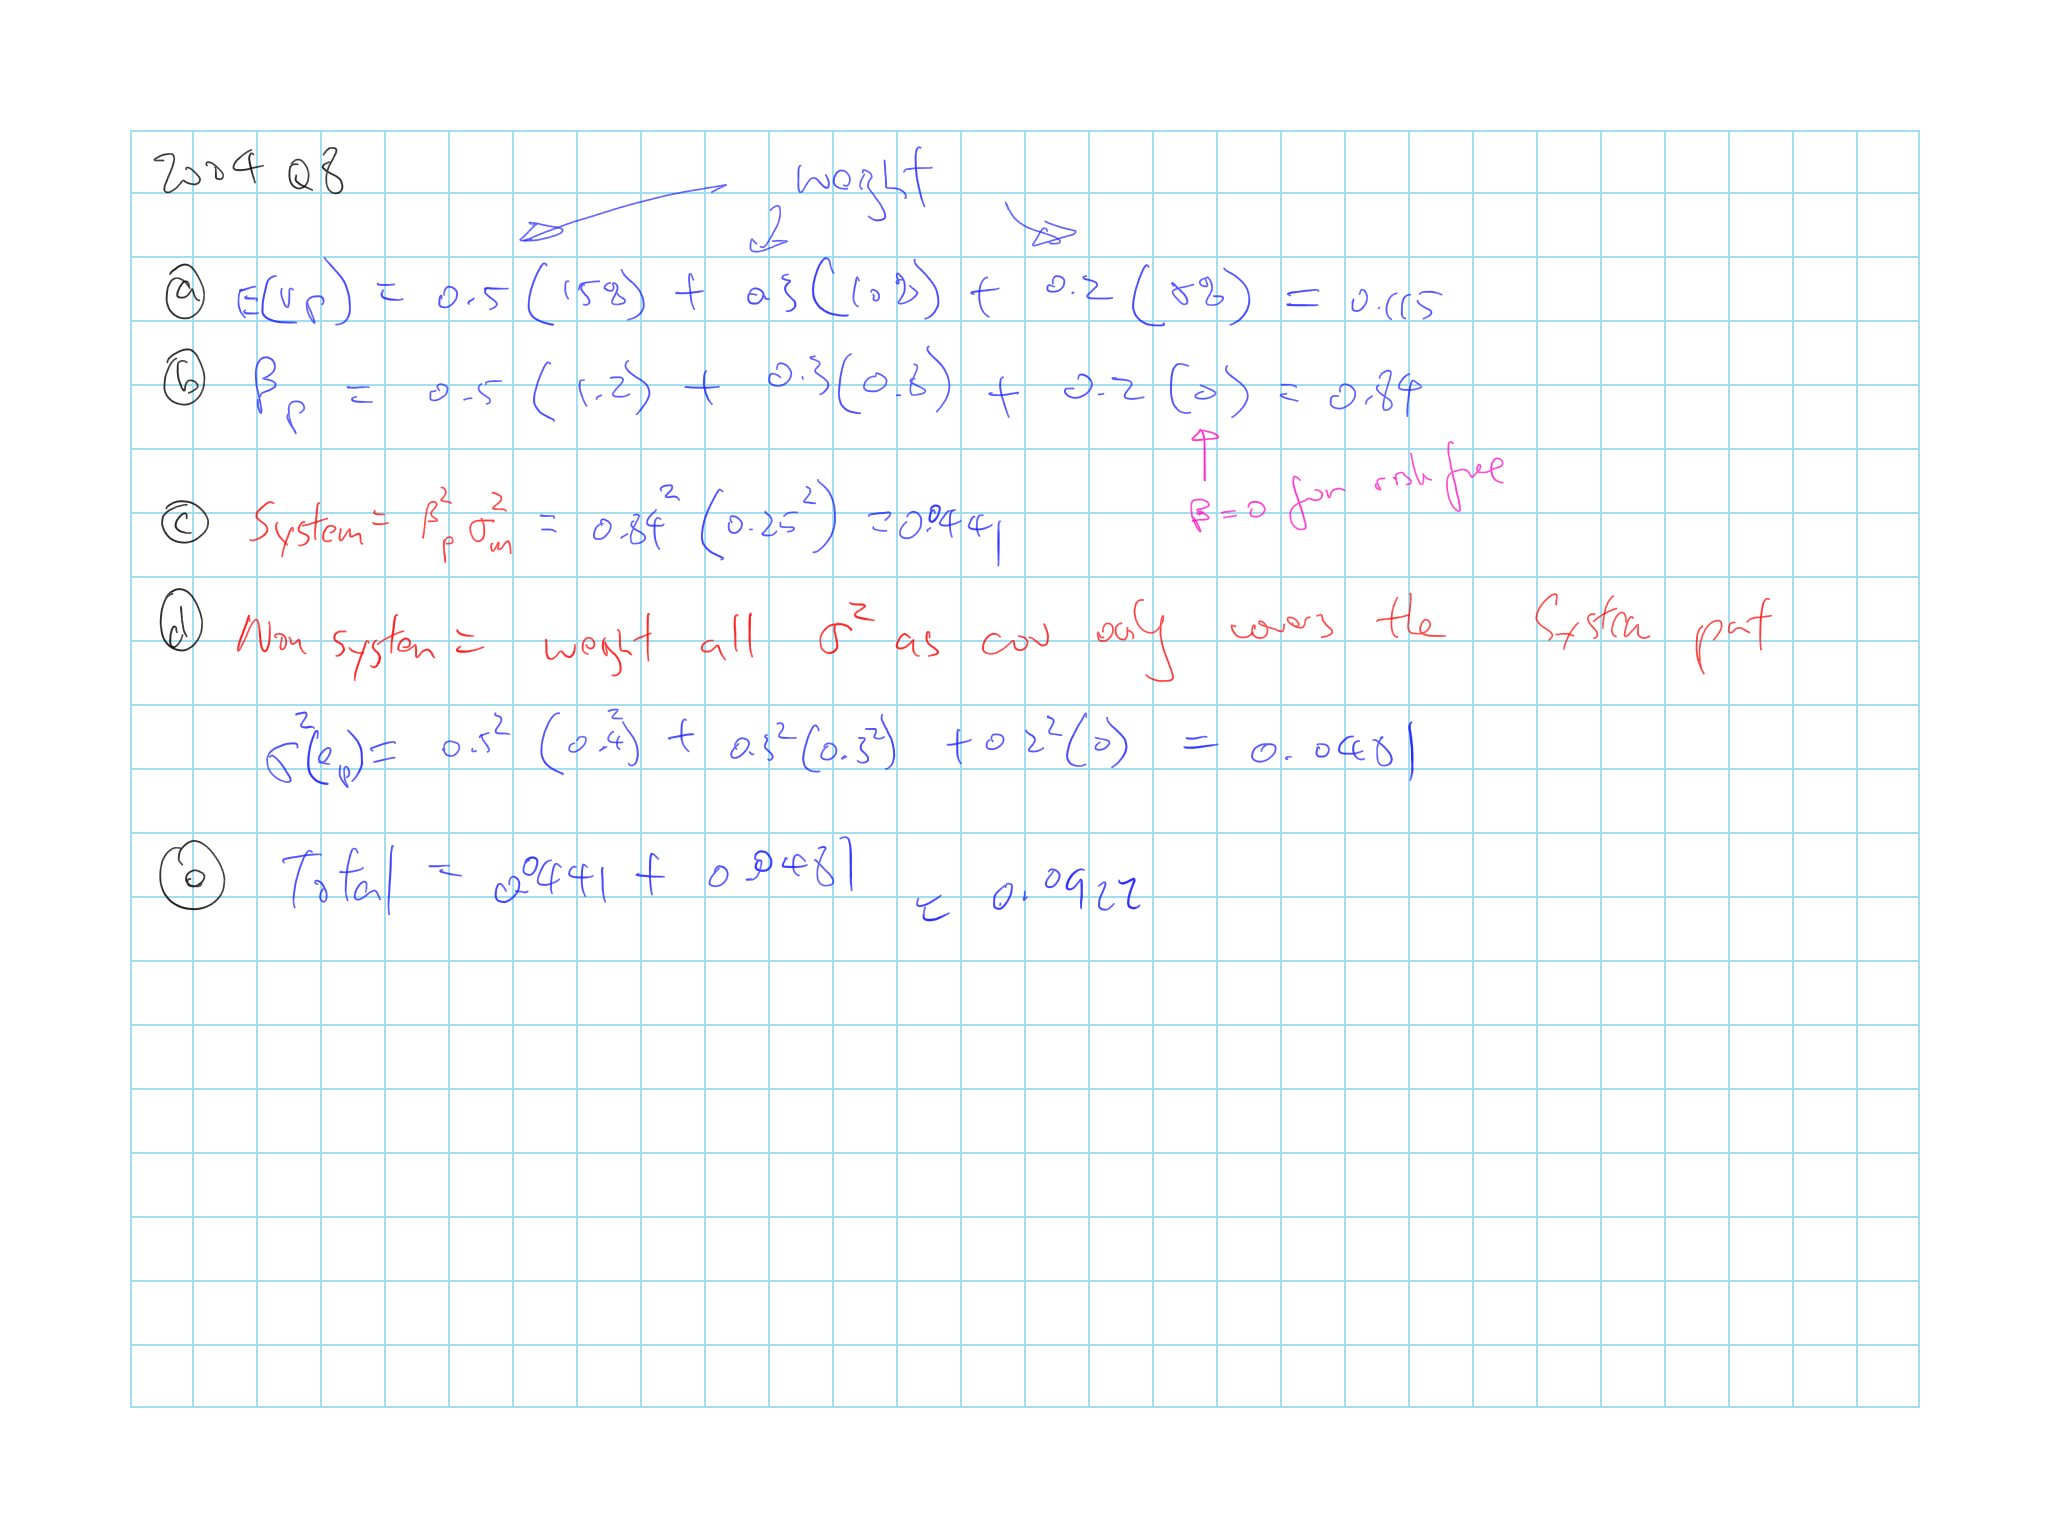
\includegraphics{Section A/questions/2004-8A.png}

 2013, Q3 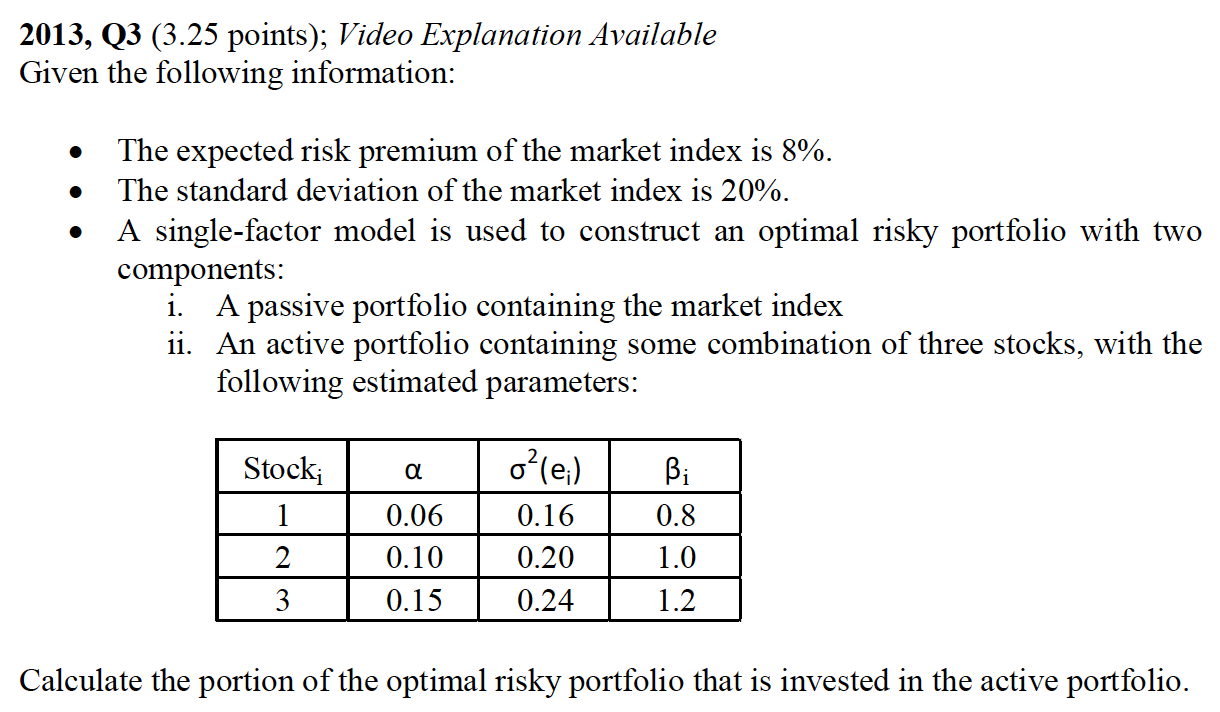
\includegraphics{Section A/questions/2013-3Q.png}
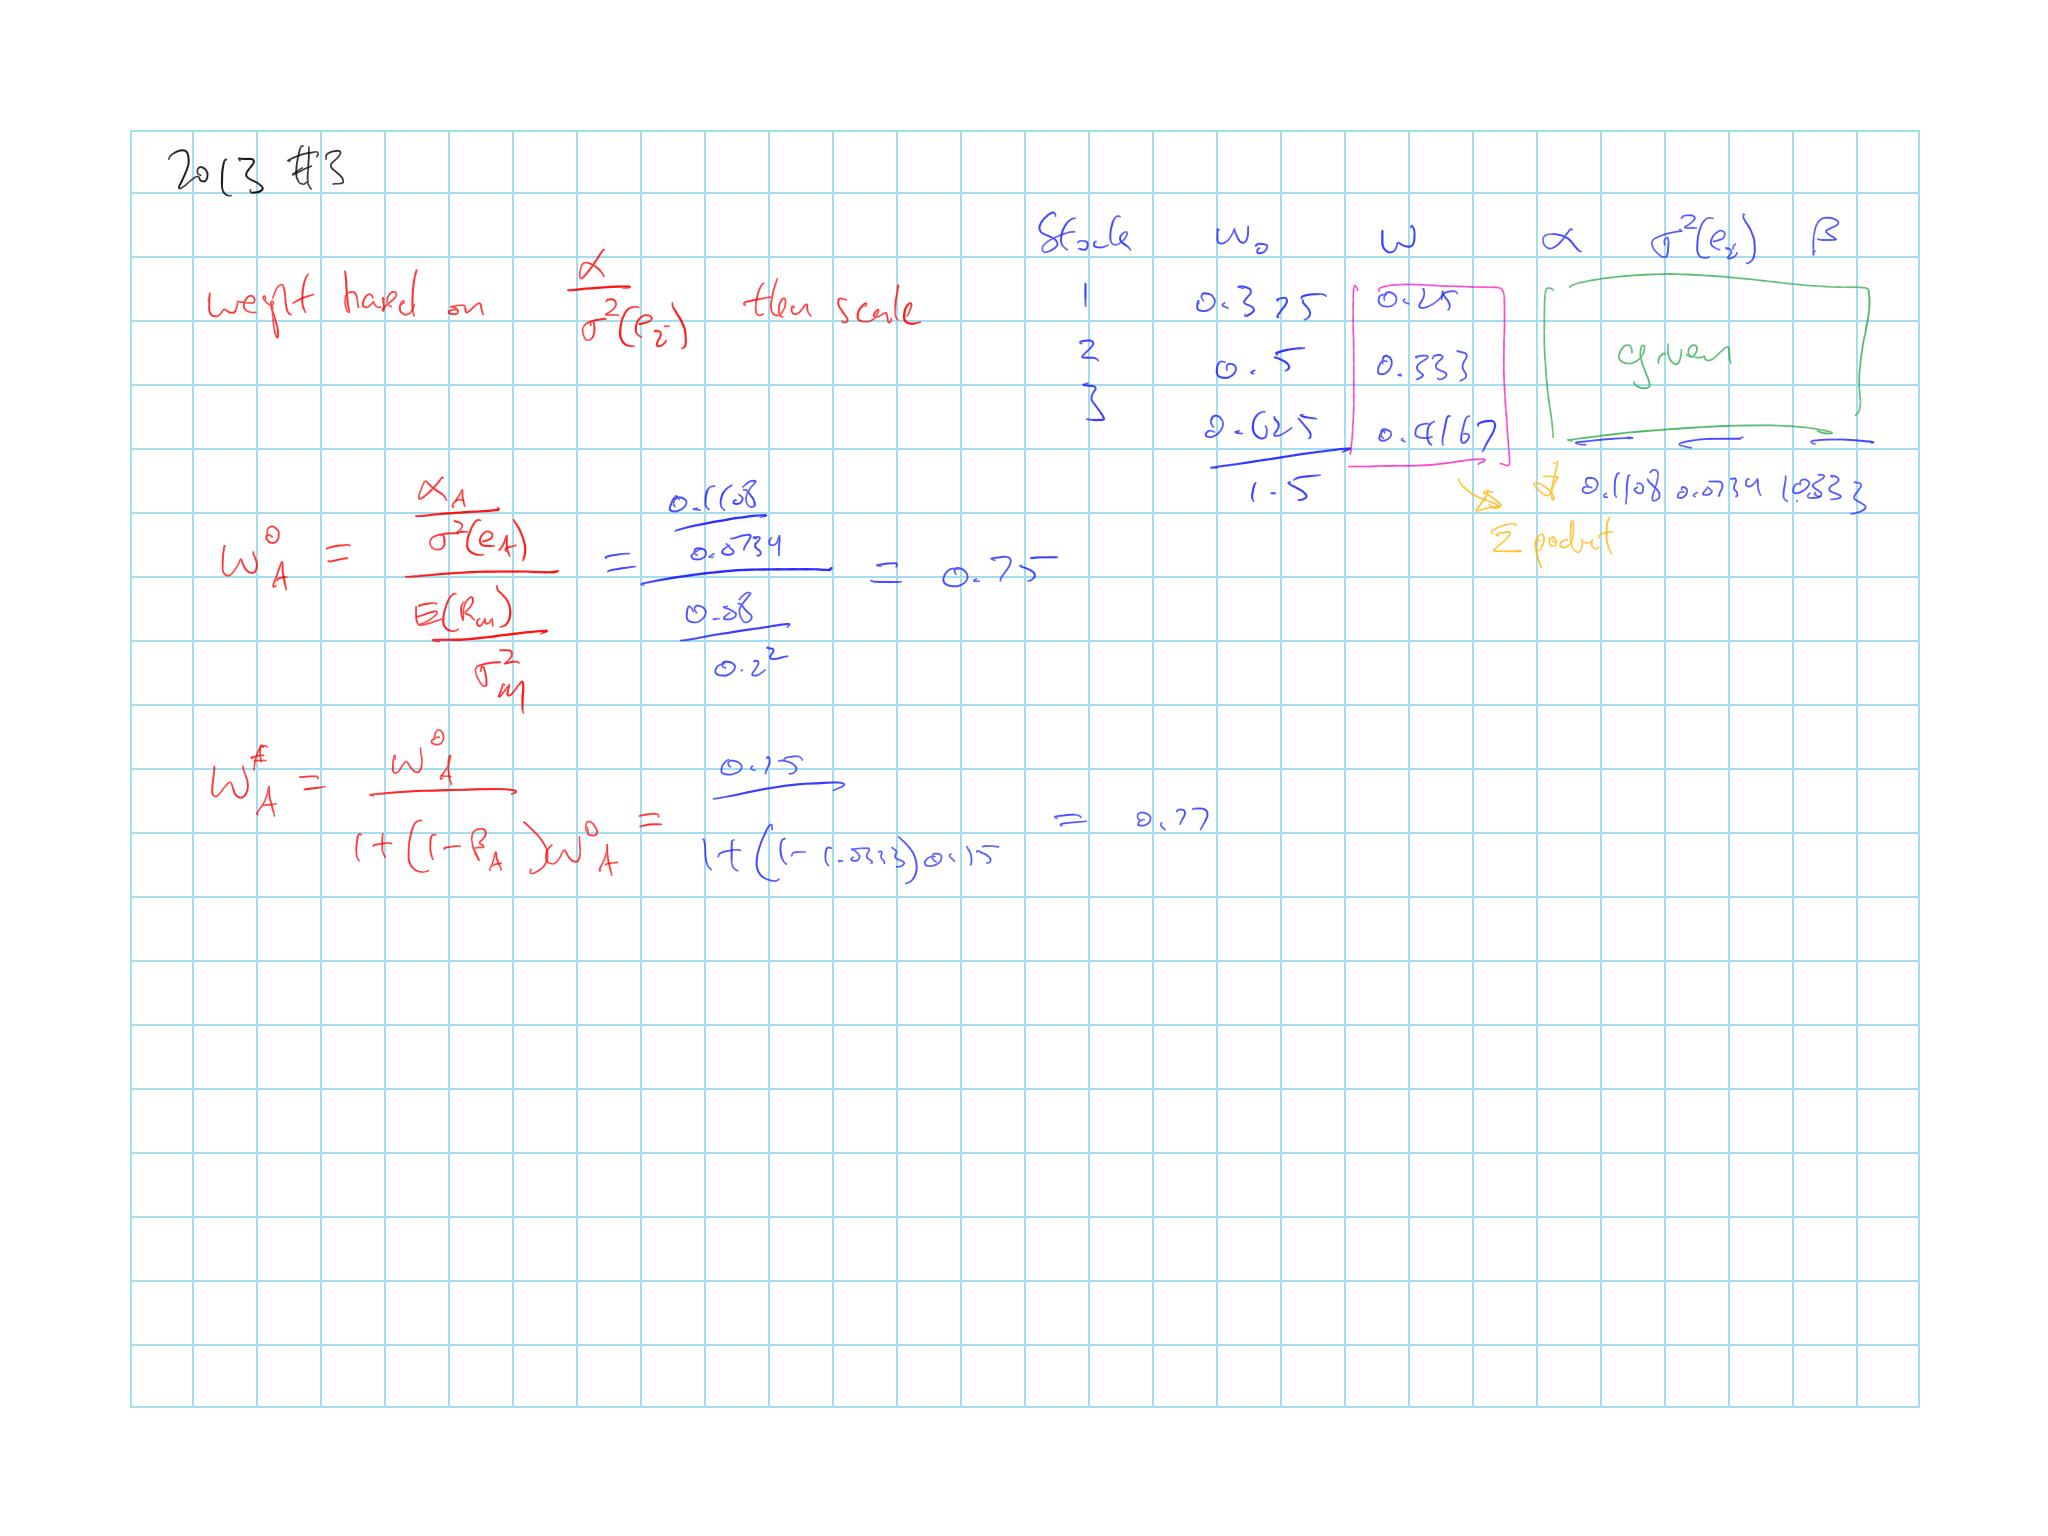
\includegraphics{Section A/questions/2013-3A.png}

 2015, Q3 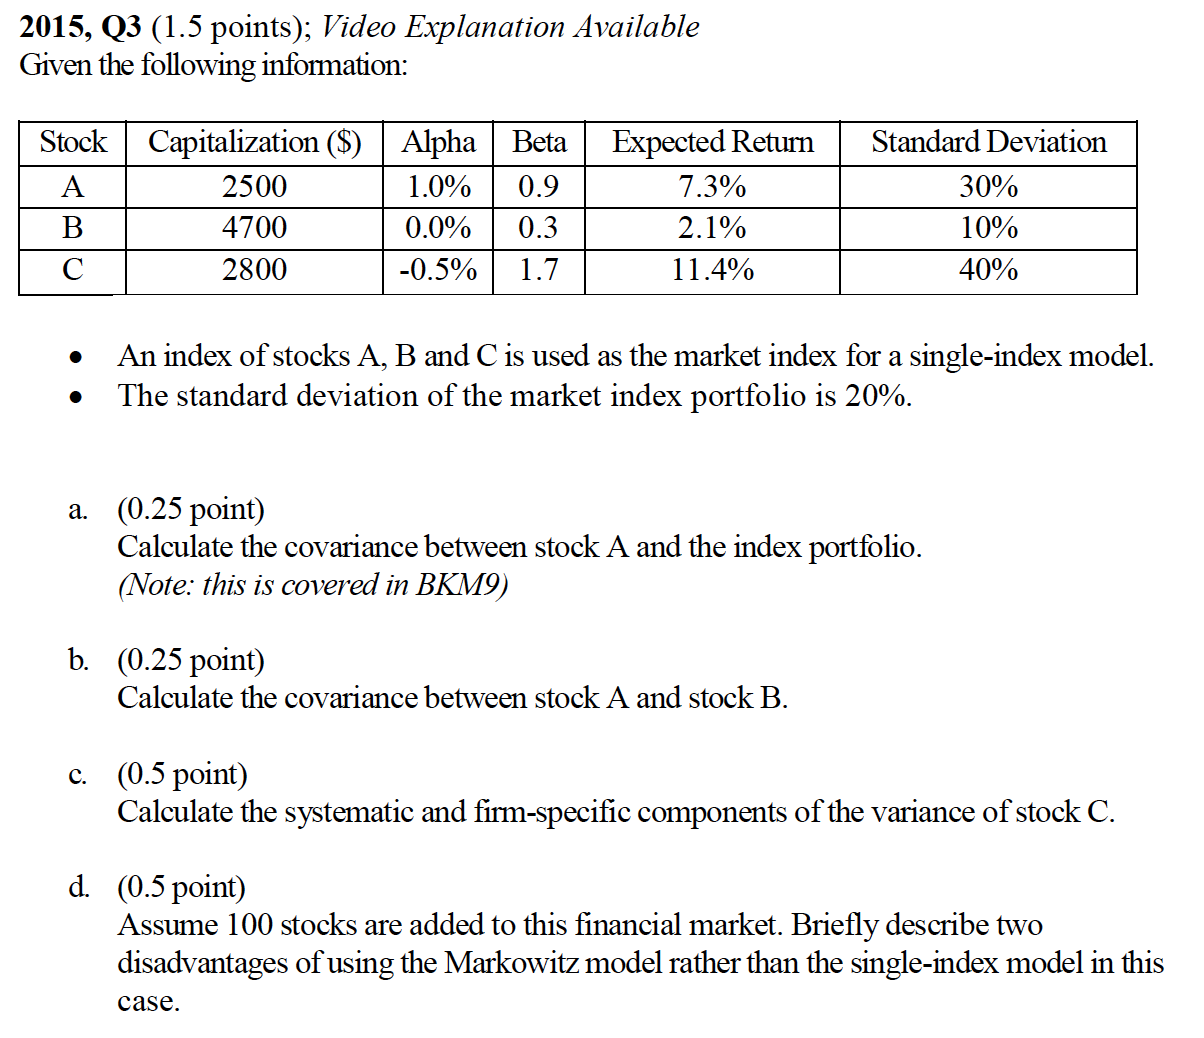
\includegraphics{Section A/questions/2015-3Q.png}
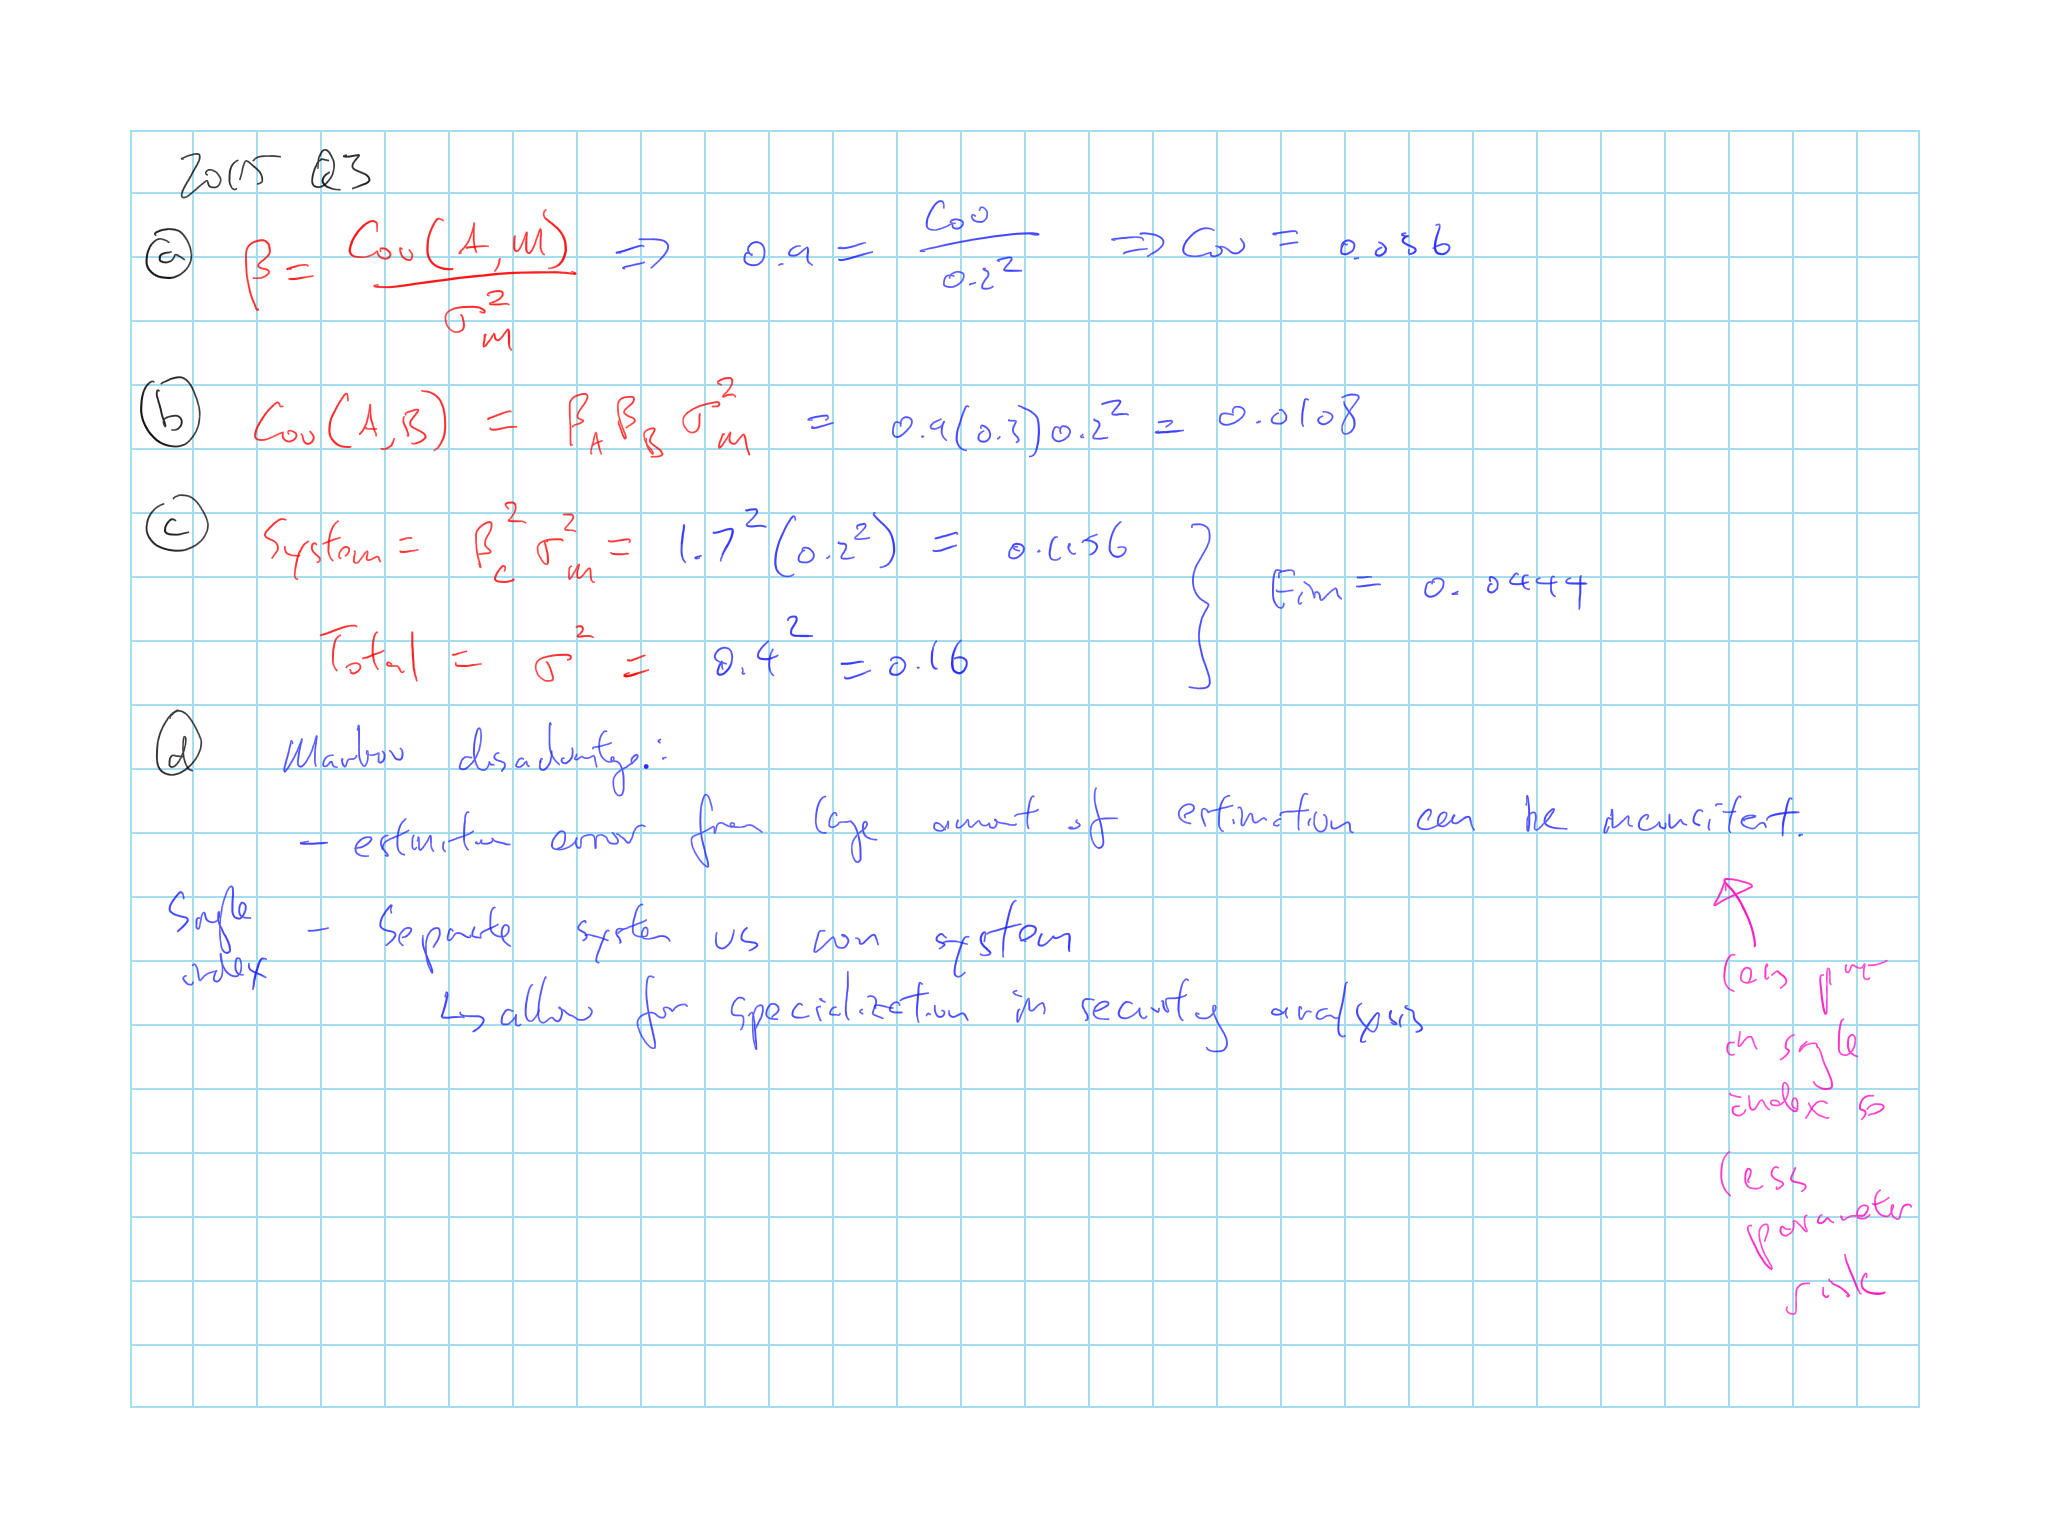
\includegraphics{Section A/questions/2015-3A.png}

\chapter{A4 BKM9: Capital Asset Pricing
Model}\label{a4-bkm9-capital-asset-pricing-model}

Z. Bodie, A. Kane, A. Marcus

\section{Cliff's Summary}\label{cliffs-summary-3}

Know the CAPM assumptions

\begin{itemize}
\tightlist
\item
  \protect\hyperlink{behav-ass}{Behavioral assumptions}
\item
  \protect\hyperlink{market-ass}{Market assumptions}
\end{itemize}

Normative (test assumptions) and positive (examines prediction) model
testing

Be familiar of the CAPM proof

\protect\hyperlink{SML}{SML} (and compare to CML)

CAPM test and \protect\hyperlink{CAPM-test-caveat}{caveats} to the
results

\textbf{CAPM Extensions}

Zero \(\beta\)

\begin{itemize}
\tightlist
\item
  Slopt of \(SML_{zb} < SML_{reg}\)
\end{itemize}

Non-traded assets

\begin{itemize}
\item
  Portfolio of traded assets that hedge the private business will be bid
  up \(\Rightarrow\) (-) \(\alpha\) under standard CAPM
\item
  Labor intensive firms will have lower demand \(\Rightarrow\) (+)
  \(\alpha\) in traditional CAPM
\end{itemize}

Multiperiod CAPM

\begin{itemize}
\item
  Hedge portfolios on the additional sources of risk to arise from
  longer horizon will be bid up

  \begin{itemize}
  \tightlist
  \item
    Assets that have higher return during periods of adverse economic
    environment will be bid up
  \item
    Bid up prices of assets that hedge the increases in prices of
    consumption goods (inflation protection)
  \end{itemize}
\end{itemize}

Consumption CAPM

\begin{itemize}
\item
  Assets with (+) covariance with consumption growth (higher payoff when
  consumption is already high) are viewed as riskier \(\Rightarrow\)
  Risk premium higher
\item
  \(\operatorname{E}[R_i] = \beta_{iC}RP_C\)
\end{itemize}

Liquidity Adjustment

\begin{itemize}
\item
  Demand additional return on liquidity risk
\item
  Can be adjusted with liquidity \(\beta\) that reflects the sensitivity
  of the return of the security to changes in market liquidity
\end{itemize}

\subsection{Types of Exam Questions}\label{types-of-exam-questions-3}

{Haven't done TIA practice questions}

\textbf{Concepts}

\begin{itemize}
\tightlist
\item
  2002, Q11: meaning of the \(\beta\)
\item
  2003, Q11: draw stock with (+) \(\alpha\) with the SML
\item
  2004, Q5: CAPM assumptions
\item
  2004, Q7: zero \(\beta\) CAPM
\item
  2008, Q3: Interpretation of plot of XS stock return vs XS market and
  also variability around the line
\item
  2010, Q4: CAPM assumptions on wealth, tax, human capital (ignored, not
  public), future cash flow expectations(homogenous), portfolio
  selection (MV optimizers)
\item
  2011, Q3: \(\alpha\) should center around 0 in a bunch of stocks
\item
  \(\star\) 2013, Q4: impact of selling market portfolio and by single
  stock with \(\beta = 0.75\)

  \begin{itemize}
  \tightlist
  \item
    Reduce systematic risk but significant increase non systematic risk,
    risk increase over all
  \item
    Expected return should fall as well as CAPM dictates that return
    only rewards systematic risk
  \end{itemize}
\item
  2014, Q3: Empirical and implied SML and that for stock above the SML
  is a better buy
\end{itemize}

\textbf{Calculations}

\begin{itemize}
\tightlist
\item
  2005, Q8: Calculate \(\beta\) based on quarterly return of stock and
  market
\item
  2005, Q12: back out numbers with CAPM
\item
  \(\star\) 2006, Q6: Back out \(\beta\) then \(\alpha\) then SML

  \begin{itemize}
  \tightlist
  \item
    Assume there is \(\alpha\) is the expected return is based on
    analysis
  \item
    Need to assume equal change of scenarios for the \(\alpha\) to make
    sense?
  \end{itemize}
\item
  \(\star \star\) \protect\hyperlink{2015-4}{2015, Q4}: Long questions

  \begin{itemize}
  \tightlist
  \item
    Expected return
  \item
    Arbitrage with 0 variance portfolio
  \end{itemize}
\item
  \(\star\) 2015, Q5: zero beta CAPM, assumptions and properties
\end{itemize}

\textbf{Plug and Play}

\begin{itemize}
\tightlist
\item
  2003, Q10: return of a portfolio (sum up the \(\beta\)'s)
\item
  2004, Q6: return of a stock with CAPM
\item
  2011, Q4: return of stock with CAPM
\end{itemize}

\section{Introduction}\label{introduction-1}

\textbf{CAPM}

Shows the relationship between risk and expected return in equilibrium

\textbf{Assumes}:

\begin{itemize}
\item
  All investors optimized portfolio using Markowitz procedure
  \(\Rightarrow\) Construct efficient frontier based on all available
  risky assets \(\Rightarrow\) Identify efficient risky portfolio P
\item
  Investors face an identical investable universe and same input list to
  construct efficient frontier \(\Rightarrow\) Same weights for each
  risky asset
\item
  Since market portfolio is based on the same risky portfolios, it will
  have the same weights \(\Rightarrow\) Investor will hold the market
  portfolio \(\Rightarrow\) CAL = CML
\end{itemize}

\textbf{Mutual fund theorm}: All investors hold a common risky
portfolio, they would have no problem if all the stock in the market
were replaced with shares of a single mutual fund holding the market
portfolio

Key implications:

\begin{itemize}
\item
  Market portfolio is efficient
\item
  Premium on a risky asset is \(\propto\) its \(\beta\)
\end{itemize}

\section{CAPM Assumptions}\label{capm-assumptions}

 \textbf{Individual Behavior Assumptions}

\begin{itemize}
\item
  Investors are rational mean-variance optimizers

  \begin{itemize}
  \tightlist
  \item
    Not concerned about correlation of asset return with inflation/
    prices of consumption items
  \end{itemize}
\item
  Single period planning horizon (can alter later)

  \begin{itemize}
  \item
    Longer periods would result in extra-market risk factors
  \item
    e.g. \(\Delta\) interest rates \(\downarrow\) income \(\Rightarrow\)
    Assets that can hedge this will be priced higher
  \end{itemize}
\item
  Identical input list

  \begin{itemize}
  \tightlist
  \item
    Implies that all information are public
  \end{itemize}
\item
  There are many investors and they are all price takers

  \begin{itemize}
  \tightlist
  \item
    Transactions have no impact on the price
  \end{itemize}
\item
  Investors have homogeneous expectations

  \begin{itemize}
  \tightlist
  \item
    Everyone's analysis come to the same conclusion
  \end{itemize}
\end{itemize}

 \textbf{Market Structure Assumptions}

\begin{itemize}
\item
  All assets are publicly traded (can alter later) and short positions
  are allowed

  \begin{itemize}
  \tightlist
  \item
    Assets have to be tradable for investors to be able to derive
    identical input list
  \end{itemize}
\item
  Can borrow/lend at a common risk free rate (can alter later)

  \begin{itemize}
  \tightlist
  \item
    Necessary for investors to derive the same tangency portfolio
  \end{itemize}
\item
  All information is publicly available
\item
  No taxes

  \begin{itemize}
  \tightlist
  \item
    Different tax rate \(\Rightarrow\) Different after tax rates on the
    same stock \(\Rightarrow\) Investor could derive different after tax
    optimal risky portfolio
  \end{itemize}
\item
  No transaction costs
\end{itemize}

\subsection{Assumptions Testing}\label{assumptions-testing}

\textbf{Model Testing}

\begin{itemize}
\item
  Normative: test model assumptions
\item
  Positive: examines the predictions
\end{itemize}

Impossible to create a model consistent with the complexity of markets
\(\Rightarrow\) CAPM is a simplification of reality

\(\hookrightarrow\) Ideally assumptions will be robust (outcome not
highly sensitive to the violation of the assumptions)

\subsection{Derivation of CAPM}\label{derivation-of-capm}

Proved:

\begin{itemize}
\item
  Contribution of an individual stock to the portfolio risk premium is
  \(w_i[\operatorname{E}[r_i]-r_f]\)
\item
  Contribution of an individual stock the portfolio variance is
  \(w_i \operatorname{Cov}(r_i, r_M)\)
\end{itemize}

\textbf{Reward-to-risk ratio} based on above:

\(\dfrac{\text{Contribution to Risk Premium}}{\text{Contribution to Variance}} = \dfrac{w_i[\operatorname{E}[r_i]-r_f]}{w_i \operatorname{Cov}(r_i, r_M)} = \dfrac{[\operatorname{E}[r_i]-r_f]}{\operatorname{Cov}(r_i, r_M)}\)

Reward-to-risk ratio for \emph{market portfolio} is the \textbf{market
price of risk}:

\(\dfrac{[\operatorname{E}[r_M]-r_f]}{\sigma^2_M}\)

In equilibrium all securities should have the same reward-to-risk ratio
\(\Rightarrow\) reward-to-risk ratio for individual stock = market price
of risk:

\(\begin{array}{ccc}  \dfrac{[\operatorname{E}[r_i]-r_f]}{\operatorname{Cov}(r_i, r_M)} &= \dfrac{[\operatorname{E}[r_M]-r_f]}{\sigma^2_M} \\  \operatorname{E}[r_i] &= r_f + \beta_i [\operatorname{E}[r_M] - r_f] &\text{where } \beta_i = \dfrac{\operatorname{Cov}(r_i, r_M)}{\sigma^2_M} \\ \end{array}\)

\subsection{Security Market Line}\label{security-market-line}

\(\beta\) measures the risk of the security

\begin{itemize}
\tightlist
\item
  Can be estimated by plotting XS return on stock vs XS return on market
\item
  Intercept should be 0
\end{itemize}

 \textbf{Security Market Lines}\\
Graphs relationship between \(\beta\) and \(\operatorname{E}[r]\) of a
stock

\begin{figure}[htbp]
\centering
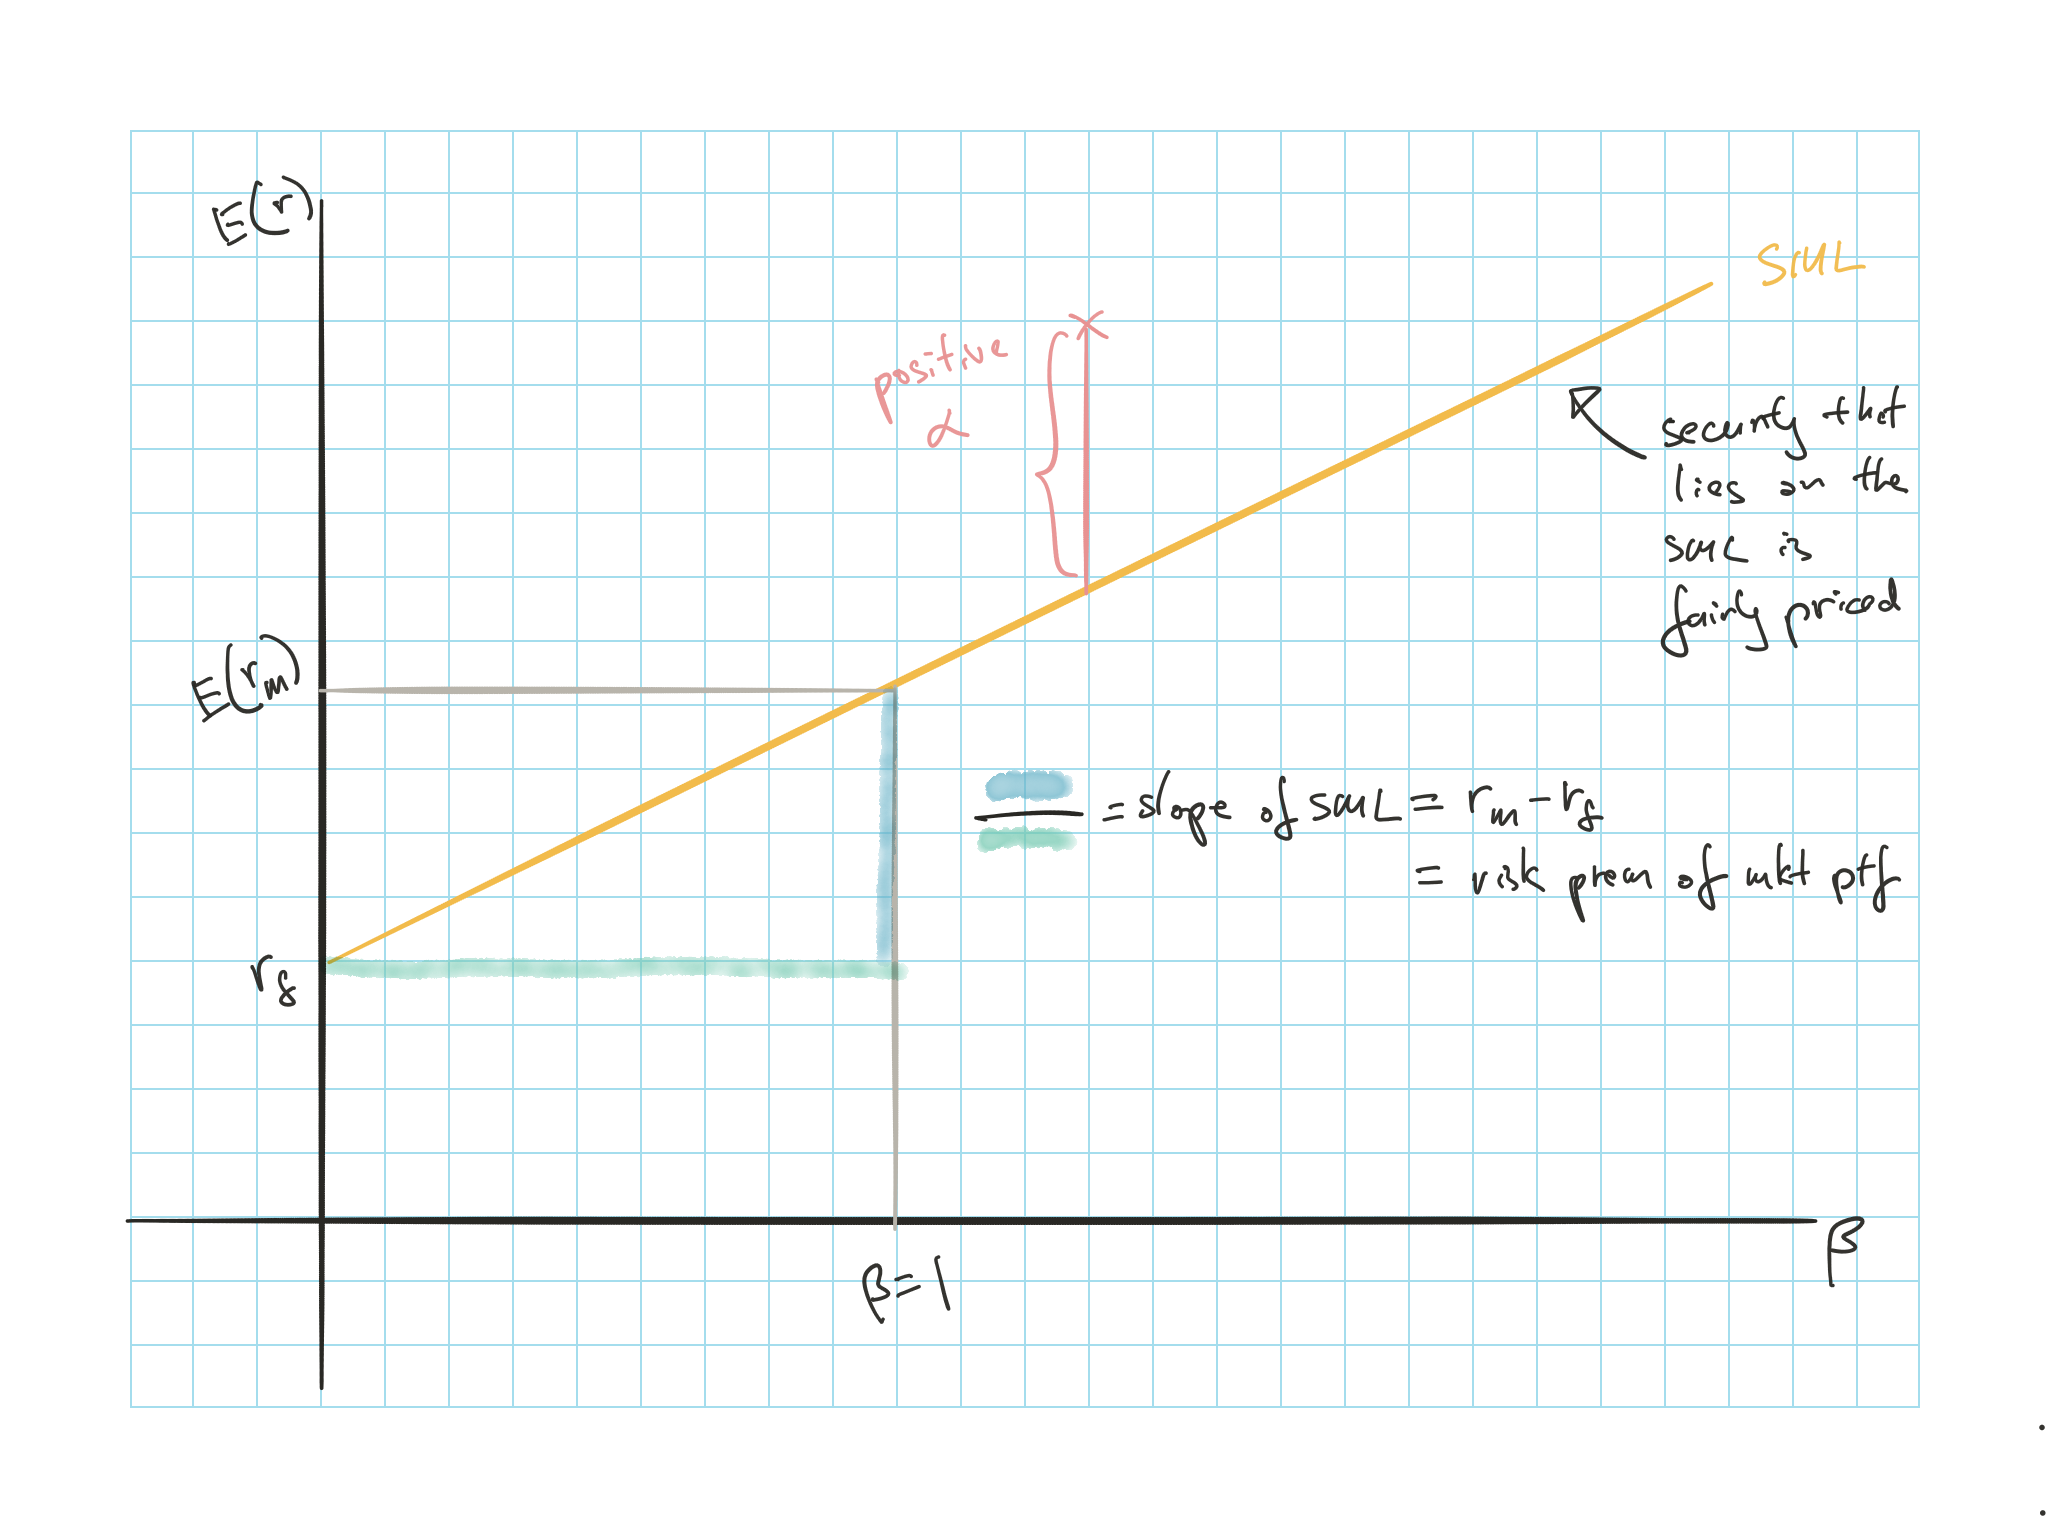
\includegraphics{figures/Exam 9 - 9.png}
\caption{alt text}
\end{figure}

\textbf{SML vs CML}

\begin{itemize}
\item
  CML: Risk premium of \emph{efficient Portfolios} vs \(\sigma\)

  \begin{itemize}
  \tightlist
  \item
    \(\sigma\) is the appropriate risk measure for portfolios
  \end{itemize}
\item
  SML: Risk premium of \emph{individual asseets} vs \(\beta\)

  \begin{itemize}
  \tightlist
  \item
    \(\beta\) is the appropriate risk measure for individual securities
    held as part of a well diversified portfolio
  \end{itemize}
\end{itemize}

\subsection{Testing CAPM}\label{testing-capm}

Impossible to construct market portfolio, so test the SML equation
instead \(\operatorname{E}[R_i] = \beta_i R_M\)

Regression on the XS returns of a sample of stocks against their betas
over time

\(R_{i,t} = \lambda_0 + \lambda_1 \beta_i + \lambda_2 \sigma^2(e_i) + \eta_{i,t}\)

CAPM predicts:

\begin{itemize}
\item
  \(\lambda_0 = 0\) as the average \(\alpha = 0\)
\item
  \(\lambda_1 = R_M\) as the slope of SML = market risk premium
\item
  \(\lambda_2 = 0\) as the risk premium is only based on proportion of
  market risk premium
\end{itemize}

Estimate the \(\beta\) and residual variance for each stock from time
series of stock return

 \textbf{Caveat}

\begin{itemize}
\item
  Parameter estimates have large errors and may be correlated
  \(\Rightarrow\) Downward bias in \(\lambda_1\) and upward bias on
  \(\lambda_0\)
\item
  Might reject CAPM even if it is valid

  \begin{itemize}
  \tightlist
  \item
    Returns simulated following CAPM but regression still indicates that
    CAPM does not hold
  \end{itemize}
\item
  Parameters are time varying but the regression techniques does not
  recognize this
\end{itemize}

\section{CAPM Extensions}\label{capm-extensions}

Problematic assumptions:

\begin{itemize}
\item
  No restrictions on short sales, but in reality it can be difficult to
  take short positions
\item
  All assets are tradable
\item
  No transaction costs
\item
  Single period horizon
\end{itemize}

However the extensions of CAPM are not perfect so none have superseded
CAPM so far

\subsection{Zero Beta CAPM}\label{zero-beta-capm}

When investors face borrowing restrictions of risk free asset

\(\operatorname{E}[r_i] = \operatorname{E}[r_Z] + \beta_i \left[\operatorname{E}[r_M] - \operatorname{E}[r_Z]\right]\)

\begin{itemize}
\item
  \(Z\) = zero-beta portfolio for M
\item
  Uncorrelated portfolio on the inefficient side of the minimum-variance
  frontier
\end{itemize}

Investors with borrowing restrictions will invest more in high \(\beta\)
stocks and less in low \(\beta\) \(\Rightarrow\) \(\uparrow\) price of
high \(\beta\) stocks

\begin{itemize}
\item
  Slopt of \(SML_{zb} < SML_{reg}\)
\item
  Risk premium on the market portfolio is smaller as the
  \(\operatorname{E}[r_Z] > r_f\) so less reward for bearing risk
\end{itemize}

\subsection{Non-Traded Assets}\label{non-traded-assets}

Some assets are tradable e.g.~human capital and privately held business

\begin{itemize}
\tightlist
\item
  These are of significant values and can have a material impact on the
  equilibrium returns of traded securities
\end{itemize}

\textbf{Privately held business}

\begin{itemize}
\item
  Privately held business w/ similar characteristics to traded assets:\\
  Little impact to CAPM as owners can still achieve diversification by
  reducing their portfolio of other similar traded assets
  \(\Rightarrow\) Still holding market portfolio
\item
  Privately held business w/o similar characteristics to traded
  assets:\\
  Portfolio of traded assets that hedge the private business will be up
  \(\Rightarrow\) \(\downarrow\) expected return \(\Rightarrow\)
  \(-\alpha\) in traditional CAPM
\end{itemize}

\textbf{Human Capital}

\begin{itemize}
\item
  Only way to hedge is for employees to avoid purchasing share of their
  own employer \(\Rightarrow\) labor intensive firms will have lower
  demand \(\Rightarrow\) \(+\alpha\) in traditional CAPM
\item
  Adjusted CAPM for labor income:

  \begin{itemize}
  \item
    \(\operatorname{E}[R_i] = \operatorname{E}[R_M] \dfrac{\operatorname{Cov}(R_i, R_M) + \frac{P_H}{P_M}\operatorname{Cov}(R_i, R_H)}{\sigma^2_M + \frac{P_H}{P_M}\operatorname{Cov}(R_M,R_H)}\)
  \item
    \(P_H\): value of aggregate human capital
  \item
    \(P_M\): market value of traded assets
  \end{itemize}
\item
  Adjustment produce lower \(\beta\) so a SML with a less steep slope,
  which explain negative alpha of high beta securities indicated by some
  tests
\end{itemize}

\subsection{Multiperiod CAPM}\label{multiperiod-capm}

\textbf{Intertemporal CAPM}

Assume investors will optimize their consumption/ investment over their
lifetime

ICAPM = CAPM when:

\begin{itemize}
\item
  Only type of risk is the uncertainty about portfolio returns
\item
  Investment opportunities are constant over time
\end{itemize}

However, over the long run we expect additional sources of risk to arise
and \textbf{hedge portfolios} will be bid up

\begin{enumerate}
\def\labelenumi{\arabic{enumi})}
\item
  Changes in the parameters that describe investment opportunities

  \begin{itemize}
  \tightlist
  \item
    Investors will bid up prices of assets that have higher return
    during periods of adverse economic environment \(\Rightarrow\) lower
    expected return
  \end{itemize}
\item
  Changes in the prices of consumption goods

  \begin{itemize}
  \tightlist
  \item
    Investors will bid up prices of assets that hedge the increases in
    prices of consumption goods (inflation protection)
  \end{itemize}
\end{enumerate}

ICAPM with \(K\) sources of extramarket risk and \(K\) hedge portfolios:

\(\operatorname{E}[R_i] = \beta_{iM}\operatorname[R_M] + \sum_k \beta_{ik}\operatorname[R_k]\)

\begin{itemize}
\tightlist
\item
  \(\beta_{ik}\) is the \(\beta\) on the \(k\)\textsuperscript{th} hedge
  portfolio
\end{itemize}

\subsection{Consumption Based CAPM}\label{consumption-based-capm}

Assume that in a period, investors need to allocate the current wealth
between consumption today and savings/ investments to support future
consumption

Optimal mix: utility from an additional dollar of consumption today =
utility associated with the future consumption generated from the
investment of that dollar

\begin{itemize}
\tightlist
\item
  Additional income from savings are more valued during tough economic
  times (w/ limited consumption opportunities) \(\Rightarrow\) Assets
  with (+) covariance with consumption growth (higher payoff when
  consumption is already high) are viewed as riskier \(\Rightarrow\)
  Risk premium higher
\end{itemize}

CCAPM:

\(\operatorname{E}[R_i] = \beta_{iC}RP_C\)

\begin{itemize}
\item
  \(C\) is a consumption tracking portfolio, one with the highest
  correlation with consumption growth
\item
  \(\beta\) of market portfolio can be \textgreater{} 1
\end{itemize}

Disadvantages: consumption growth figures are published infrequently and
with significant error

\subsection{Liquidity Adjusted CAPM}\label{liquidity-adjusted-capm}

Security prices should be discounted to reflect illiquidity

\begin{itemize}
\item
  Standard CAPM ignores liquidity costs like bid-ask spread
\item
  Discount \(\uparrow\) as trading cost \(\uparrow\) but \emph{not}
  proportional to the increase due to \textbf{clientele effect}

  \begin{itemize}
  \tightlist
  \item
    Frequent traders hold more liquid assets and long term traders hold
    less liquid assets
  \end{itemize}
\end{itemize}

Investor also demand additional return on liquidity risk (risk of
unanticipated changes in liquidity)

\begin{itemize}
\tightlist
\item
  Can be adjusted with liquidity \(\beta\) that reflects the sensitivity
  of the return of the security to changes in market liquidity
\end{itemize}

\section{Past Exam Questions}\label{past-exam-questions-3}

 2015, Q4 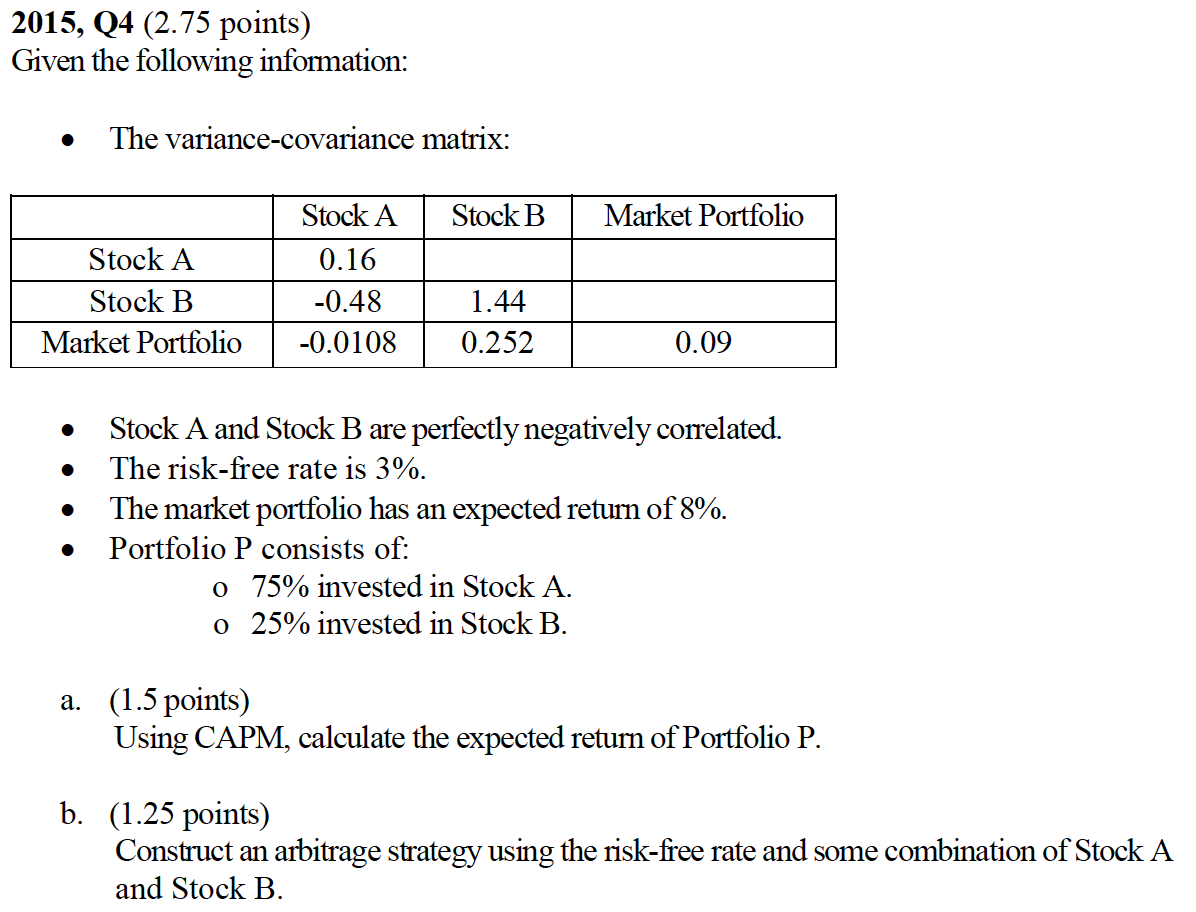
\includegraphics{questions/2015-4Q.png}
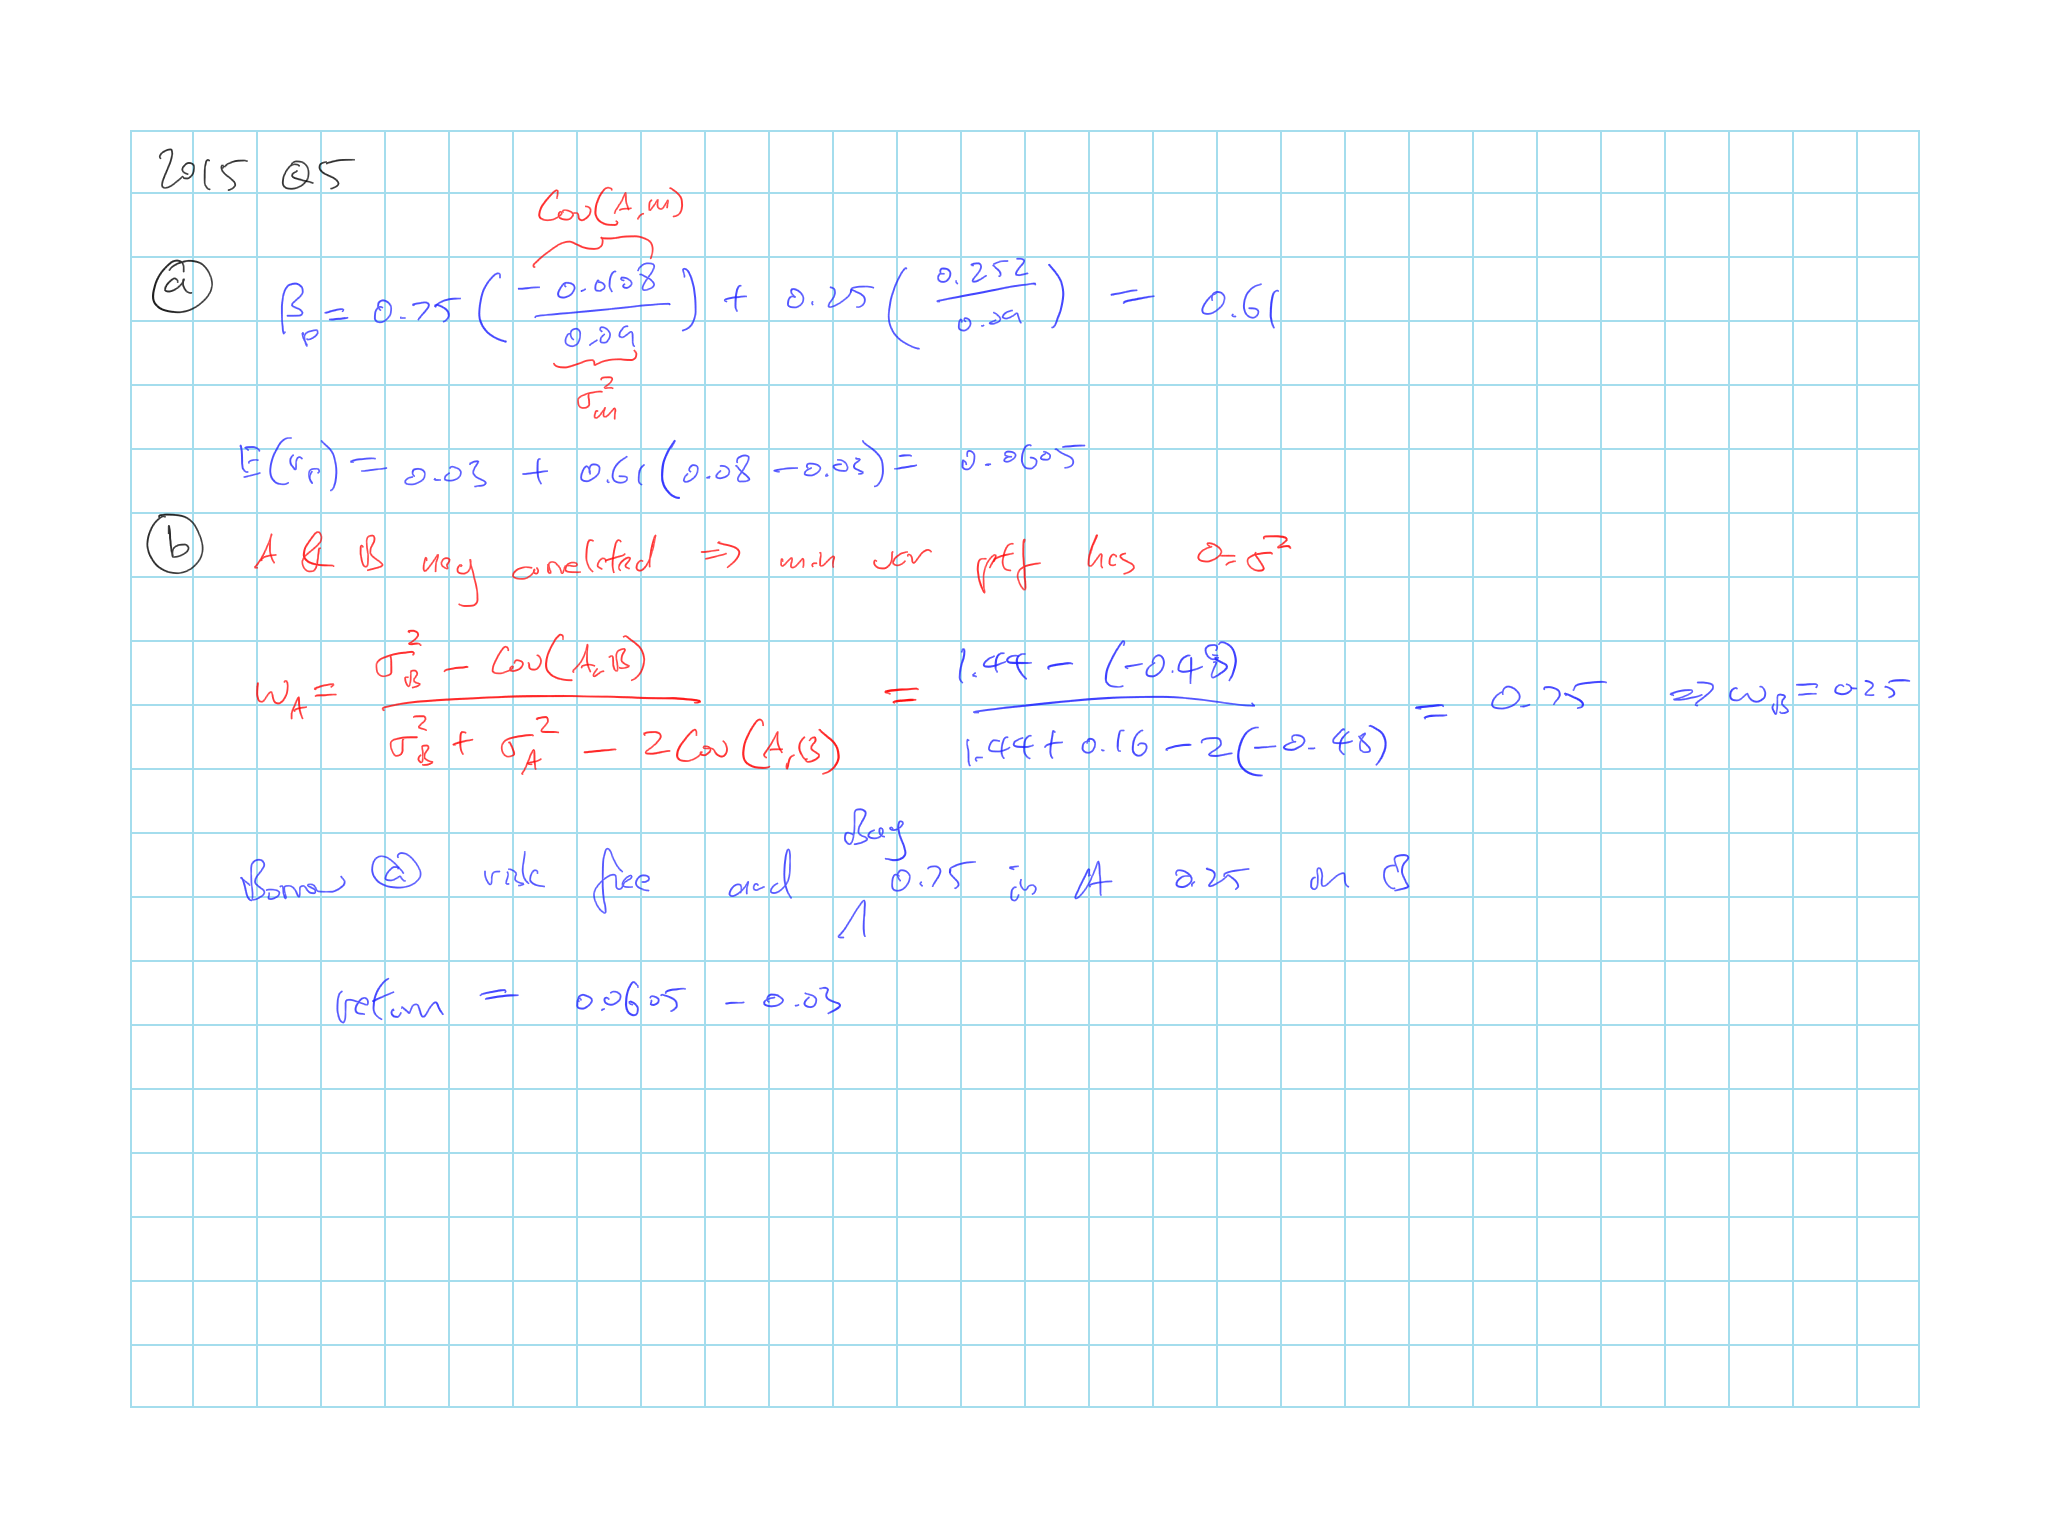
\includegraphics{questions/2015-4A.png}

\chapter{A5 BKM10: Arbitrage Pricing
Theory}\label{a5-bkm10-arbitrage-pricing-theory}

Z. Bodie, A. Kane, A. Marcus

\section{Cliff's Summary}\label{cliffs-summary-4}

Factor model (single, multi)

\begin{itemize}
\tightlist
\item
  Multifactor SML (how is this derived?)
\end{itemize}

\protect\hyperlink{famma}{Fama French Three Factor}

\begin{itemize}
\tightlist
\item
  Small minus big stocks
\item
  High minus low book:market ratio
\item
  Market index
\item
  The formula adds the \(\alpha\) instead of \(r_f\) like CAPM
\end{itemize}

\textbf{Arbitrage}:\\
Opportunity to earn 1) risk-less profit 2) without need to make a net
investment

\textbf{Law of one price}:\\
Two assets with equivalent economical aspects should have the same
market price

\textbf{APT Assumptions}:

\begin{enumerate}
\def\labelenumi{\arabic{enumi})}
\item
  Security returns can be described by a factor model
\item
  There are a sufficient number of securities to diversify away
  idiosyncratic risk
\item
  Well functioning securities markets do not allow for persistence of
  arbitrage opportunities
\end{enumerate}

2 ways to reach \protect\hyperlink{equil}{equilibrium}

Know how to execute an arbitrage opportunity

\protect\hyperlink{APT-v-CAPM}{APT vs CAPM}

\protect\hyperlink{TB}{Treynor Black Model} for optimal risky if
arbritrage is identified so not to be over exposed to residual risk

\subsection{Types of Exam Questions}\label{types-of-exam-questions-4}

{Haven't done TIA practice questions}

\textbf{Concepts}

\begin{itemize}
\tightlist
\item
  2006, Q9: Famma French additional factors
\item
  \(\star\) 2011, Q2: arbitrage equilibirum; risk return dominance
\item
  \(\star\) \protect\hyperlink{2015-6}{2015, Q6}: FF model and
  behavioral
\end{itemize}

\textbf{Arbitrage opportunity}

\begin{itemize}
\tightlist
\item
  2000, Q13: structure an arbitrage opportunity
\item
  2003, Q13 b: structure arbitrage
\end{itemize}

\textbf{Factor Model}

\begin{itemize}
\tightlist
\item
  2001, Q32: expected XS return and weighted \(\beta\)
\item
  2003, Q13 a: expected return
\item
  2004, Q9: arithmetic to back out factors from 2 equations
\item
  2006, Q7: factor model arithmetic
\item
  2008, Q4: factor model arithmetic
\item
  2009, Q4: factor model arithmetic
\end{itemize}

\section{Factor Models}\label{factor-models}

Similar to the index model but focus on individual risks rather than
using market as proxy

\begin{itemize}
\tightlist
\item
  Index model implicitly assumes that the security has the same relative
  sensitivity to each risk factor that is represented by \(M\)
\end{itemize}

\subsection{Single Factor Model}\label{single-factor-model-1}

Recall from BKM8, return based on a single factor \(F\):

\(r_i = \operatorname{E}[r_i] + \beta_i F + e_i\)

\begin{itemize}
\item
  \(F\): deviation of a factor from is expected value
\item
  \(\beta_i\) sensitivity of the security return to the factor
\end{itemize}

\subsection{Multifactor Model}\label{multifactor-model}

Add additional factors to account for varying sensitivities to different
factors

\(r_i = \operatorname{E}[r_i] + \sum \limits_{j=1}^n \beta_{ij} F_j + e_i\)

Impact of actual return = \(\beta_i F\) where \(F\) is the actual -
expected

\subsubsection{Multifactor SML}\label{multifactor-sml}

Calculate the risk premiums for the risk factors with a \textbf{factor
portfolio}

\begin{itemize}
\tightlist
\item
  Portfolio that have \(\beta = 1\) for which the risk premium is being
  measured, else \(\beta = 0\)
\end{itemize}

\(\operatorname{E}[r_i] = r_f + \sum \limits_{j=1}^n \beta_{ij} \left( \operatorname{E}[r_j] -r_f \right)\)
{Where is this from?}

\subsection{Fama French Three Factor
Model}\label{fama-french-three-factor-model}

Uses firm characteristics that seem to be proxy for exposure to
systematic risk

\(R_{it} = \alpha_i + \beta_{iM}R_{Mt} + \beta_{iSMB}SMB_t + \beta_{iHML}HML_t + e_{it}\)

\begin{itemize}
\item
  \(SMB\) = return of a portfolio of small stocks in XS of portfolio of
  large stocks
\item
  \(HML\) = return of a portfolio of high
  \(\frac{\text{book}}{\text{market}}\) in XS of portfolio of low
  \(\frac{\text{book}}{\text{market}}\) stocks
\item
  Include market index as well to include systematic risk from
  macroeconomic factors
\end{itemize}

The 2 additional factors maybe acting as proxies for something
fundamental

\begin{itemize}
\item
  Measure some of the systematic risk not captured by only using the
  market portfolio
\item
  F-F not necessarily thought small firms or high B:M had better returns
\end{itemize}

\textbf{Problem with FF model}: It is derived from empirical evidence,
and none of the factors can be identified as hedging a specific source
of uncertainty

\begin{itemize}
\tightlist
\item
  Pattern might be purely due to chance
\end{itemize}

\section{Arbitrage Pricing Theory}\label{arbitrage-pricing-theory}

\textbf{Arbitrage}:\\
Opportunity to earn 1) risk-less profit 2) without need to make a net
investment

\textbf{Law of one price}:\\
Two assets with equivalent economical aspects should have the same
market price

\textbf{APT Assumptions}:

\begin{enumerate}
\def\labelenumi{\arabic{enumi})}
\item
  Security returns can be described by a factor model
\item
  There are a sufficient number of securities to diversify away
  idiosyncratic risk
\item
  Well functioning securities markets do not allow for persistence of
  arbitrage opportunities
\end{enumerate}

\subsection{Equilibrium}\label{equilibrium}

Market prices change to eliminate arbitrage opportunities and reach
equilibrium when the opportunity disappears

\textbf{Risk return dominance}\\
Many investors will make limited changes to their portfolio (depending
on risk aversion) and the cumulative changes from sufficient volumes
move the market price

\textbf{Arbitrage}\\
Investor who discovers the arbitrage will maximize his position to
maximize profits so lower number of investors are needed to move prices
back to equilibrium

\subsection{Impact of Diversification}\label{impact-of-diversification}

Return of portfolio with \(n\) stocks using single factor model
\(r_p = \operatorname{E}[r_p] + \beta_p F + e_p\)

\(\sigma^2(e_p) = \dfrac{\sigma^2(e_i)}{n}\) \(\Rightarrow\)
\(\underbrace{\lim \limits_{n \rightarrow \infty} \sigma^2(e_p) = 0}_{\text{diversification}}\)

\(\hookrightarrow\) After diversification
\(r_p = \operatorname{E}[r_p] + \beta_p F\) as the non factor risk can
be diversified away and security will only receive risk premium for the
factor risk

\begin{figure}[htbp]
\centering
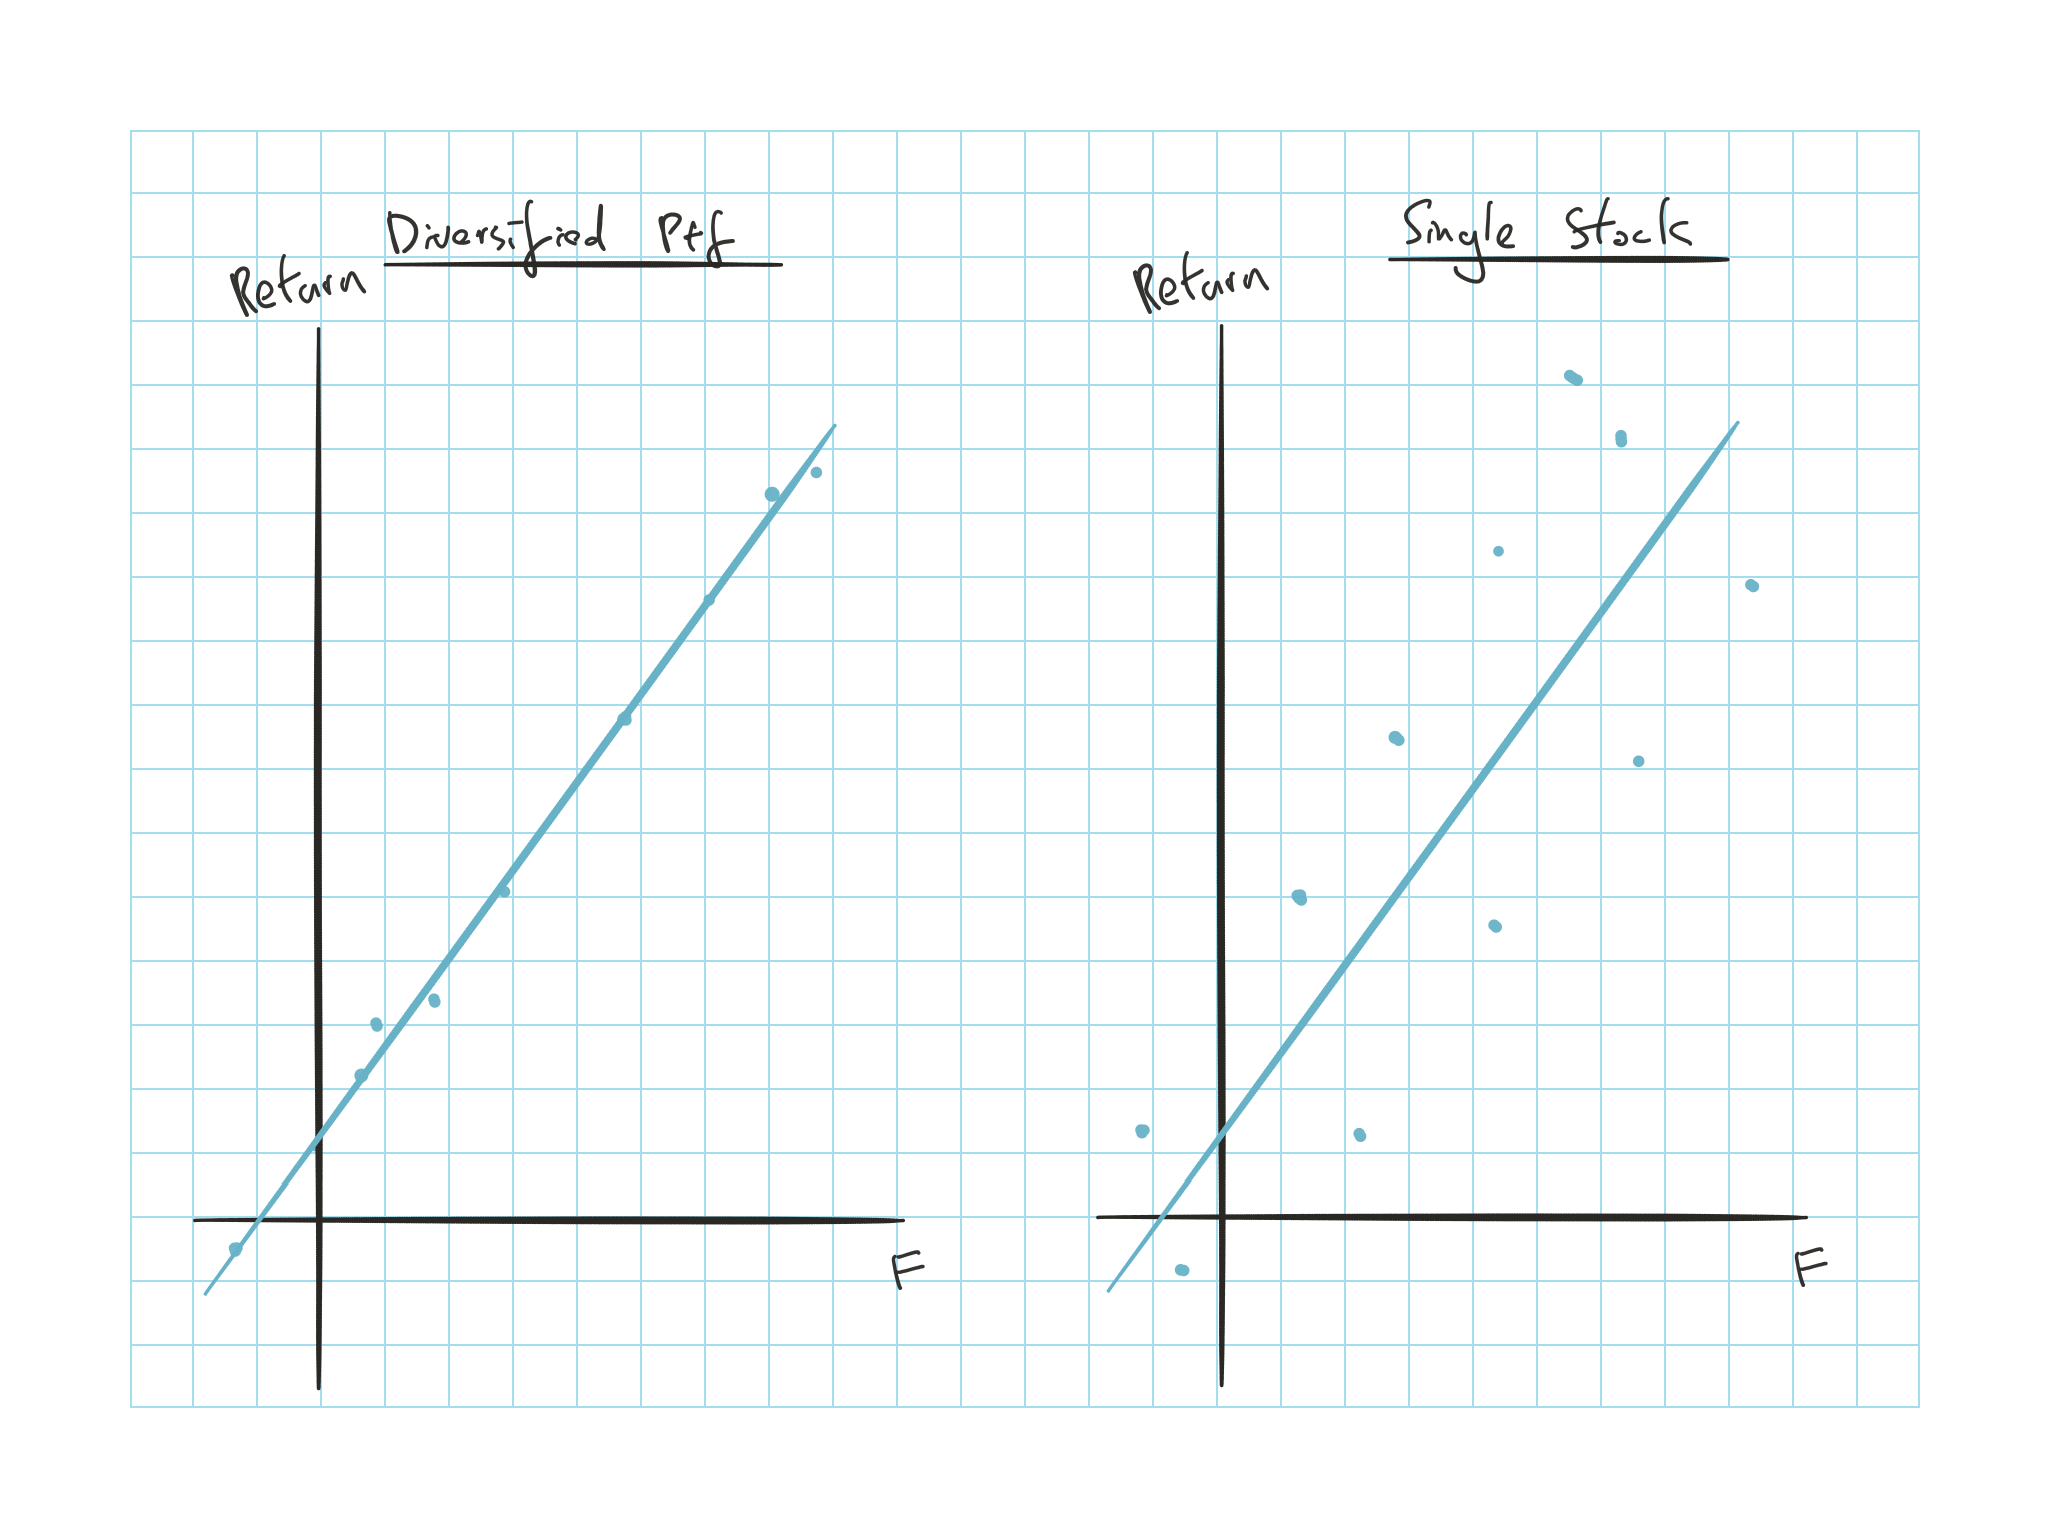
\includegraphics{figures/Exam 9 - 10.png}
\caption{alt text}
\end{figure}

\subsection{Executing Arbitrage}\label{executing-arbitrage}

Given 2 well diversified portfolio \(M\) and \(P\) that has (+)
\(\alpha\)

Construct \(Z\) a zero beta portfolio with \(M\) and \(P\)

\(\beta_Z = w_p \beta_p + (1-w_p)\beta_M = 0\) \(\Rightarrow\)
\(w_p = \dfrac{1}{1-\beta_p}\)

\(\hookrightarrow\) \(Z\) is riskless since no residual risk from
diversification and 0 systematic risk from \(\beta\)

\(\operatorname{E}[R_z] = \alpha_Z = w_p \alpha_p = \dfrac{\alpha_p}{1 - \beta_p}\)

\begin{itemize}
\item
  If \(\beta_p < 1\), borrow money and invest in \(Z\) to make a risk
  free profit
\item
  If \(\beta_p > 1\), short \(Z\) and invest in risk free
\end{itemize}

\subsection{No-Arbitrage Equation}\label{no-arbitrage-equation}

Return of well diversified portfolio with APT
\(\operatorname{E}[R_p] = \alpha_p + \beta_p \operatorname{E}[R_M]\)

\(\Downarrow\) No arbitrage, \(\alpha = 0\)

APT SML: \(\operatorname{E}[R_p] = \beta_p \operatorname{E}[R_M]\)

\begin{itemize}
\tightlist
\item
  Same as CAPM SML
\end{itemize}

For APT, there can not be 2 parallel APT SML as that would mean one to
be dominant over the other and investor can produce arbitrage
opportunity

\subsection{APT vs CAPM}\label{apt-vs-capm}

Disadvantages:

\begin{itemize}
\item
  Based on diversified portfolio \(\Rightarrow\) 0 residual risk
\item
  If residual risk is sufficiently high, cannot have full confidence in
  APT
\end{itemize}

Advantages:

\begin{itemize}
\item
  Does not reply on mean-variance optimizers assumption
\item
  Does not require an all inclusive portfolio
\end{itemize}

\subsection{Optimization in a Single Index
Market}\label{optimization-in-a-single-index-market}

APT indicates how to generate infinite profit if risk premium of well
diversified portfolio differs from the SML

\begin{itemize}
\tightlist
\item
  If arbitrage portfolio not perfectly well diversified, increasing the
  size of an investment to take advantage of an arbitrage opportunity
  will also increase the risk of the arbitrage position
\end{itemize}

 \textbf{Treynor-Black Model}

To construct an optimal risky portfolio based on identified underpriced
asset or portfolio under a single factor market

\begin{itemize}
\item
  Model produces an optimal risky portfolio if there is residual risk
\item
  More flexible that APT in reflecting residual risk that may exist
\end{itemize}

\section{Past Exam Questions}\label{past-exam-questions-4}

 2015, Q6 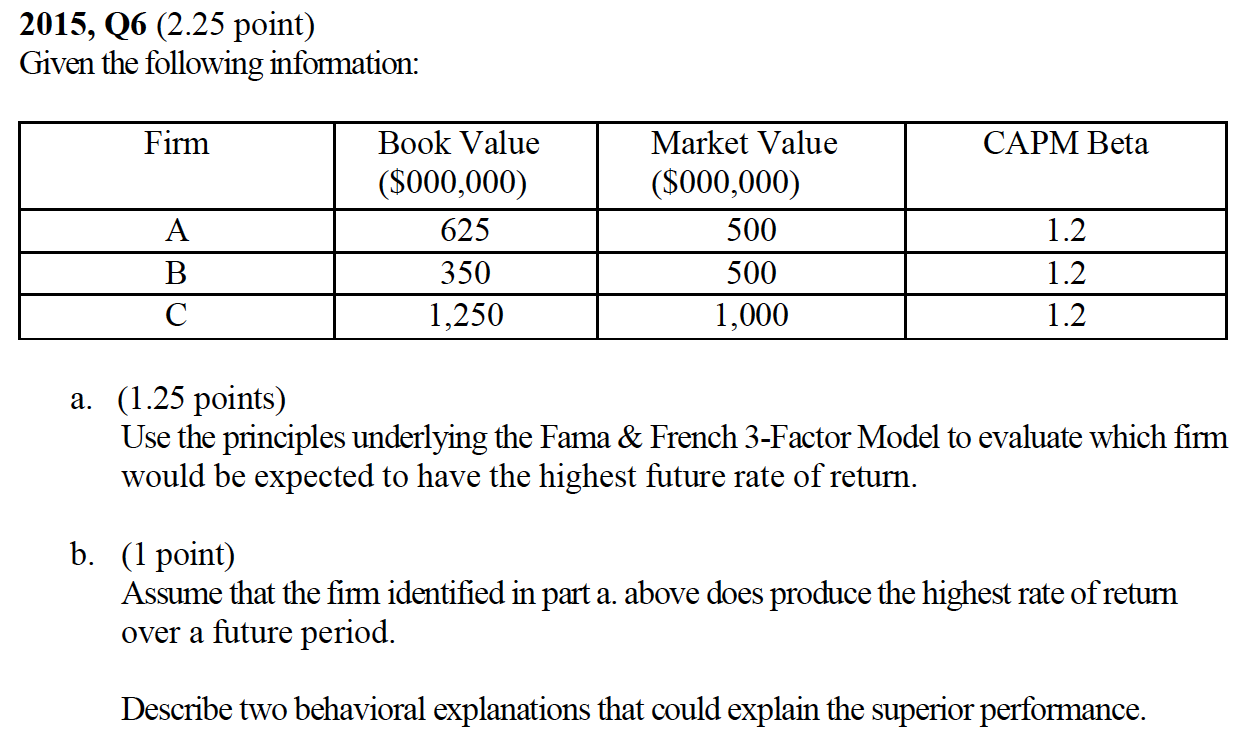
\includegraphics{questions/2015-6Q.png}

\begin{enumerate}
\def\labelenumi{\alph{enumi}.}
\item
  Ignore \(\beta\) since it's the same; A because highest B:M value and
  lower MV
\item
\end{enumerate}

\begin{itemize}
\tightlist
\item
  Small firm ignored by large investors due to regret avoidance, require
  higher return due to less information and unconventional choice
\item
  Forecast error, more weight in recent performance of glamour firm
\item
  Smaple size neglect, tend to infer too quickly and extrapolate price
  of low B:V too high
\end{itemize}

\chapter{A6 BKM11: Efficient Market
Hyothesis}\label{a6-bkm11-efficient-market-hyothesis}

Z. Bodie, A. Kane, A. Marcus

\section{Cliff's Summary}\label{cliffs-summary-5}

3 \protect\hyperlink{EMH-forms}{forms} of EMH and
\protect\hyperlink{EMH-implications}{implications}

Event studies and the \protect\hyperlink{event-diff}{difficulties}

\protect\hyperlink{efficient-diff}{Difficulties} in assessing whether
the market is efficient

\begin{itemize}
\item
  Also the test should be risk adjusted which is also difficult
\item
  \protect\hyperlink{EMH-3-forms-test}{Test} for the 3 forms of EMH

  \begin{itemize}
  \tightlist
  \item
    Efficient market anomalies
  \end{itemize}
\item
  Interpretation might be difficult too
\item
  There is still perpose for portfolio management
\end{itemize}

Look at performance of stock analyst and also mutual fund managers

\subsection{Types of Exam Questions}\label{types-of-exam-questions-5}

{Haven't done TIA practice questions}

\textbf{Concepts}

\begin{itemize}
\tightlist
\item
  2003, Q14: passive investment strategy and why is it better under EMH
\item
  2003, Q15: Small firm in jan and B:M ratio anomalies
\item
  2004, Q10: 3 EMH; Technical analysis; EMH implication; ptf managment
  purpose
\item
  2006, Q8: Anomalies
\item
  2007, Q5: semi-strong, anomalies
\item
  2008, Q5: 3 EMH; price drift violate semi strong
\item
  2008, Q7: Should not be persistent performance
\item
  2010, Q1: value of portfolio managment; if everyone actually use the
  passive portfolio not price correction will happen
\item
  \(\star\) \protect\hyperlink{2012-3}{2012, Q3}: 3 form of EMH;
  examples
\item
  \(\star\) {[}2014, Q6{]}(\#2014-6: market anomalies based on data
\end{itemize}

\section{Introduction}\label{introduction-2}

Stock prices should reflect all available information

New information relevant to the stock will cause the price to change and
since new information is unpredictable, so is the movement of stock
price (random walk process)

 3 versions of EMH

\begin{itemize}
\item
  \textbf{Weak form}: Reflect all information that can be derived from
  examining market (trading) data
\item
  \textbf{Semi-strong form}: Reflect all publicly available information
  about the firm's prospects
\item
  \textbf{Strong form}: Reflect all information relevant to the firm
  including non-public information
\end{itemize}

All 3 versions pertain only to information available

\section{Implication of EMH}\label{implication-of-emh}

If EMH holds, it'll impact the following investment strategies

\subsection{Technical Analysis}\label{technical-analysis}

Technical analysis search for predictable patterns of stock prices to
used to derive a profit from trading

Rely on sluggish response of the stock price to fundamental factors and
exploit the trend

\begin{itemize}
\tightlist
\item
  Uses metrics such as: \emph{Resistence levels} (levels above prices
  should not rise); \emph{Support levels} (levels below which prices
  should not fall)
\end{itemize}

Can only be successful if markets are not efficient in weak form of EMH

\subsection{Fundamental Analysis}\label{fundamental-analysis}

Uses the fundamentals of a firm to determine the appropriate prices

Try to gain insight into future performance that is not yet reflected by
the market

\begin{itemize}
\tightlist
\item
  Earning \& dividend prospects; Future interest rate expectations;
  risks
\end{itemize}

Semi-strong form of EMH states that it will not work unless investors
have a unique insight

\subsection{Active vs Passive
Managment}\label{active-vs-passive-managment}

Takes a lot of effort and cost to gain unique insight

For smaller investors cost will be \textgreater{} benefits

Should resort to passive investments or mutual funds and ETFs

EMH advocates believe that stocks are priced fairly which means buy and
sell frequently is pointless

\section{Event Studies}\label{event-studies}

 \textbf{Event study}: To determine the importance of an event by
measuring the resulting price changes

\begin{itemize}
\tightlist
\item
  Since price changes reflect new information
\end{itemize}

2 difficulties with these studies:

\begin{enumerate}
\def\labelenumi{\arabic{enumi})}
\tightlist
\item
  Market movement
\item
  Leakage
\end{enumerate}

\subsection{Market Movement}\label{market-movement}

Stock price may respond to a wide range of economic news in addition to
the event

\textbf{Abnormal return} = Actual return - benchmark return

\begin{itemize}
\tightlist
\item
  Need to calculate a proxy for what the return would have been in
  absence of the event (benchmark return)
\end{itemize}

Several methods to calculate the benchmark:

\begin{itemize}
\tightlist
\item
  Market return
\item
  Return of the stock implied by CAPM
\item
  Return of the stock implied by index model (\(e_t =\) abnormal return)
\end{itemize}

\subsection{Leakage}\label{leakage}

Information about the event maybe leaked prior and price maybe begin to
move before the event

Maybe more appropriate to measure the impact of the event by referring
to the cumulative abnormal return

\begin{itemize}
\tightlist
\item
  Beginning at a time period before the actual event is made public
\end{itemize}

\section{Are Market Efficient?}\label{are-market-efficient}

 Difficulties in determining if the markets are truly efficient:

\textbf{Magnitude Issue}: 0.1\% of a huge portfolio will be a big dollar
term contribution but very small compared to the normal volatility of
the market \(\Rightarrow\) Hard to assess how much the manager actually
contributed

\textbf{Selection Bias Issue}: Investment scheme that are known by
others will no longer generate abnormal returns \(\Rightarrow\) Only
schemes that do not work will be reported

\textbf{Lucky Event Issue}: The number of investors is so large so that
just by chance some will have to make huge returns

\subsection{Tests of Different EMH
Forms}\label{tests-of-different-emh-forms}

 Tests can be constructed for each version of EMH

\subsubsection{Weak-Form Tests}\label{weak-form-tests}

Patterns in stock returns

\textbf{Returns over short horizons}

\begin{itemize}
\item
  Measure \emph{serial correlation} of stock market returns to see
  whether investors can use historical trends to earn abnormal profits
  over the short term
\item
  Results show only small correlations over short periods

  \begin{itemize}
  \tightlist
  \item
    Exception being sectors with the best and worst returns exhibit
    stronger correlation, \emph{momentum effect}
  \end{itemize}
\end{itemize}

\textbf{Returns over long horizons}

\begin{itemize}
\item
  Similar to above but for longer term
\item
  Results show negative correlation over the long term \(\Rightarrow\)
  Fads hypothesis maybe
\item
  \(\hookrightarrow\) A contrarian investment strategy may be profitable
\end{itemize}

\begin{center}\rule{0.5\linewidth}{\linethickness}\end{center}

\subsubsection{Semi-strong Form Tests}\label{semi-strong-form-tests}

Efficient market anomalies

Investigate whether publicly available information beyond the trading
history can be used to generate abnormal returns

Results show that some easily available diagnostics can be used to
predict abnormal returns

\begin{itemize}
\item
  \textbf{Small firm in January effect}: Small firms have historically
  generate superior returns particularly in January
\item
  \textbf{Neglect firm effect}: Some firms are neglected by large
  investors so less information is available. The superior returns might
  be due to additional premium required to compensate for the risk of
  less information
\item
  \textbf{Book:Market ratios}: High B:M firm have historically
  outperformed the rest
\item
  \textbf{Post-earnings-announcement price drift}: Cumulative abnormal
  return of stocks has been shown to continue to increase even after the
  information about the even become public
\end{itemize}

Tests require the level of risk to be reflected \(\Rightarrow\) Need to
appropriately risk adjust the return, which can be more difficult than
EMH itself

\begin{center}\rule{0.5\linewidth}{\linethickness}\end{center}

\subsubsection{Strong Tests}\label{strong-tests}

Markets are not expected to be strong-form efficient, people with inside
information should be able to make superior profits

\begin{center}\rule{0.5\linewidth}{\linethickness}\end{center}

\subsection{Intrepreting the Evidence}\label{intrepreting-the-evidence}

Results above might still not be sufficient to show that the market is
inefficient:

\begin{itemize}
\item
  Properties are only proxies for fundamental determinants of risk
\item
  Properties arise just due to data mining and many of the anomalies
  disappear after discovered
\end{itemize}

\subsection{Role of Portfolio
Management}\label{role-of-portfolio-management}

Portfolio management can still be beneficial in efficient market

\begin{itemize}
\tightlist
\item
  Helps selects a diversification strategy to eliminate firm risk
\item
  Reflects tax considerations of the individual investors
\item
  Adjust portfolio to reflect the unique risk profile of the investor
\end{itemize}

\subsection{Resource Allocation}\label{resource-allocation}

Inefficient resource allocation, deviations from market efficiency will
generate a cost to everyone

e.g.~firms with overpriced securities will be able to obtain capital too
cheaply

\section{Mutual Fund and Analyst
Performance}\label{mutual-fund-and-analyst-performance}

\subsection{Stock Market Analysts}\label{stock-market-analysts}

Expect positive bias since they work for brokers

\begin{itemize}
\item
  Need to look at the relative strength of a recommendation compared to
  other analysts
\item
  Or the change in recommendation of an analyst
\end{itemize}

Study showed changes are associated with permanent change in stock
prices \(\Rightarrow\) Likely due to analyst's insight

\begin{itemize}
\tightlist
\item
  Or instead the change is just due to the change in recommendation
  itself
\end{itemize}

Another study indicates that firms with highest ratings do outperform
those with the least favorable ratings

\begin{itemize}
\tightlist
\item
  However costs of trading would eliminate the additional profits
\end{itemize}

\subsection{Mutual Fund Managers}\label{mutual-fund-managers}

No evidence that managers can consistently beat the market

There are some evidence that indicates better managers in a period tend
to be better managers in following periods

Adjusts tests above for exposure to systematic risk factors

\begin{itemize}
\item
  e.g.~Risk adjust return XS of CAPM indication
\item
  But market index may not be an adequate benchmark as managers may have
  significant holdings in small firms that's not represented in the
  market index
\end{itemize}

\textbf{4 Factor Fama French Model}

Benchmark return with 3 Fama French factors model + momentum factor
\(\Rightarrow\) Fund have not been shown to exceed this benchmark

The 4 factor model also only show minor persistence in mutual fund
performance, mostly due to expenses and transaction costs

Another test from Bollen \& Busse was to rank mutual fund to decile and
track results in the following quarters

\begin{itemize}
\tightlist
\item
  Results showed only small persistence that is not sufficient to
  justify performance chasing
\end{itemize}

\begin{center}\rule{0.5\linewidth}{\linethickness}\end{center}

Argument supporting the lack of persistence is that fund that had good
performance will attract new funds, driving the alpha down due to the
additional cost \& complexity of managing the new funds

Study of bond fund indicate that the bond fund under perform the passive
indexes by the expense amount and with no persistence in performance
\(\Rightarrow\) Bond market is efficient

\section{Past Exam Questions}\label{past-exam-questions-5}

 2012, Q3 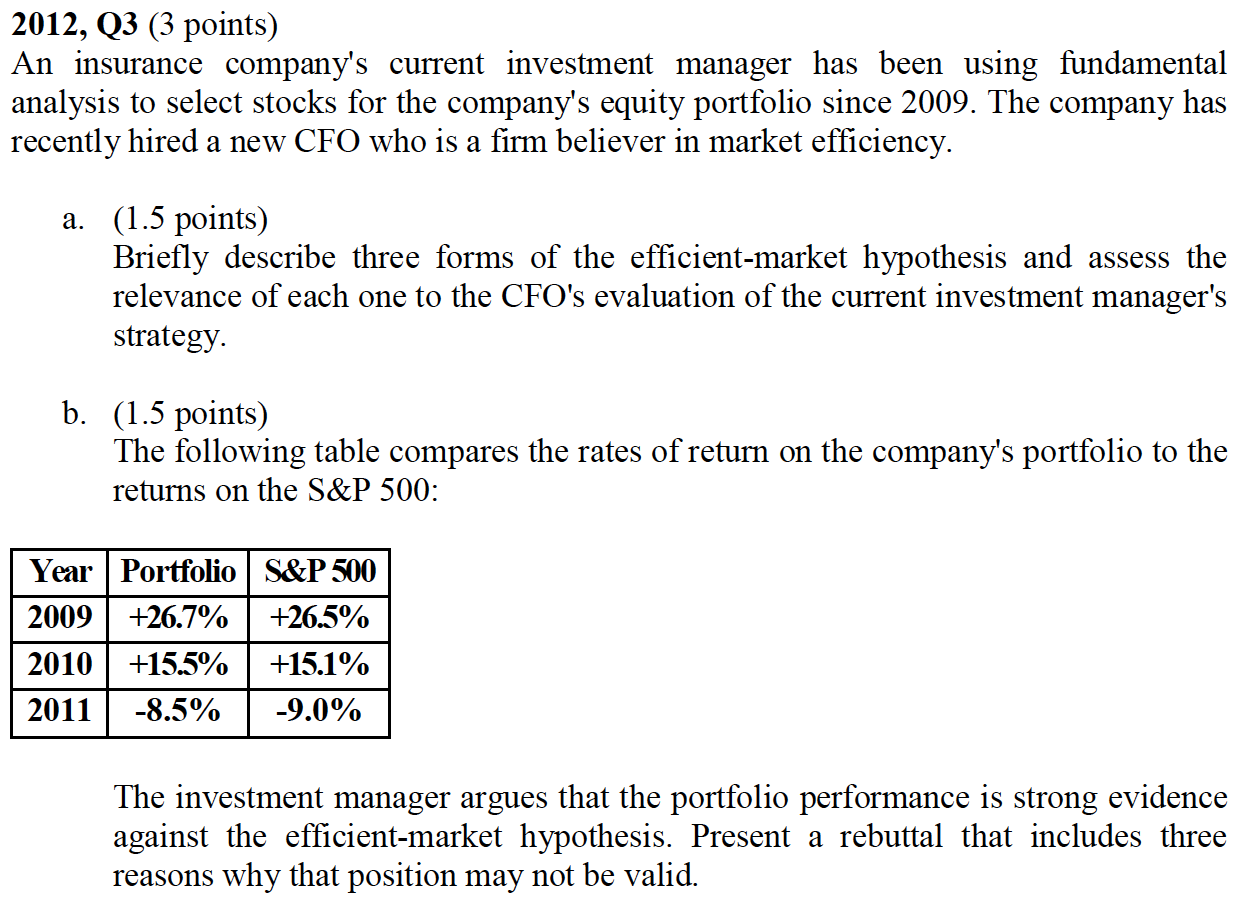
\includegraphics{questions/2012-3Q.png}

\begin{enumerate}
\def\labelenumi{\alph{enumi}.}
\item
  \begin{itemize}
  \tightlist
  \item
    Weak form reflect all past market trading data. Technical analysis
    can't generate XS returns
  \item
    Semi strong: price reflect all public information, fundamental
    analysis won't benefit
  \item
    Strong form: all information is reflected. Unlikely this hold so
    fundamental analysis could work with non public information
  \end{itemize}
\item
  \begin{itemize}
  \tightlist
  \item
    Lucky event: 50\% for each of the 3 years is not impossible
  \item
    Wide variance in return and small difference, might just be random
  \item
    Companys might be taking on more risk to achieve higher returns
  \end{itemize}
\end{enumerate}

 2014, Q6 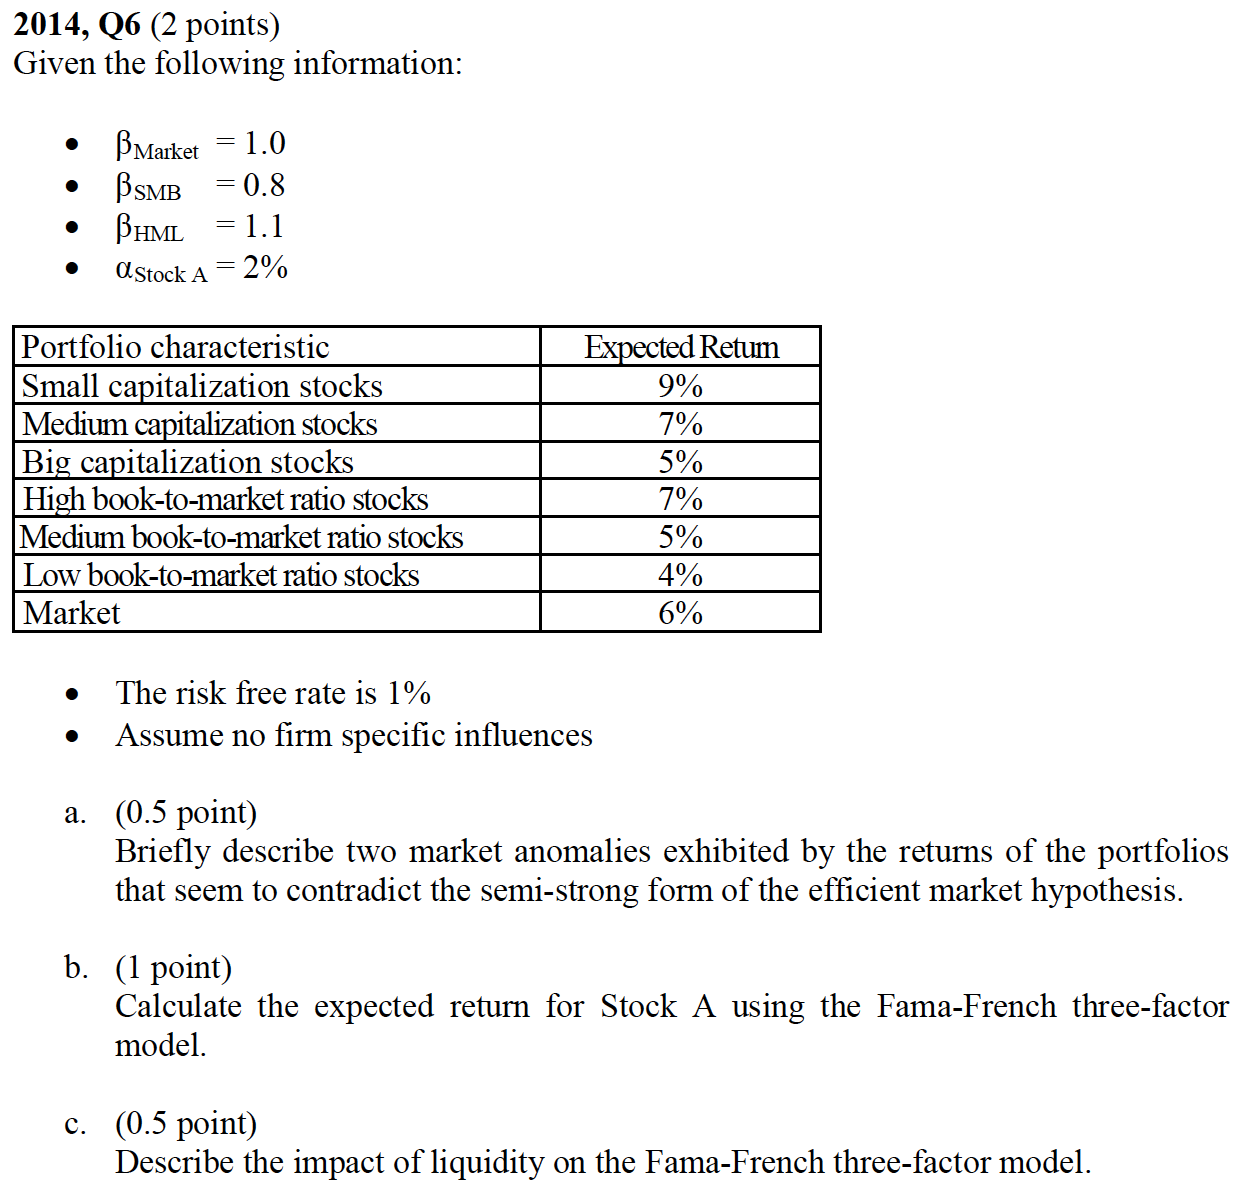
\includegraphics{questions/2014-6Q.png}
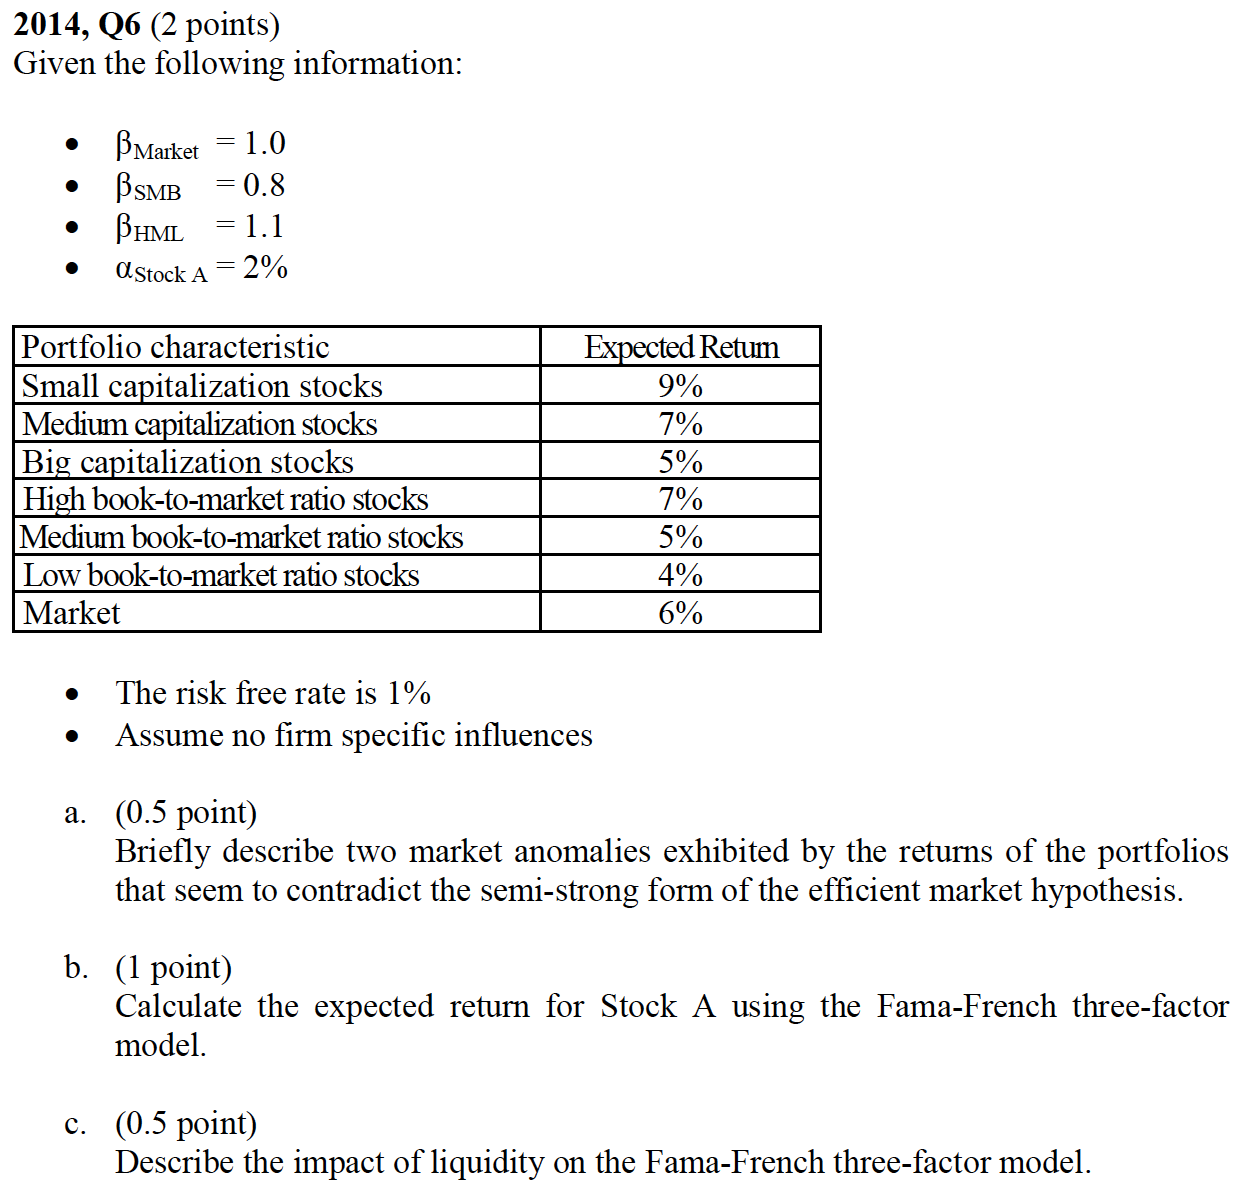
\includegraphics{questions/2014-6Q.png}

\chapter{A7 BKM12: Behavioral
Finance}\label{a7-bkm12-behavioral-finance}

Z. Bodie, A. Kane, A. Marcus

\section{Cliff's Summary}\label{cliffs-summary-6}

Important to know the incorrect
\protect\hyperlink{info-process}{information processing} and
\protect\hyperlink{bias}{behavior bias}

The \protect\hyperlink{limits-to-a}{limits} to arbitrage: mispricing
doesn't disappear, implementation cost and model risk

\begin{itemize}
\tightlist
\item
  Examples on the violation of law of 1 price
\end{itemize}

\protect\hyperlink{bad-behav}{Critique} behavioral finance

How technical anlaysis can work

\begin{itemize}
\tightlist
\item
  Trends indications and market sentiments indicators
\end{itemize}

\subsection{Types of Exam Questions}\label{types-of-exam-questions-6}

\textbf{Concepts}

\begin{itemize}
\tightlist
\item
  2007, Q7: information processing error and market anomaly associated
\item
  2008, Q6: Law of 1 price and violation examples
\item
  2013, Q5: anomaly based on example shown; and associated information
  process error; what efficient market would look like
\end{itemize}

\section{Critique of Financial
Theory}\label{critique-of-financial-theory}

Account for irrationalities in decision making

\begin{itemize}
\item
  \textbf{Incorrect information processing} \(\Rightarrow\) Incorrect
  probability distributions
\item
  Inconsistent/ suboptimal decisions due to \textbf{behavioral biases}
  even if the probability distribution generated was correct
\end{itemize}

\subsection{Information Processing}\label{information-processing}

\textbf{Forecasting Errors}:

\begin{itemize}
\tightlist
\item
  Too much weight assigned to recent experience
\item
  Forecasts are too extreme given the actual level of uncertainty
\end{itemize}

\textbf{Overconfidence}: Overestimate their abilities and think they can
outperform market and trade too much

\begin{itemize}
\tightlist
\item
  Lead to the prevalence of active investment
\end{itemize}

\textbf{Conservatism}: Too slow to update their beliefs in response to
new evidence

\begin{itemize}
\tightlist
\item
  Lead to post earnings announcement drift
\end{itemize}

\textbf{Sample Size Neglect \& Representativeness}: Infer a pattern
based on too small a sample

\begin{itemize}
\tightlist
\item
  Lead to stocks that have best recent performance tend to show
  reversals in a few days due to investor adjusting their initial
  beliefs
\end{itemize}

\subsection{Behavioral Biases}\label{behavioral-biases}

\textbf{Framing}: Decisions are often materially impacted by how the
question is framed

\begin{itemize}
\tightlist
\item
  E.g. preference of discount over surcharge, more risk adverse with
  gain and risk seeking with loss
\end{itemize}

\textbf{Mental Accounting}: Segregate decisions

\begin{itemize}
\tightlist
\item
  E.g. Segment their investment portfolios into pieces which go towards
  different goals and they will have different risk attitudes to each
  piece
\end{itemize}

\textbf{Regret Avoidance}: Unconventional decisions that turned out to
be wrong will have more regret

\textbf{Affect}: Good or bad feeling investors may associate with
investing in a stock

\begin{itemize}
\tightlist
\item
  E.g. Socially responsible firms may generate higher affect
  \(\Rightarrow\) Drive up the prices as investors prefer them
  \(\Rightarrow\) Lower risk adjusted returns
\end{itemize}

\textbf{Prospect Theory}:

Modifies the standard definition of risk averse investors

Utility depends on changes in wealth instead of level of wealth

There is diminishing return of utility as wealth increases but in
addition it shows that investors become risk seeing as they begin to
lose money

\begin{figure}[htbp]
\centering
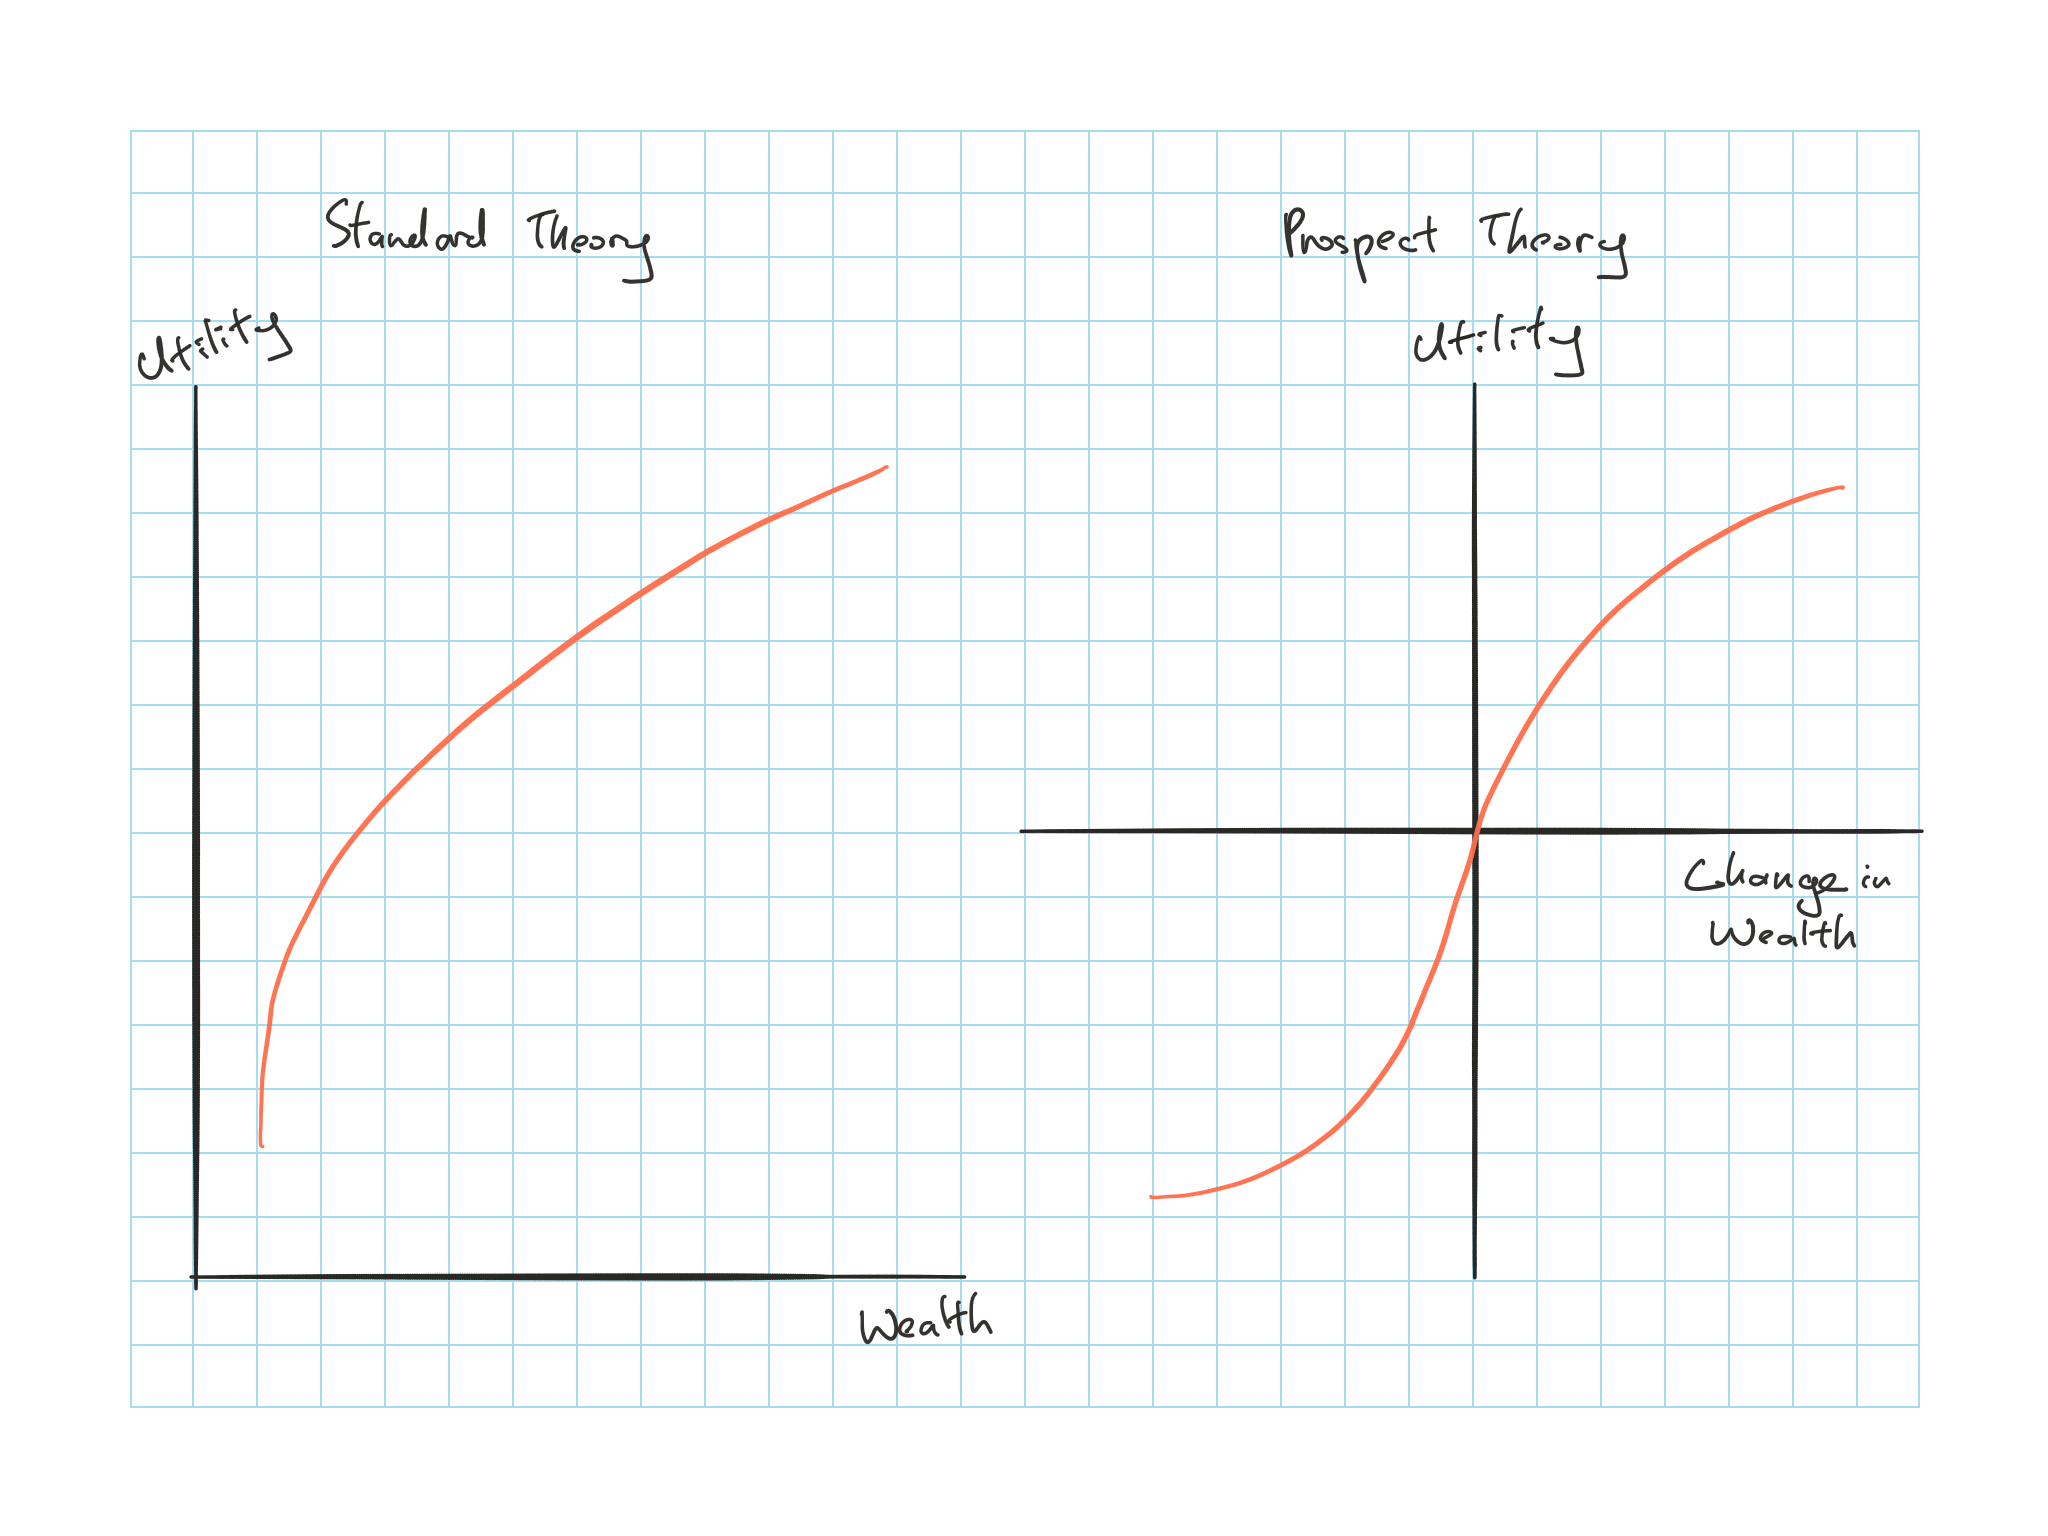
\includegraphics{figures/Exam 9 - 11.png}
\caption{alt text}
\end{figure}

\section{Limits to Arbitrage}\label{limits-to-arbitrage}

Actions for arbitrageurs are limits \(\Rightarrow\) Price
irrationalities can continue

\textbf{Fundamental Risk}: Mispricing are not necessarily going to
disappear, so it's not actually risk free

\textbf{Implementation Costs}: There are limitations to short selling
e.g.~short notice to return the security and some investors are not
permitted to short sell

\textbf{Model Risk}: Fault in the arbitrageur's model that falsely
indicate a mispricing

\section{Violations of the Law of One
Price}\label{violations-of-the-law-of-one-price}

Examples where the law of one price has been violated

\subsection{Siamese Twin Companies}\label{siamese-twin-companies}

When Shell and Royal Dutch Petroleum merged, the profits are set to
split 40/60

\(\hookrightarrow\) Royal Dutch shares should be 150\% of Shells but the
price relativity deviated from the 150\% level for extended period

\begin{itemize}
\tightlist
\item
  Arbitrageurs who tried to profit may have lost money as there were
  periods of time where the deviations actually grew in size
\end{itemize}

\subsection{Equity Carve-outs}\label{equity-carve-outs}

When 3Com spun off Palm, each 3Com shareholder gets 1.5 shares of Palm

3Com shares should be traded for at least 1.5x of Palm but Palm was
traded for more

Arbitrageurs were not able to exploit this by short selling Palm as not
enough shares were available for short selling

\subsection{Closed-End Funds}\label{closed-end-funds}

They typically trade at discount or premium of net asset value

Not a true violation as the fund incurs expenses which will reduce the
share prices

\(\dfrac{\text{Premium}}{\text{Net Asset Value}} = \dfrac{\text{Price} - \text{NAV}}{\text{NAV}} = \dfrac{\alpha - \varepsilon}{\delta + \varepsilon - \alpha}\)

\begin{itemize}
\item
  \(\delta\) = Dividend yield; \(\varepsilon\) = Expense ratio
\item
  Fund will sell at a premium is \(\alpha > \varepsilon\)
\end{itemize}

\section{Critique of Behavioral
Finance}\label{critique-of-behavioral-finance}

\textbf{Unstructured}: Allows virtually any anomaly to be explained by a
combination of irrationalities

\begin{itemize}
\tightlist
\item
  Critics would have more faith in behavioral finance if it provides a
  single behavioral characteristic that explains a range of anomalies
\end{itemize}

\textbf{Inconsistent}: Some anomalies are inconsistent in their support
for one irrationality vs another

\textbf{Benchmark}: Picking the wrong benchmark can produce an apparent
abnormality

\section{Technical Analysis}\label{technical-analysis-1}

Behavioral Finance suggest that technical analysis will be successful in
many cases due to irrationalities in decision making from investors

\textbf{Disposition effect} where investors hold on to losing
investments because they are reluctant to realize losses \(\Rightarrow\)
Slow down the adjustment of the share price to the appropriate value

\textbf{Overconfidence} investors trade more \(\Rightarrow\)
Relationships between trading volume and market returns

\begin{itemize}
\tightlist
\item
  Technical analyst uses volume data to capture this
\end{itemize}

\textbf{Irrational factors} can disturb market fundamentals and
technical analysis can exploit the corrections

\subsection{Trends \& Corrections}\label{trends-corrections}

Technical analysis has to do with uncovering trends

\textbf{Moving Averages}

Average stock price over an interval

\begin{itemize}
\item
  Falling stocks' moving average \textgreater{} current price
\item
  If market breaks through the moving average line from below = bullish
  signal as it's a sign of a shift from falling trend to rising trend
\item
  \textbf{Elliott wave theory} Decomposes the actual movements into long
  term and short term wave cycles, buy when the long term direction is
  positive
\end{itemize}

\textbf{Relative Strength}

Measures how the stock has performed relative to the industry or market

\begin{itemize}
\tightlist
\item
  Ratio of the stock price vs market index
\end{itemize}

\textbf{Breadth}

Measures how widely the movement in the market index is reflected in the
price movements of all stocks

\begin{itemize}
\tightlist
\item
  e.g.~measure the spread between the \# of stocks that advance and
  decline, as \# of advances \textgreater{} \# of declines by a wider
  margin the market is viewed as being stronger
\end{itemize}

\subsection{Sentiment Indicators}\label{sentiment-indicators}

Methods to measure market sentiment

\textbf{Trin Statistics}

Market advances are considered to be stronger when they are accompanied
by stronger trading volumes

\(\text{Trin} = \dfrac{\text{Vol. Declining}/\text{# Declining}}{\text{Vol. Advancing}/\text{# Advancing}}\)

\begin{itemize}
\tightlist
\item
  Ratio \textgreater{} 1.0 are bearish
\end{itemize}

\textbf{Confidence Index}

Based on bond market data assuming actions of bond traders reveal trends
that will later follow in the stock market

\(\text{Confidence Index} = \dfrac{\text{Avg yield on top 10 rated corporate bonds}}{\text{Avg yield on intermediate 10 rated corporate bonds}}\)

\begin{itemize}
\tightlist
\item
  Approaches 100\% when traders are optimistic as they'll require
  smaller default premiums
\end{itemize}

\textbf{Put/ Call Ratio}

\(\dfrac{\text{o/s put options}}{\text{o/s call options}}\)

\begin{itemize}
\tightlist
\item
  Increase in the ratio is a bearish sign as put options profit from
  falling markets
\end{itemize}

\section{Past Exam Questions}\label{past-exam-questions-6}

n/a

\chapter{A8 BKM13: Empirical Evidence on Security
Returns}\label{a8-bkm13-empirical-evidence-on-security-returns}

Z. Bodie, A. Kane, A. Marcus

\section{Cliff's Summary}\label{cliffs-summary-7}

\textbf{Base CAPM Test}

Know the idea of the 2 pass regression and the
\protect\hyperlink{2-pass-caveat}{caveat}

Market index not efficient

\begin{itemize}
\tightlist
\item
  Only the MV efficient hypotheis is testable
\item
  CAPM not testable unless we know the composition of the true market

  \begin{itemize}
  \tightlist
  \item
    Benchmarkt error as well
  \end{itemize}
\item
  Inefficient proxy
\end{itemize}

Measure error for \(\beta\)

\begin{itemize}
\tightlist
\item
  Measurement error of \(\beta\) will drive the slop down and intercept
  up
\item
  Test not high power enough to detect
\item
  Use portfolio to reduce measurement error of \(\beta\)
\end{itemize}

\textbf{Multifactor CAPM and APT Test}

Labor income test

\begin{itemize}
\item
  Add log market equity (for firm size), labor income (for human
  capital), value weighte index, premium on low and high grade bond (for
  state of economy)
\item
  Rejected CAPM
\end{itemize}

Macro factor model

\begin{itemize}
\tightlist
\item
  2 pass regression with bunch of variables, but only 3 shows predictive
  power
\end{itemize}

Fama French

\begin{itemize}
\tightlist
\item
  2 pass regression again and shown to be better than CAPM
\end{itemize}

Risk based interpretation

\begin{itemize}
\tightlist
\item
  HML and SMB captures business cycle risk
\item
  Has time varying \(\beta\)
\item
  \(\beta\) is shown to be counter cyclical with economies
\item
  Value factor may indeed be proxy for risk not capture in CAPM
  \(\beta\)
\end{itemize}

Behavioral

\begin{itemize}
\tightlist
\item
  Market irrationality
\item
  Glamour firm under perform
\end{itemize}

Momentum

\textbf{Liquidity}

Characeristics of liquidity

Measure with price reversals after large trade or asymmetric information

Get liquidity \(\beta\) and see if higher liquidity \(\beta\) goes with
higher price

\textbf{Equity Premium Puzzle}

XS return too high based on reasonable level of risk aversion

Various potential explanation

\begin{itemize}
\tightlist
\item
  Consumption growth
\item
  Unexpected higher return
\item
  Survivorship bias
\item
  Extent CAPM to account for income shock and investor life cycle
\item
  Behavioral like narrow framing and loss aversion
\end{itemize}

\subsection{Types of Exam Questions}\label{types-of-exam-questions-7}

\textbf{CAPM Test}

\begin{itemize}
\tightlist
\item
  2000, Q12: coefficient of 2 pass regression and caveat to the test

  \begin{itemize}
  \tightlist
  \item
    Volatile return; Not true market portfolio; sampling error of
    \(\beta\); Can not borrow at risk free
  \end{itemize}
\item
  2001, Q11: Improvement of CAPM to include state of economy (low and
  high bonds) and market value of equity (size)
\end{itemize}

\section{Tests of CAPM}\label{tests-of-capm}

Tests of various component of CAPM

\subsection{Expected Return and Beta}\label{expected-return-and-beta}

Early test of CAPM
\(\operatorname{E}[r_i] = r_f + \beta_i \left( \operatorname{E}[r_M] - r_f \right)\)

\textbf{1) Sample data}

Select a sample period (e.g.~60mos) and for each incremental period
(month) \(t\) collect:

\begin{itemize}
\tightlist
\item
  \(r_{it}\): rates of return of \(n\) stocks
\item
  \(r_{Mt}\): market proxy (return?)
\item
  \(r_{ft}\): risk free rate for the incremental period \(t\) (1 month)
\end{itemize}

\textbf{2) Estimate SCL (Security Characteristic Line)}

\(r_{it} - r_{ft} = \alpha_i + b_i(r_{Mt} - r_{ft}) + e_{it}\)

Estimate \(\beta\) via first-pass regression for each of the 100 stocks

Recall SCL from BKM8 (\(\operatorname{E}[r]\) vs \(\sigma\))

\textbf{3) Estimate SML (Security Market Line)}

Estimate the \(\gamma\)'s via the second-pass regression using the \(n\)
\(\beta\)s from the different companies in step 2

\(\overline{r_i - r_f} = \gamma_0 + \gamma_1 \beta_i + \gamma_2 \sigma^2(e_i)\)

\begin{itemize}
\item
  \(\overline{r_i - r_f}\) is the sample average over the periods for
  each stock
\item
  \(\sigma^2(e_i)\) is variance of the residual from the first pass
  (variance on the 60 months of residual)
\end{itemize}

Recall SML from BKM9 (\(\operatorname{E}[r]\) vs \(\beta\))

\textbf{Expected Results} if CAPM is valid

\begin{itemize}
\item
  \(\gamma_0 = 0\)
\item
  \(\gamma_1 = \overline{r_M - r_f}\)
\item
  \(\gamma_2 = 0\)
\end{itemize}

\textbf{Test Results}

\begin{itemize}
\item
  Neither \(\gamma_0\) and \(\gamma_2\) are 0
\item
  \(\gamma_1\) is significantly less than the sample average
  \(\overline{r_M - r_f}\)
\end{itemize}

 \textbf{Caveat}

Several difficulties of this testing approach that might have caused the
inconsistent results

\begin{itemize}
\tightlist
\item
  Stock results are volatile, reducing the accuracy of the tests that
  rely on return
\item
  Concerns about the validity of the tests:

  \begin{itemize}
  \tightlist
  \item
    Market index used is not the true market portfolio
  \item
    Large sample error of the \(\beta\) estimates in the first-pass
    regression
  \item
    Investors can't borrow at risk free
  \end{itemize}
\end{itemize}

\subsection{The Market Index}\label{the-market-index}

\textbf{Roll's Critique}

The only testable hypothesis of CAPM is that \emph{the market portfolio
is mean-variance efficient}

\begin{itemize}
\item
  The other implications are based on the market portfolio's efficiency
  and are not independently testable

  \begin{itemize}
  \tightlist
  \item
    e.g.~Linear relationship between \(\operatorname{E}[r]\) and
    \(\beta\)
  \end{itemize}
\end{itemize}

A given sample of observed individual returns can form an infinite
number of ex post portfolios that are mean-variance efficient
\(\Rightarrow\) The \(\beta\)s of these portfolio will satisfy the SML
relation exactly regardless of whether the true market portfolio is
mean-variance efficient

CAPM is not testable unless we know the composition of the true market
and use it in the test \(\Rightarrow\) All assets are required to be
included in the sample

2 difficulties with using proxy such as S\&P 500

\begin{enumerate}
\def\labelenumi{\arabic{enumi})}
\item
  Proxy may be mean-variance efficient even though the true market is
  not
\item
  Most proxies are highly correlated with themselves and the true market

  \begin{itemize}
  \item
    Even if the S\&P is highly correlated, using a different coreelated
    proxy may result in different conclusion
  \item
    Benchmark error: use of incorrect benchmarks in the tests of the
    theory
  \end{itemize}
\end{enumerate}

\textbf{Roll \& Ross Critique}

Tests that reject a positive relationship between the average return \&
\(\beta\) is due to inefficiency in the proxy

\textbf{Kandel \& Stambaugh}

Zero-beta CAPM requires portfolio on the efficient frontier

Need market proxy since we can not easily identify such a portfolio

Market proxy was used to estimate a second pass regression for the
zero-beta CAPM:

\(r_i - r_z = \gamma_0 + \gamma_1 \times \hat{\beta}_i\)

Kandel \& Stambaugh showed that the values of \(\gamma_0\) and
\(\gamma_1\) would be biased by an amount \(\propto\) the efficiency of
the proxy

\(\hookrightarrow\) For the test to be valid, we need an efficient proxy
but it is difficult to test how efficient the proxy is

Given the difficulty in testing CAPM directly, easier to test APT
instead, which produces the same SML given that the portfolio is well
diversified

\subsection{Measurement Error in Beta}\label{measurement-error-in-beta}

If the right handside variable of a regression equation is measured with
error \(\Rightarrow\) slope coefficient will be biased \(\downarrow\)
and the intercept biased \(\uparrow\)

\(\hookrightarrow\) \(\beta\) is measured with error in the second-pass
regression \(\Rightarrow\) Estimated \(\gamma_0\) was \(> 0\) and
\(\gamma_1 < \overline{r_M - r_f}\)

\begin{center}\rule{0.5\linewidth}{\linethickness}\end{center}

Mill \& Scholes used simulated rates of return than followed CAPM in the
first-pass regression to estimate \(\beta\) but the results were
identical to the results based on actual stock returns

\begin{itemize}
\tightlist
\item
  Test was not high power enough
\end{itemize}

\begin{center}\rule{0.5\linewidth}{\linethickness}\end{center}

Modified test to reduce measurement error by using portfolios (instead
of individual securities) to diversify away firm risk \(\Rightarrow\)
More accurate \(\beta\)

\begin{itemize}
\tightlist
\item
  Caveat: Combining reduced the number of observations for the
  second-pass regression
\end{itemize}

\(\hookrightarrow\) Portfolios were constructed to produce the largest
possible dispersion of \(\beta\) coefficients, as this results in more
accurate regression estimates

Fama \& MacBeth tested with the portfolios with the SML below:

\(r_i = \gamma_0 + \gamma_1 \beta_i + \gamma_2 \beta_i^2 + \gamma_3 \sigma(e_i)\)

\begin{itemize}
\item
  \(\gamma_2\) should be 0 based on CAPM but represents the potential
  nonlinearity
\item
  \(\gamma_3\) fluctuated a lot but was not significant
\end{itemize}

\(\hookrightarrow\) Test did not reject CAPM but alternate datasets did
reject the model

\section{Tests of Multifactor CAPM \&
APT}\label{tests-of-multifactor-capm-apt}

Potential supplemental factor to the market risk is a multifactor SML

\begin{itemize}
\tightlist
\item
  Factors that hedge consumption against uncertainty of prices of
  important consumption categories or general inflation (CCAPM)
\item
  Factors that hedge future investment opportunities ( ICAPM
  e.g.~interest rates or market risk premium)
\item
  Factors that hedge assets missing from the market index (non-traded
  asset e.g.~labor income or private business)
\end{itemize}

\subsection{Labor Income}\label{labor-income}

True market portfolio includes aggregate labor income that is (+)-ly
correlated with the market index and have significant value compared to
the value of securities in the index

Stocks that have (+) \(\beta\) on the value of labor will have lower
prices as investor will try to hedge the risk of their human capital by
avoiding those stocks

\begin{itemize}
\tightlist
\item
  Risk premium will be larger than indicated by the standard CAPM
\end{itemize}

To capture human capital:

\begin{enumerate}
\def\labelenumi{\arabic{enumi})}
\item
  Assume \(\Delta\) aggregate labor income \(\approx\) \(\Delta\) value
  of human capital
\item
  Difference between yields on low and high grade bonds \(\approx\)
  state of the economy

  \begin{itemize}
  \tightlist
  \item
    As business cycles may affect the asset \(\beta\) (\(\beta\) are
    conitional on the state of the economy)
  \end{itemize}
\item
  Incorporate firm size adjustment

  \begin{itemize}
  \tightlist
  \item
    \(ME\), market value of equity
  \end{itemize}
\end{enumerate}

\(\hookrightarrow\)
\(\operatorname{E}[R_i] = c_0 + c_{size} \operatorname{log}(ME) + c_{vw}\beta^{vw} + c_{prem}\beta^{prem} + c_{labor}\beta^{labor}\)

\begin{itemize}
\tightlist
\item
  \(\beta^{vw}\) is the \(\beta\) of a value weighted index
\end{itemize}

Test rejected CAPM

\subsection{Macro Factor Model}\label{macro-factor-model}

Variables that may be proxies fro systematic risk factors:

\begin{itemize}
\item
  \(IP\): Growth rate of industrial production
\item
  \(EI\): \(\Delta\) in expected inflation (based on \(\Delta\) in short
  term interest rates)
\item
  \(UI\): Unexpected inflation
\item
  \(CG\): Unexpected \(\Delta\) in risk premium (difference between
  returns of corporate Baa bonds \& long term government bonds)
\item
  \(GB\): Unexpected \(\Delta\) in the term premium (difference between
  returns of long term and short term government bonds)
\end{itemize}

\textbf{First-Pass Regression}

Groups stocks into 20 portfolio based on size

\begin{itemize}
\tightlist
\item
  Size is expected to be associated with average stock returns
\end{itemize}

Based on 5 years of data, regression on each of the group

\(r = a + \beta_M r_M + \beta_{IP} IP + \beta_{EI} EI + \beta_{UI} UI +\beta_{CG} CG + \beta_{GB} GB + e\)

\textbf{Second-Pass Regression}

\(\beta\)s from first-pass regression were used for the second-pass
regression on the 20 portfolios

\(r = \gamma_0 + \gamma_M \beta_M + \gamma_{IP} \beta_{IP} + \gamma_{EI} \beta_{EI} + \gamma_{UI} \beta_{UI} +\gamma_{CG} \beta_{CG} + \gamma_{GB} \beta_{GB} + e\)

\begin{center}\rule{0.5\linewidth}{\linethickness}\end{center}

Regression was ran twice using value weighted NYSE and equally weighted
NYSE

Neither market index is statistically significant (\(|t|\) \textless{}
2)

\(IP\), \(CG\), and \(UI\) showed significant explanatory power

\subsection{Fama French 3 Factor
Model}\label{fama-french-3-factor-model}

Divide stocks into 6 portfolio based on B:M ratios (Low Mid High) and
size (Small Big)

\(\operatorname{E}[r_i] - r_f = \alpha_i + b_i [\operatorname{E}[r_M] - r_f] + s_i \operatorname{E}[SMB]+ h_i \operatorname{E}[HML]\)

First-pass regression: to estimate factors \(b_i\) \(s_i\) and \(h_i\),
intercept should be 0

Comparison of actual returns of US stocks to returns by CAPM and FF
showed that FF does a better job of predicting the returns

\subsection{Risk Based
interpretations}\label{risk-based-interpretations}

Liew \& Vassalou:\\
Returns on style portfolio (HML or SMB) did seem to predict GDP growth
\(\Rightarrow\) Factors capture components of business cycle risk

\begin{itemize}
\tightlist
\item
  Based on comparing return in the years before good GDP growth - return
  before poor growth
\end{itemize}

\begin{center}\rule{0.5\linewidth}{\linethickness}\end{center}

Petkova \& Zhang:\\
Similar test above using conditional CAPM (\(\beta\) and risk premium
vary and co-vary over time)

Relationship between \(\beta\) and \(R_M\)

\begin{itemize}
\item
  Value firms typically have larger amounts of tangible capital
  \(\Rightarrow\) More exposed to the risk of economic downturn due to
  investment irreversibility as they will suffer from XS capacity
  \(\Rightarrow\) Higher \(\beta\) during down markets
\item
  Evidence also show market risk premium \(R_M\) is higher during down
  markets
\end{itemize}

\(\hookrightarrow\) (+) correlation between \(\beta\) and \(R_M\) for
higher B:M value firms

\begin{center}\rule{0.5\linewidth}{\linethickness}\end{center}

Try to prove the above by fitting \(\beta\) and \(R_M\) to state
variables that summarize the state of the economy

\begin{itemize}
\tightlist
\item
  \(DIV\): Market dividend yield
\item
  \(DEFLT\): Default spread on corporate bonds
\item
  \(TERM\): Term structure spread
\item
  \(TB\): 1 month t bill rate
\end{itemize}

\(\begin{array}{cccc}  R_{HML} &= \alpha + &\beta &R_{Mt} + e \\  &= \alpha + &\underbrace{[b_0 + b_1 DIV_t + b_2 DEFLT_t + b_3 TERM_t + b_4 TB_t]}_{\text{time varying }\beta} &R_{Mt} + e_i \\ \end{array}\)

Equation to tie the market risk premium to the state variables

\(r_{Mt,t} - r_{ft} = c_0 + c_1 DIV_t + c_2 DEFLT_t + c_3 TERM_t + c_4 TB_t + e_t\)

Results showed that \(\beta\) is counter cyclical, negative in good
economies and positive during down markets

Test indicated that the value factor may indeed be a proxy for risks not
fully captured by the standard CAPM \(\beta\)

\subsection{Behavioral Explanations}\label{behavioral-explanations}

Value premium arises due to market irrationality

\begin{itemize}
\tightlist
\item
  Analysts extrapolate the performance too far into the future
  \(\Rightarrow\) Overestimate the value of firms with recent good
  performance \(\Rightarrow\) Prices fall when market realizes its
  mistakes
\end{itemize}

\(\hookrightarrow\) Glamour firms will often under perform value firms

\begin{itemize}
\tightlist
\item
  Glamor firms = those with recent good performance, high prices and
  lower B:M ratios
\end{itemize}

Studies below support the view of market irrationality

\begin{center}\rule{0.5\linewidth}{\linethickness}\end{center}

Overreaction study (Chan, Karceski and Lakonishok)

\begin{itemize}
\item
  Groups firms into deciles based on income growth for the past 10 years
\item
  Measured B:M value at the beginning and end of 5 years period and
  found:

  \begin{itemize}
  \item
    Ending B:M falls steadily with growth \(\Rightarrow\) Past growth
    has therefore been extrapolated and incorporated into the price
  \item
    Beginning B:M has minimal (small positive) relationship with growth
    \(\Rightarrow\) Glamour firms do not outperform other firms in terms
    of future income growth
  \end{itemize}
\end{itemize}

\begin{center}\rule{0.5\linewidth}{\linethickness}\end{center}

Performance of value vs glamour stocks (La Porta, Lakonishok, Shleifer
\& Vishny)

\begin{itemize}
\item
  Focused on the stock price performance of each type once earnings were
  released
\item
  Found that value stocks consistently outperform glamour stocks
\item
  Could be due to market being disappointed by the earnings releases of
  growth stocks because the expectations were too high
\end{itemize}

\subsection{Momentum}\label{momentum}

Momentum has been proposed to be included in the Fama French model as a
4\textsuperscript{th} factor

This may be what was causing the \(\alpha\) in the 3 factor model

However it is difficult to justify/ explain this factor and unclear to
see what type of risk this would be acting as a proxy for

\section{Liquidity and Asset Pricing}\label{liquidity-and-asset-pricing}

Liquidity's impacts on asset's \(\operatorname{E}[r]\)

\begin{enumerate}
\def\labelenumi{\arabic{enumi})}
\tightlist
\item
  Transaction costs (bid/ask spread)
\item
  Liquidity risk (\(\Delta\) in liquidity cost)
\end{enumerate}

Difficult to estimate as they are often unobservable

Characteristics of \textbf{Liquidity}

\begin{itemize}
\tightlist
\item
  Trading costs
\item
  Ease of sale
\item
  Price concessions required to motivate a quick transaction
\item
  Market depth
\item
  Price predictability
\end{itemize}

\(\hookrightarrow\) Difficult to have a single statistic to capture all
the above components

\begin{center}\rule{0.5\linewidth}{\linethickness}\end{center}

Common methods to measure liquidity focus on the price impact:

\textbf{Price reversals follow large trades}:

\begin{itemize}
\item
  Based on the assumption that reversals on the following day would be a
  symptom of price impact of the initial trade
\item
  \(ILLIQ = \text{M-thly Avg of Daily}\left[ \dfrac{\mid Return_{stock}\mid}{\text{Dollar Volume}} \right]\)
\item
  Focus on the relationship between large trades and price movements

  \begin{itemize}
  \item
    Measures the price impact per dollar of transactions
  \item
    Measures both liquidity cost and liquidity risk
  \end{itemize}
\end{itemize}

\textbf{Asymmetric information}:

\begin{itemize}
\item
  Based on the assumption that the price impact is due to asymmetric
  information
\item
  Regressions are used to determine how much of the price impact is due
  to information
\item
  Liquidity risk will be cause by changes in the prevalence of
  informationally motivated trades
\end{itemize}

\begin{center}\rule{0.5\linewidth}{\linethickness}\end{center}

Use one of the above 2 method to derive the level of market wide
illiquidity \(\Rightarrow\) Calculate liquidity beta (sensitivity of
returns to \(\Delta\) liquidity) of an individual stock

If stocks with higher liquidity \(\beta\) have higher returns
\(\Rightarrow\) Liquidity is a priced factor

Pistor \& Stambaugh study:

\begin{itemize}
\item
  Examine whether liquidity risk is a priced factor
\item
  Sorted sample portfolio into deciles, based on the liquidity \(\beta\)
\item
  Calculate the average \(\beta\) of each decile using a model that
  ignores liquidity (standard CAPM and FF 3 factor)
\item
  Found that \(\alpha\) did rise substantially for the higher liquidity
  \(\beta\) deciles \(\Rightarrow\) Supported the view that liquidity
  risk was a priced factor
\end{itemize}

\section{Equity Premium Puzzle}\label{equity-premium-puzzle}

\textbf{Equity premium puzzle}:\\
Historical XS returns on risky assets in the US are too large to be
consistent with economic theory and reasonable levels of risk aversion

\subsection{Consumption Growth \& Market Rates of
Return}\label{consumption-growth-market-rates-of-return}

ICAPM implies that investors make decisions based on their lifetime flow
of consumption and not just their current wealth

To measure consumer well being we should focus on the consumption flow
that wealth can support

\begin{center}\rule{0.5\linewidth}{\linethickness}\end{center}

CAPM \(\beta = \dfrac{\operatorname{Cov}(r_i, r_M)}{\sigma^2_M}\), based
on the covariance of returns with market return \(\Rightarrow\) Only
focused on just wealth

Should rely on covariance of the market with aggregate consumption:

\(\operatorname{E}[r_M] - r_f = A \cdot \operatorname{Cov}(r_M, r_C)\)

\begin{itemize}
\item
  \(A\): Average coefficient of risk aversion
\item
  \(r_C\): Rate of return on a consumption tracking portfolio that has
  been designed to have the highest possible correlation with growth in
  aggregate consumption
\end{itemize}

Based on reasonable values of \(A\), covariance is much too low to
produce the empirical average XS returns \(\Rightarrow\) Given an
appropriate risk aversion factor, XS returns are too high

\begin{center}\rule{0.5\linewidth}{\linethickness}\end{center}

Study to demonstrate that the Fama French factors are associated with
consumption \(\beta\) (Jagannathan \& Wang)

\begin{itemize}
\item
  High B:M stocks generally have higher consumption \(\beta\)s
\item
  Larger firms generally have lower \(\beta\)s
\end{itemize}

\(\hookrightarrow\) Explanatory powers of the FF factors may be due to
consumption risk

\begin{itemize}
\tightlist
\item
  Also proved that CCAPM model explains returns better than the FF model
\end{itemize}

\begin{center}\rule{0.5\linewidth}{\linethickness}\end{center}

Standard CCAPM focuses on an average investor \(\Rightarrow\) Does not
acknowledge the heterogeneous investor with different level of wealth
and consumption habits

Newer models reflect the different types of investors

\begin{itemize}
\tightlist
\item
  e.g.~incorporate the fact that the covariance between market returns
  and consumption \(\uparrow\) when household holds financial securities
\end{itemize}

\(\hookrightarrow\) Reflecting the heterogeneity may mitigate the
observed equity premium puzzle

\subsection{Expected vs Realized
Returns}\label{expected-vs-realized-returns}

Historical returns of the S\&P 500 relative to the \(r_f\)
\(\upuparrows\) since 1950s

Using average realized returns to derive the risk premium may be the
problem causing the puzzle

Calculate \(\operatorname{E}[r]\) using dividend discount model

\(\operatorname{E}[r] = \dfrac{D_1}{P_0} + g\)

\begin{itemize}
\item
  \(D_1\) = end of year dividend
\item
  \(P_0\) = current stock price
\item
  \(g\) = expected dividend growth rate
\end{itemize}

Model produced a smaller risk premium than actual for the period after
1950 \(\Rightarrow\) High XS returns for the period may have been
\textgreater{} than the rate that investors expected to earn

\(\hookrightarrow\) Unanticipated gains may be responsible for the
equity premium puzzle

\subsection{Survivorship Bias}\label{survivorship-bias}

Equity premium puzzle is based on studies of US stock return

May be caused by survivor-ship bias as the US market has experienced
some of the highest returns during the historical period

\subsection{CAPM Extensions}\label{capm-extensions-1}

CAPM extensions may resolve the equity premium puzzle

Can modify the basic CAPM to account for the observed XS returns by
relaxing some of the standard CAPM assumptions

\begin{itemize}
\item
  Consumers face income shocks (loss of job), the risk of which
  increases during economic downturns
\item
  Investors stage in the life cycle has an impact on their situation
  e.g.~borrowing constraints change over time, younger people will
  typically face more borrowing constraints
\end{itemize}

Study showed that afters accounting for these and other factors, we can
explain the higher risk premium observed in the market

\subsection{Behavioral Explanations}\label{behavioral-explanations-1}

Puzzle may arise due to irrational investor behavior

\textbf{Narrow framing}

Investors evaluate each risk that they are exposed to in isolation
\(\Rightarrow\) Ignore the fact that risk from the stock portfolio has a
low correlation with other components of wealth \(\Rightarrow\) Require
a higher risk premium than indicated by the models

\textbf{Loss aversion}

This will also cause investors to require higher premiums

\section{Past Exam Questions}\label{past-exam-questions-7}


\end{document}
